\chapter{Switching Whole Networks}
\label{chap:switching-whole-networks}
\index{network energization}
\index{transformer!inrush current}
\index{switching overvoltage}
\index{voltage ramp}

\section{General}
\label{sec:whole-network-general}

This chapter examines the transients that occur when an entire network (grid zone) is energized. This situation can occur during grid restoration following a blackout\\ 
The following cases are examined in detail:\\
\begin{itemize}
	\item \texttt{Connecting at minimum voltage in phase R},
	\item \texttt{Connecting the grid zone with phase R at maximum voltage},
	\item \texttt{Connecting at minimum voltage and full remanent flux},
	\item \texttt{Connecting with the main transformer set to minimum voltage},
	
	\item \texttt{Connecting a larger grid zone},
	\item \texttt{Connecting under load}.
	\item \texttt{Connecting with skin effect in the grid impedance},
	\item \texttt{Connecting with a weak feed-in},
	\item \texttt{Slowly ramping up the voltage instead of a switching operation}.
\end{itemize}

\section{Circuit Design}
Open the File \texttt{Switching\_on\_networks.asc}.
The example is a \SI{110}{\kilo\volt} network with five substations.
Three substations are loaded, two are unloaded or have loads that are not yet
connected. The network is supplied through a
\SI{220}{\kilo\volt}/\SI{110}{\kilo\volt} transformer rated
\SI{200}{\mega\volt\ampere}.

The main transformer is represented by a linear magnetizing characteristic
using the transformer parameter \texttt{m=1}. Its voltage source initially rises exponentially so that
the transformer reaches steady state before the network switch closes. The network contains three cable sections and two overhead-line sections. The cables have a total sum length of \SI{10}{\kilo\metre} and generate approximately
\SI{15}{\mega\varunit} of capacitive reactive power (see calculation \ref{calc:whole-network-petersen}). A \SI{40}{\mega\varunit} shunt reactor in bus4 overcompensates the \SI{15}{\mega\varunit} capacitive contribution, leaving a net inductive demand of approximately \SI{25}{\mega\varunit}. 
The energized network therefore tends to reduce rather than raise the voltage (under steady state conditions).

The cable phase-to-earth capacitances are compensated by a Petersen coil at
substation 1. A small capacitance asymmetry is required to create a measurable
neutral displacement voltage. In the model, this is introduced with the
parameter \texttt{cuf} in phase A of line 2.


\section{Petersen-Coil Setting}
\label{sec:whole-network-petersen-setting}

The cable capacitance is \SI{400}{\nano\farad\per\kilo\metre} per phase (see line.lib). For a
total cable length of \SI{10}{\kilo\metre}, the phase capacitance is
\SI{4000}{\nano\farad}.

\begin{calculation}{Compensation current for the complete cable network}{whole-network-petersen}
At \SI{50}{\hertz},
\begin{align}
C&=\SI{400}{\nano\farad\per\kilo\metre}\cdot\SI{10}{\kilo\metre}
  =\SI{4000}{\nano\farad},\\
X_C&=\frac{1}{\omega C}
  =\frac{1}{2\pi\cdot\SI{50}{\hertz}\cdot\SI{4000}{\nano\farad}}
  \approx\SI{796}{\ohm},\\
Q_C&=\frac{U_{\mathrm{LL}}^2}{X_C}
  =\frac{(\SI{110}{\kilo\volt})^2}{\SI{796}{\ohm}}
  \approx\SI{15.2}{\mega\varunit}.
\end{align}

For resonant earth-fault compensation,
\begin{align}
X_{L,\mathrm P}&=\frac{X_C}{3}\approx\SI{265}{\ohm},\\
I_{\mathrm P}&=\frac{U_{\mathrm{LL}}/\sqrt{3}}{X_{L,\mathrm P}}
  \approx\boxed{\SI{239.7}{\ampere}}.
\end{align}
\end{calculation}

The Petersen model uses a rounded setting of \SI{250}{\ampere}. An increase of roughly
\SI{5}{\percent} is useful because internal transformer reactance reduces the
neutral voltage and prevents the ideal coil current from being reached during
an earth fault. This effect was discussed in detail in
\cref{chap:earth-faults}.

\section{Calculation of the Network Resonance}
\label{sec:whole-network-resonance}

The inductances specified on the \SI{220}{\kilo\volt} side must be referred to
the \SI{110}{\kilo\volt} side. With a voltage ratio of 2, impedance and
inductance are divided by $2^2=4$ when referred from the
\SI{220}{\kilo\volt} side to the \SI{110}{\kilo\volt} side. 
The source and transformer inductances are $L_{\mathrm{net}}=\SI{0.0077}{\henry}$ and $L_{\mathrm{Tr}}=\SI{0.154}{\henry}$. The transformer value is obtained from
\texttt{xkos/omega} in \texttt{Trafo\_YY0\_220k\_110k\_200MVA\_Daten.asc}. Thus, ..



\begin{calculation}{Dominant cable-network resonance}{whole-network-resonance}
	\begin{align}
		L_{\mathrm{eq}}&=\frac{L_{\mathrm{net}}}{4}
		+\frac{L_{\mathrm{Tr}}}{4}
		=\frac{\SI{0.0077}{\henry}+\SI{0.154}{\henry}}{4}
		=\SI{0.04}{\henry},\\
		C&=\SI{4000}{\nano\farad},\\
		f_{\mathrm r}&=\frac{1}{2\pi\sqrt{L_{\mathrm{eq}}C}}
		\approx\boxed{\SI{395.8}{\hertz}}.
	\end{align}
\end{calculation}

This result agrees with the approximately \SI{400}{\hertz} peak, which is most clearly visible (after simulation) in
the FFT of the main transformer current in phases B and C in Case 1. Zoom into the interval from 40 ms to 100 ms, then select View → FFT and use the current zoom extent.
Additional harmonics caused by the nonlinear transformer currents are most clearly visible in phase A at 100 Hz, 150 Hz, 200 Hz and 250 Hz.

\section{Rated current of the main transformer}
\label{sec:whole-network-case1-values}

The rated RMS current on the \SI{220}{\kilo\volt} side of the main transformer
is

\begin{equation}
	I_N=\frac{S_N}{\sqrt{3}U_N}
	=\frac{\SI{200}{\mega\volt\ampere}}
	{\sqrt{3}\cdot\SI{220}{\kilo\volt}}
	\approx\boxed{\SI{525}{\ampere}}.
\end{equation}

\noindent For further values of transformer parameters see: \\
Transformer\_110kV\_10KV.asc for the medium voltage transformer and \\
Transformer\_220kV\_110KV.asc for the high voltage transformere


\section{Case 1: Closing at the Phase-R Voltage Zero} 
\label{sec:network-closing-voltage-zero}

NOTE: The ltspice file for all cases except case9 is \texttt{Switching\_on\_networks.asc}.
To view the results in the Waveform Viewer, you must select the appropriate plot file. After the simulation, open the Waveform Viewer window. Select “Plot Settings” / “Open Plot Settings File” and, from the available plots, select one of the corresponding case1 plots. Plots of voltages, currents, and magnetic fluxes are available.
For the different simulations some parameters in the schematic are changed. 
With \texttt{t0=0} the network switch closes at \SI{40}{\milli\second}, when
the phase A voltage crosses zero. The primary phase A current of the main
transformer is then dominated by the magnetizing inrush currents of the
medium-voltage transformers. Closing at voltage zero produces the largest
unidirectional flux offset in Phase A (U). Even without residual flux, the transient flux can
approach twice its steady-state peak starting from zero to about \SI{0.58}{\weber}.

At the same instant, the phase A (U) capacitive charging current is comparatively
small because the applied voltage is close to zero. In phases B (V) and C (W), the
opposite situation occurs: the instantaneous voltages are high, their medium-voltage
transformer flux offsets are smaller, and their initial cable-charging currents
are large. The principal currents decay over approximately
\SI{500}{\milli\second}. The over-voltages depends strongly on the switching instant. 


All three phase currents contain high-frequency components caused by resonances
between the cable capacitances and the source and transformer inductances. An
FFT of a phase A medium-voltage-transformer current also contains many
harmonics (100Hz,150Hz,200Hz,250Hz) of the power frequency because of the nonlinear transformer
magnetizing curves. In phases B and C, a distinct network resonance appears at
approximately \SI{400}{\hertz}.\\

All three medium voltage transformer currents exhibit similar but also slightly different behaviour. Since a Petersen coil is connected to the neutral point of Transformer 1, the inrush-current waveform partly extends below zero. For Transformer 2, a faster decay of the inrush current can be observed. This can be explained by the additional voltage drop caused by the shunt reactor current on Line 2. In Phase A, the shunt reactor carries a current that remains entirely positive (in phase with the transformer). This current causes a greater voltage drop across Line 2 and thus a lower voltage across the transformer. Since the flux of the transformer depends directly on the integral of the voltage, both the flux and the current of the transformer decrease. NOTE: The behaviour described above occurs only if the shunt reactor is turned on simultaneously with the transformer. If the shunt reactor is turned on 10 ms later, its current is out of phase with the transformer current, and the inrush current of the transformer will now decrease more slowly or even rise slightly at first. Try it out by inserting a switch with a switching time of 50 ms before the shunt reactor.

Lines 3 and 4 are overhead lines, so their capacitive charging transients are much lower than those of the cables.
For Schematic and waveforms see figures \ref{fig:figure61}-\ref{fig:figure66}. 
For measured values and signal ranges, see Table \ref{tab:measurement-values-case1}.\\



%\begin{figure}[H]
%	\centering
%	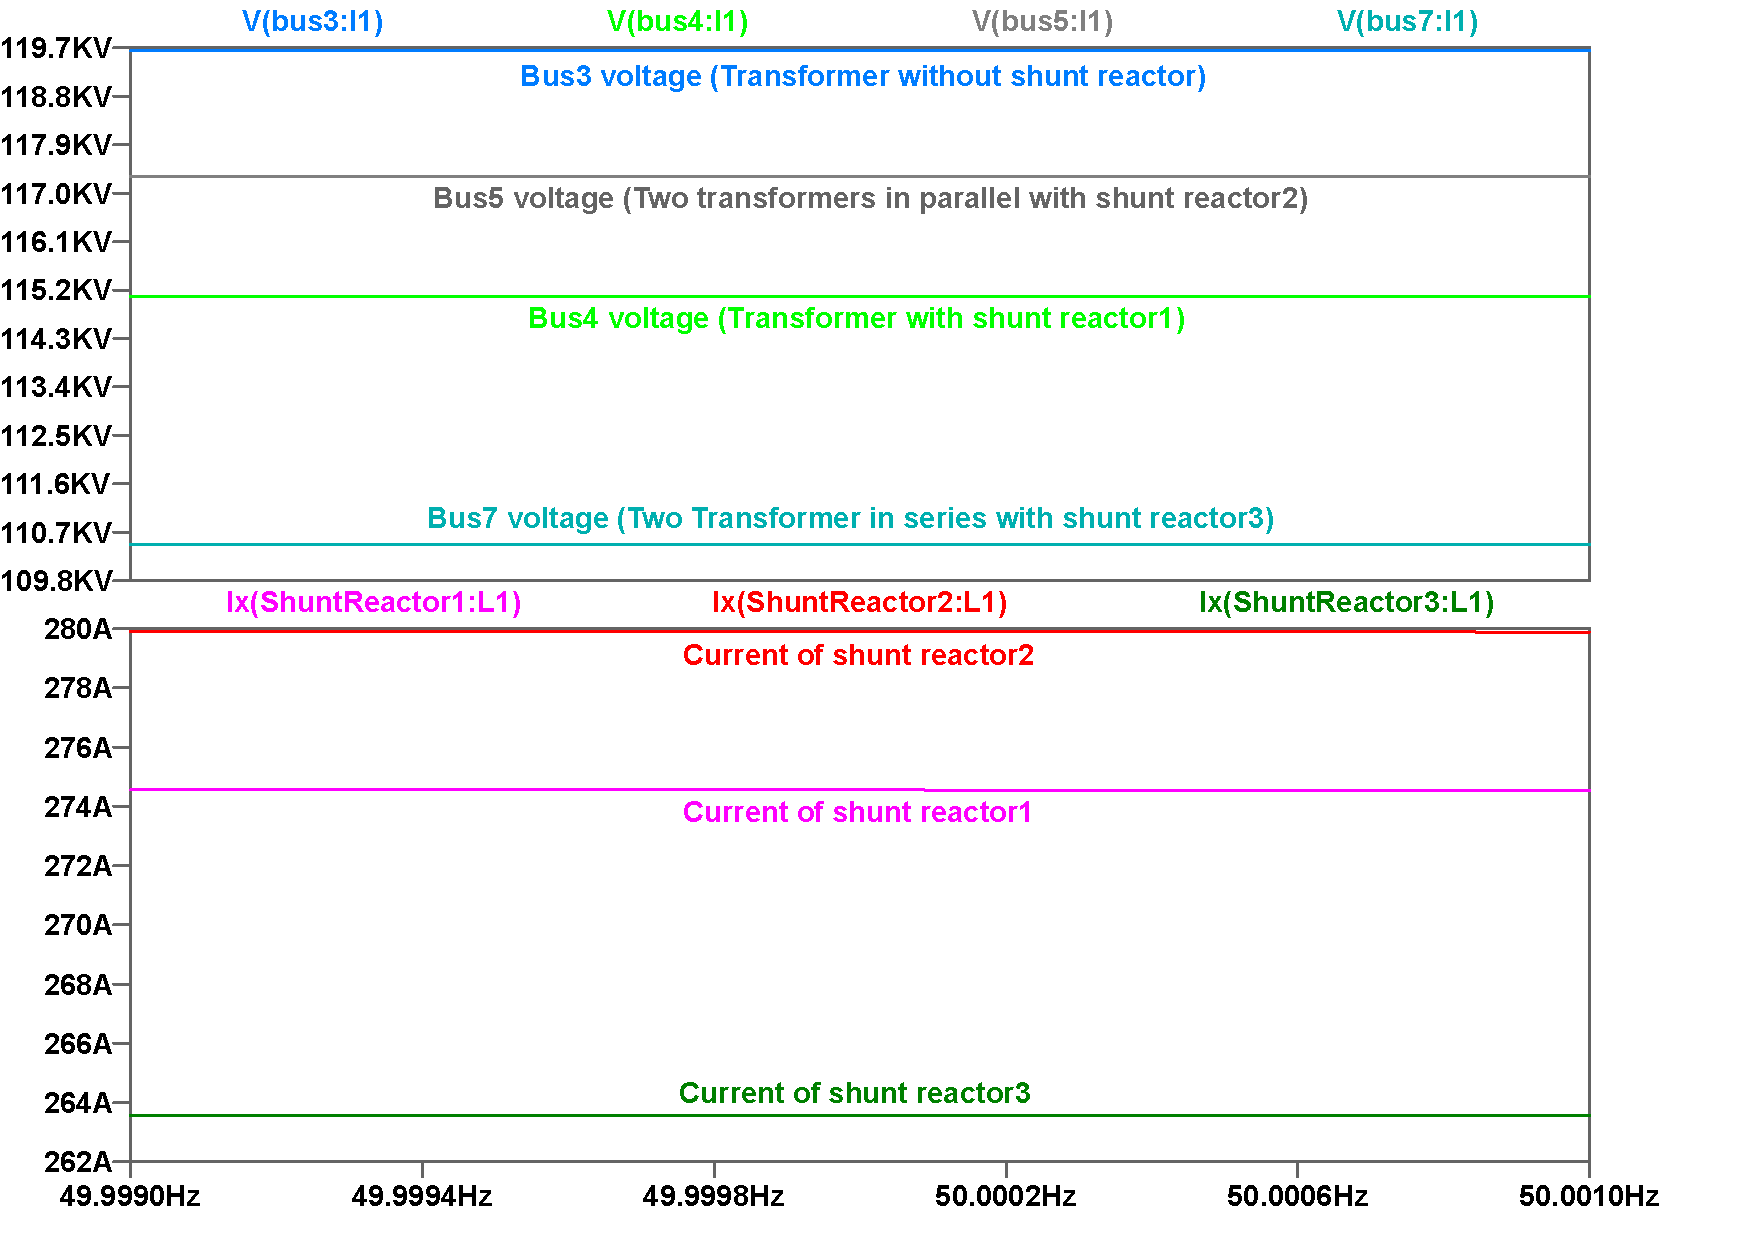
\includegraphics[width=0.90\textwidth]{figures/01_Transformer und shunt reactor/Transformer_and_shunt_reactor_AC_waveform}
%	\caption{AC voltages and currents at the shunt reactors}
%	\label{fig:Transformer_and_shunt_reactor_AC_Waveform}
%\end{figure}

\begin{figure}[H]
	\centering
	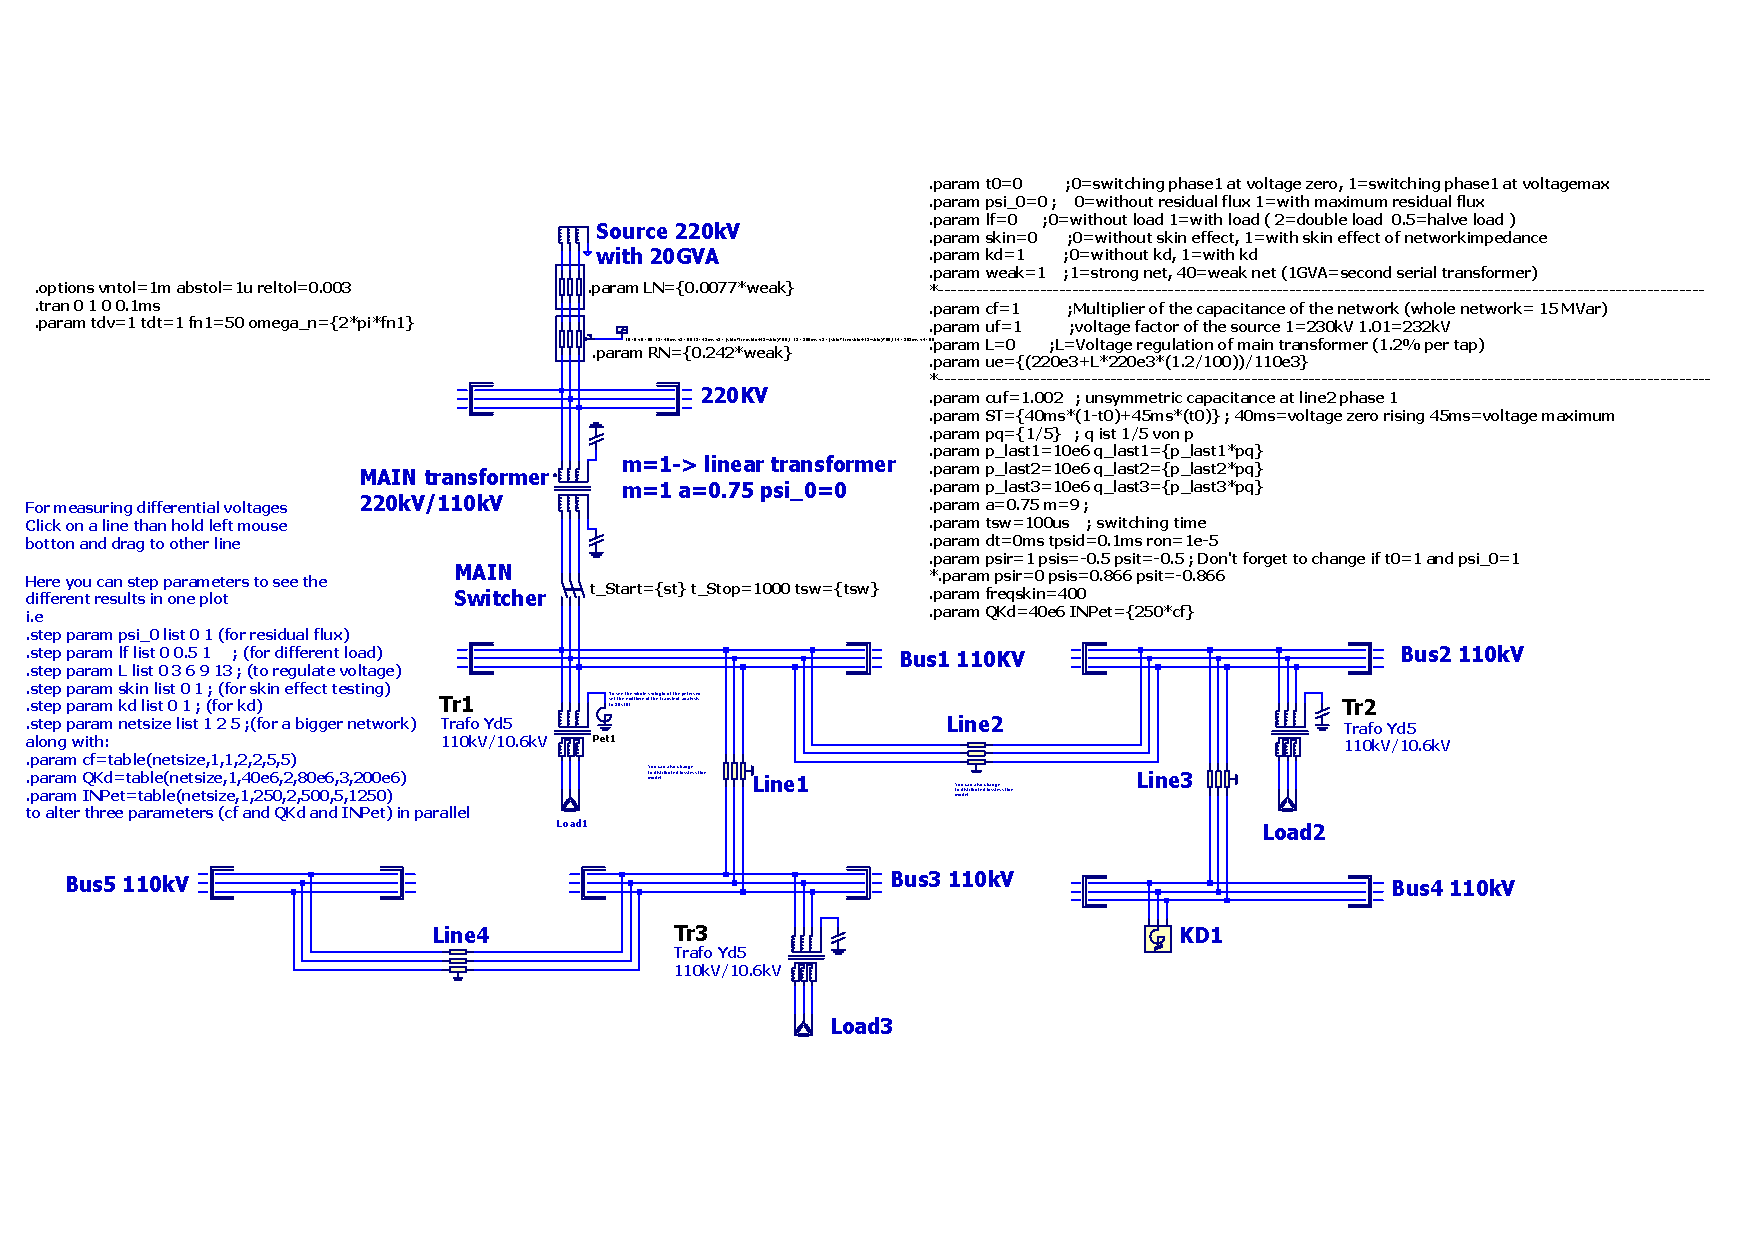
\includegraphics[width=0.9\textwidth]{figures/06_Switching_on_networks/Switching_on_networks_schematic}
	\caption{Switching on networks schematic - case1}
	\label{fig:figure61}
\end{figure}

\begin{figure}[H]
	\centering
	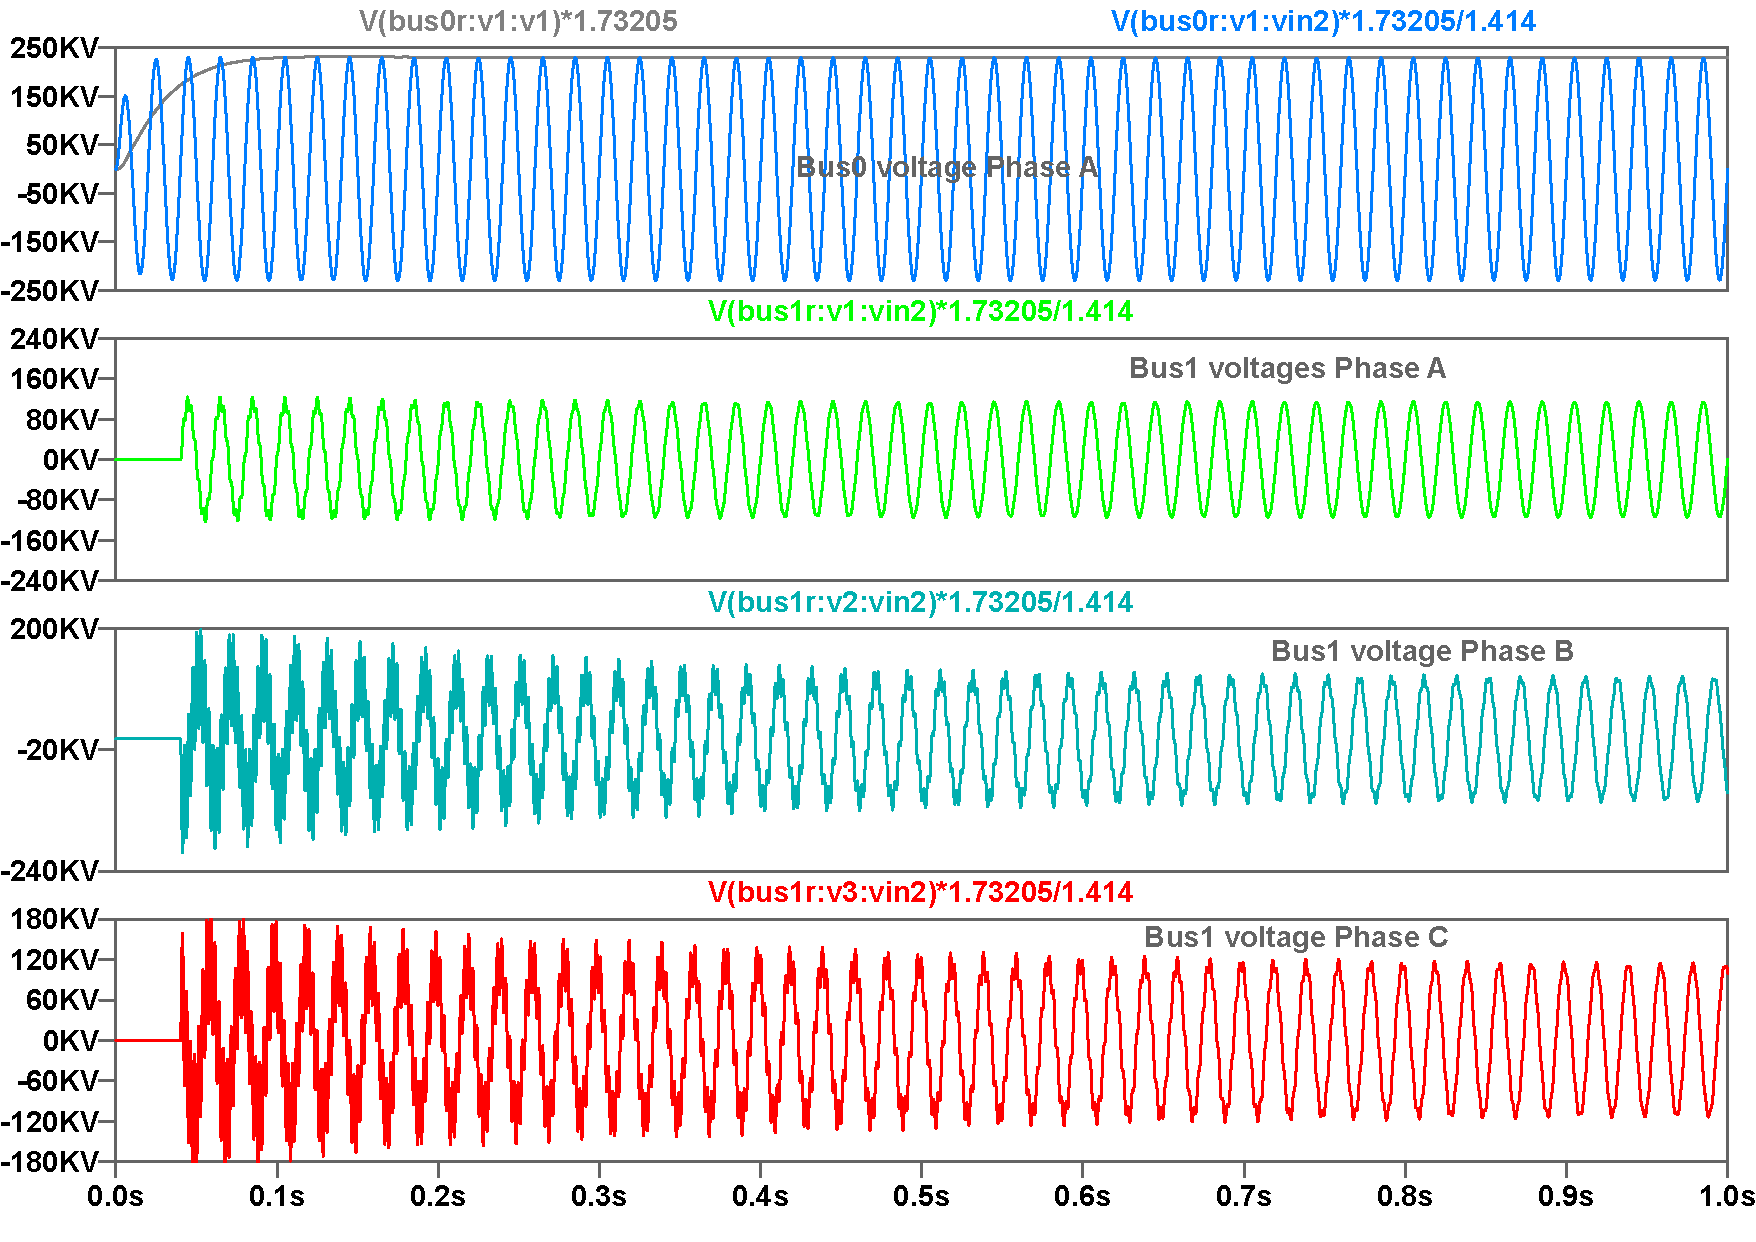
\includegraphics[width=0.90\textwidth]{figures/06_Switching_on_networks/Switching_on_networks_Bus0_Bus1_voltages-case1}
	\caption{Switching on networks voltages - case1}
	\label{fig:figure62}
\end{figure}

\begin{figure}[H]
	\centering
	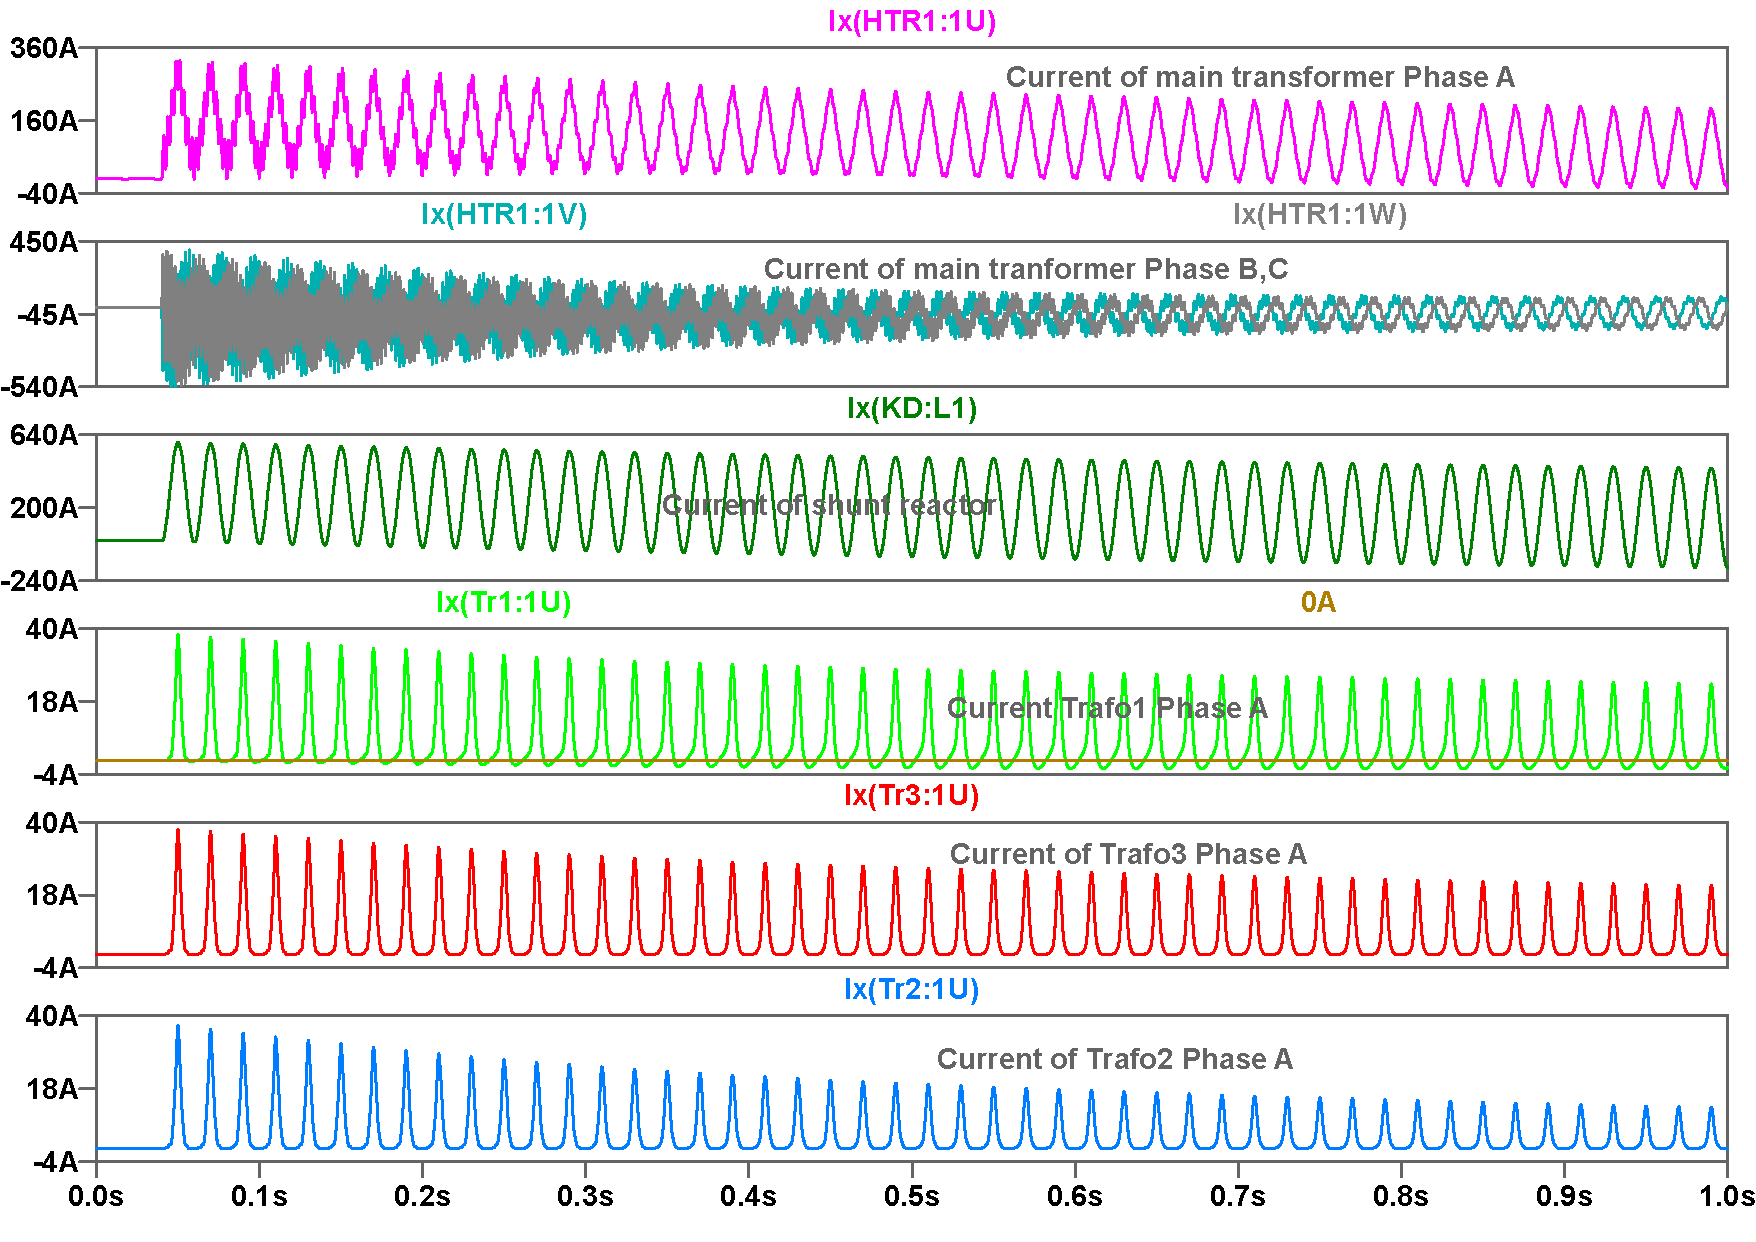
\includegraphics[width=0.90\textwidth]{figures/06_Switching_on_networks/Switching_on_networks_currents-case1}
	\caption{Switching on networks currents - case1}
	\label{fig:figure63}
\end{figure}

\begin{figure}[H]
	\centering
	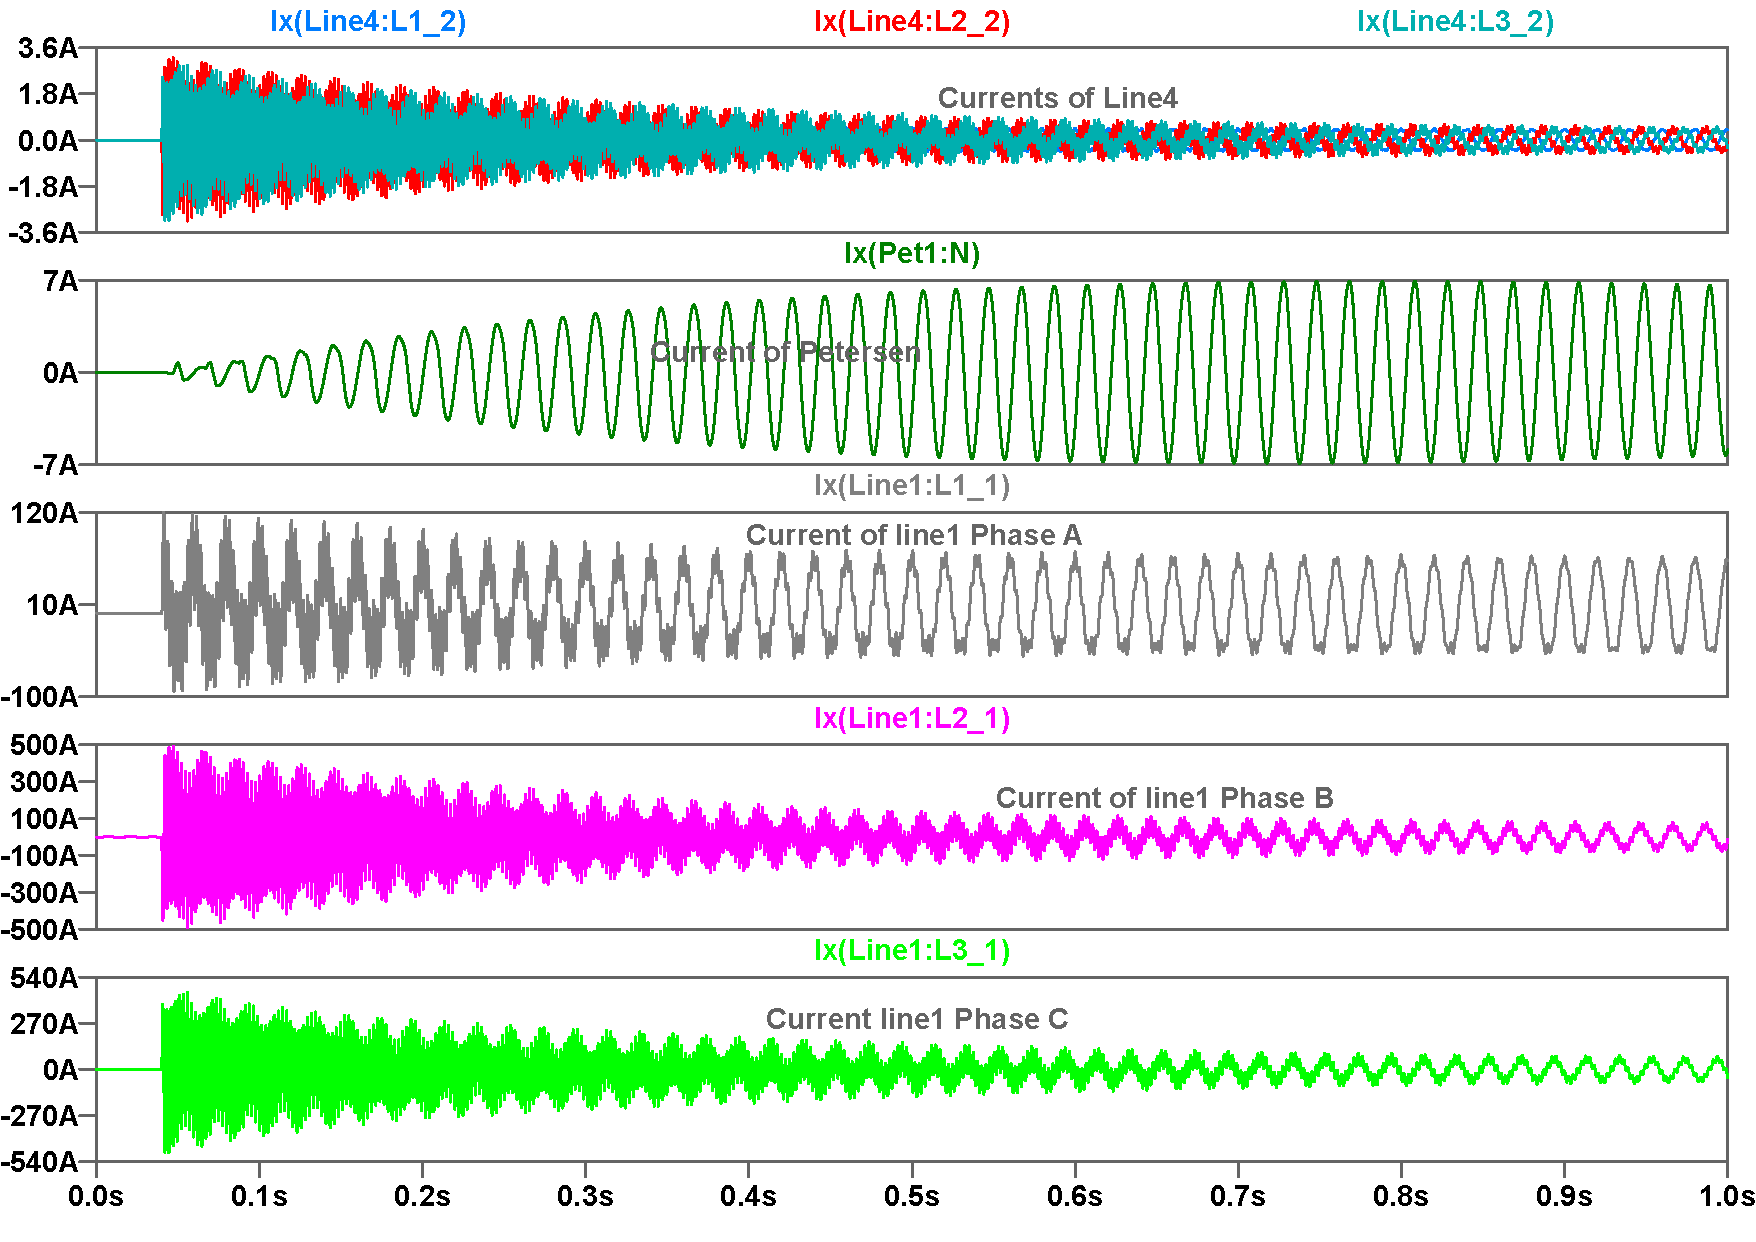
\includegraphics[width=0.90\textwidth]{figures/06_Switching_on_networks/Switching_on_networks_currents_Line1_Line4-case1}
	\caption{Switching on networks currents line1, line4 - case1}
	\label{fig:figure64}
\end{figure}

\begin{figure}[H]
	\centering
	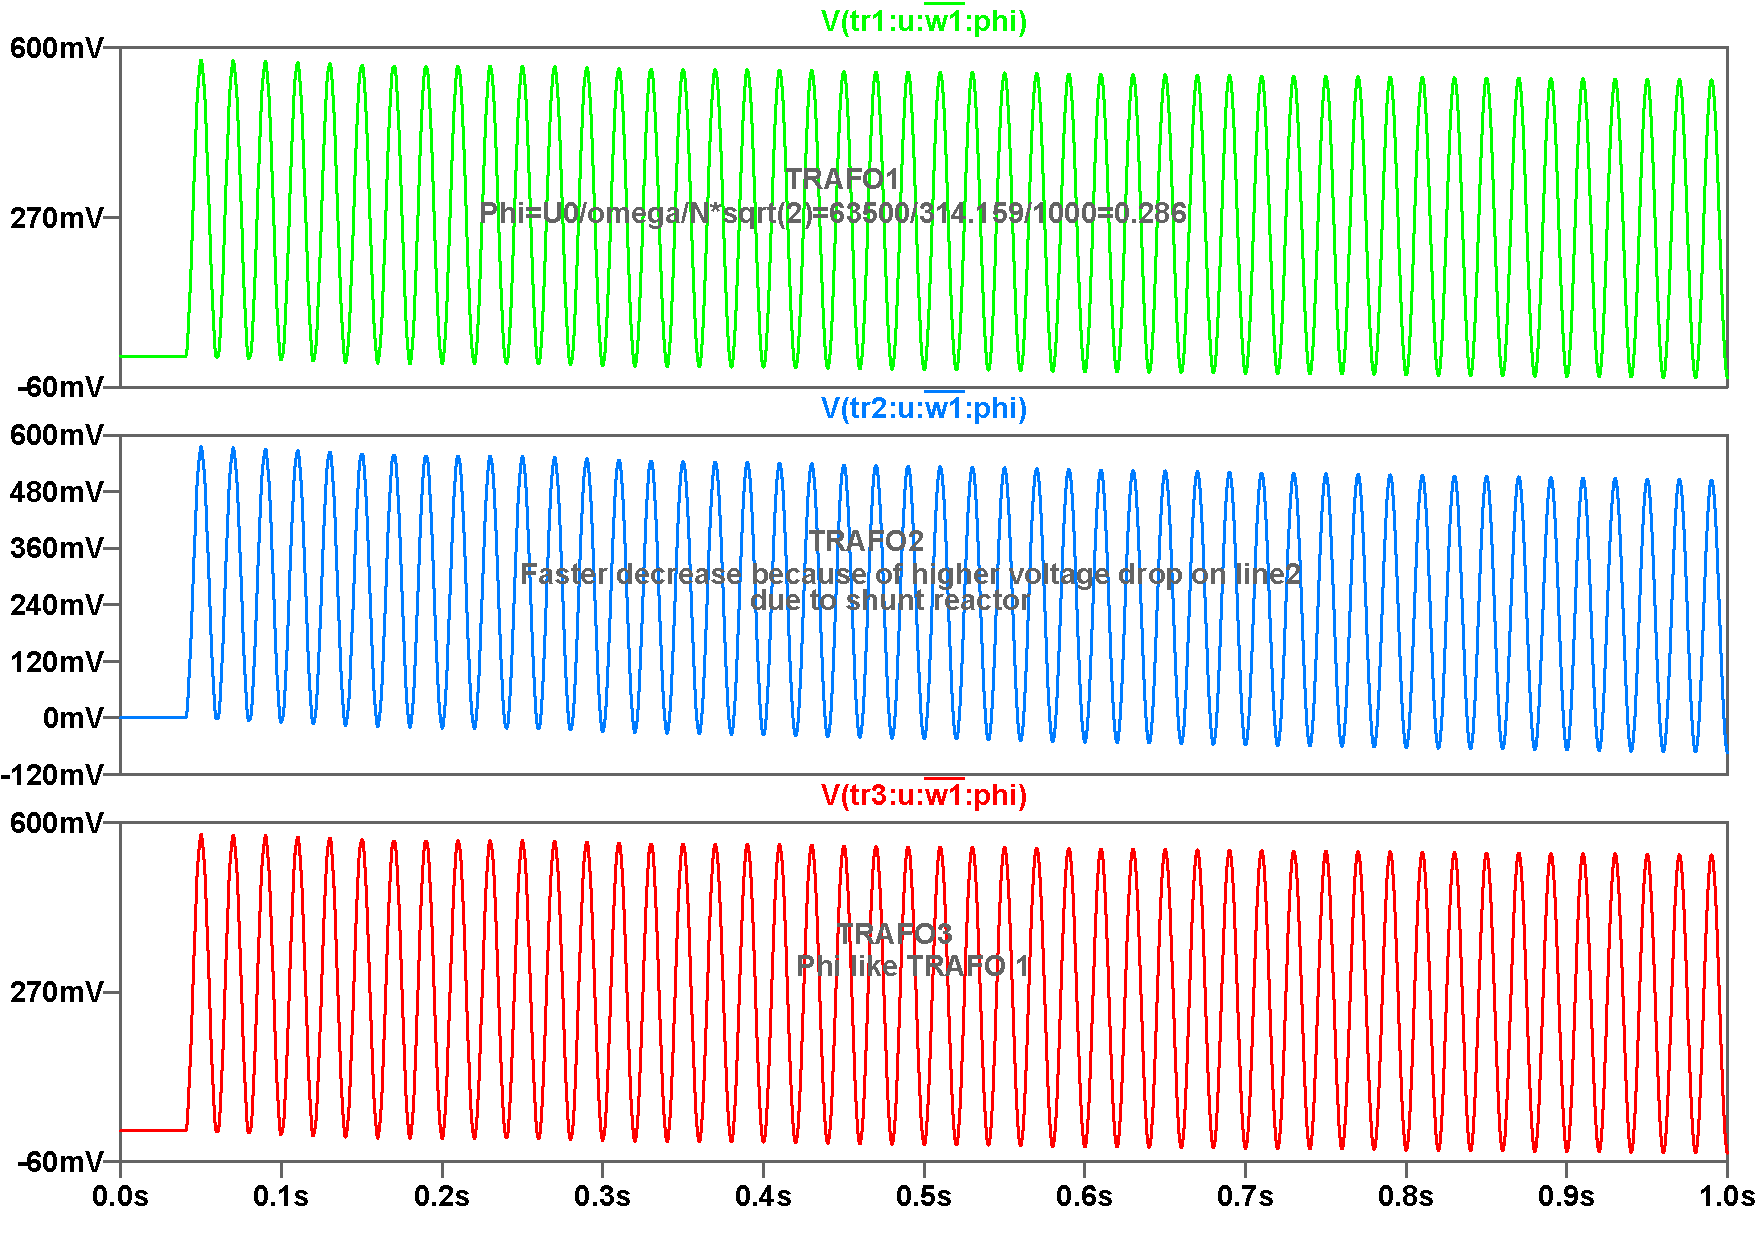
\includegraphics[width=0.90\textwidth]{figures/06_Switching_on_networks/Switching_on_networks_phi-case1}
	\caption{Switching on networks fluxes - case1}
	\label{fig:figure65}
\end{figure}

\begin{figure}[H]
	\centering
	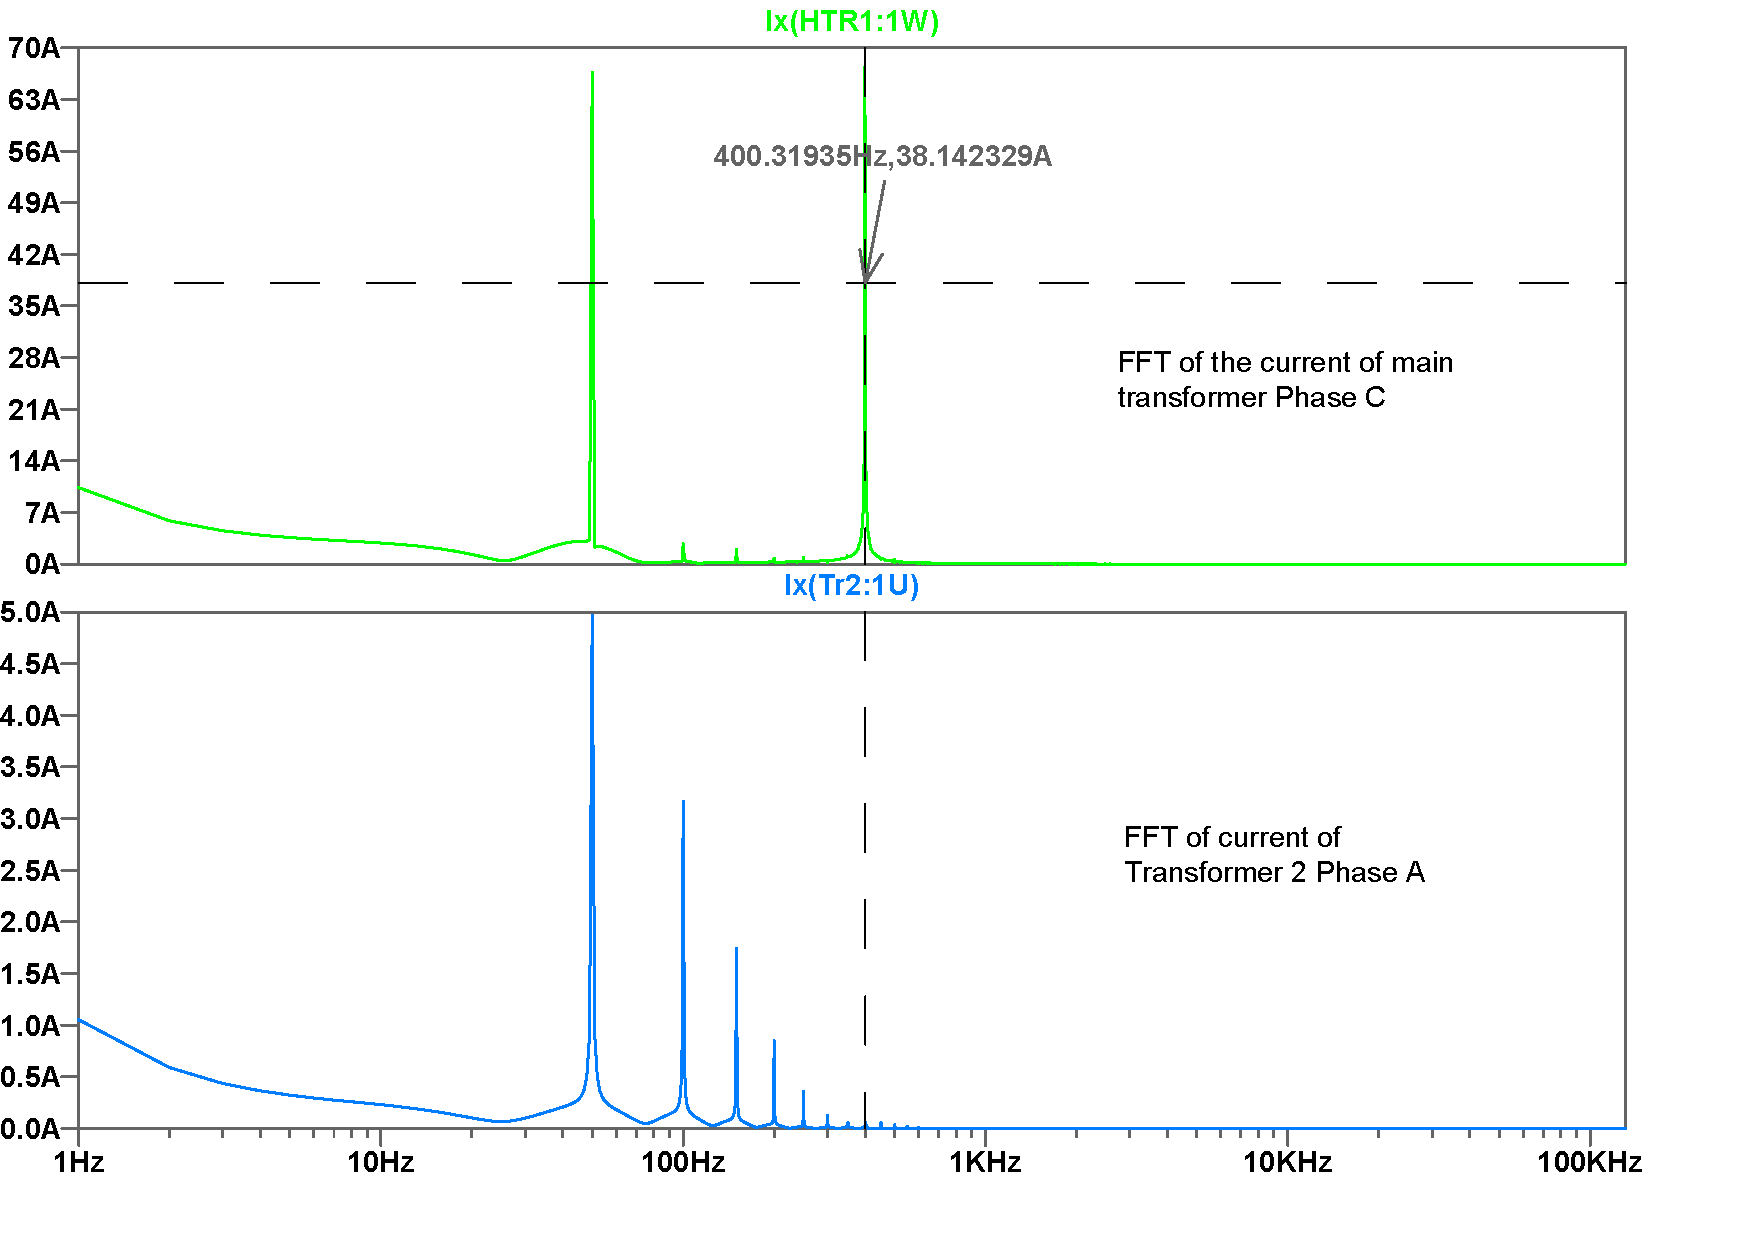
\includegraphics[width=0.90\textwidth]{figures/06_Switching_on_networks/Switching_on_networks_FFT_Transformer-case1}
	\caption{Switching on networks FFT - case1}
	\label{fig:figure66}
\end{figure}

% Measurement values table for the Power System Simulation book.
% Required packages are already loaded by the central preamble:
% booktabs, tabularx, array, siunitx, xcolor.

\begin{table}[htbp]
  \centering
  \caption{Signal ranges for Case 1. All values are peak values, bus values are multiplied by 1.73/1.414}
  \label{tab:measurement-values-case1}
  \small
  \setlength{\tabcolsep}{3.5pt}
  \renewcommand{\arraystretch}{1.18}
  \begin{tabularx}{\textwidth}{@{}
      >{\raggedright\arraybackslash}p{0.055\textwidth}
      >{\raggedright\arraybackslash}p{0.085\textwidth}
      >{\raggedright\arraybackslash}p{0.095\textwidth}
      >{\raggedright\arraybackslash}p{0.105\textwidth}
      >{\raggedright\arraybackslash}p{0.075\textwidth}
      >{\raggedright\arraybackslash}p{0.075\textwidth}
      Y@{}}
    \toprule
    \textbf{Meas.} &
    \textbf{Grid element} &
    \textbf{Phase} &
    \textbf{Voltage level} &
    \textbf{Min.} &
    \textbf{Max.} &
    \textbf{Notes} \\
    \midrule
    $V$ & Bus0  & Ph A       & \SI{220}{\kilo\volt} & \SI{-229}{\kilo\volt} & \SI{229}{\kilo\volt} & -- \\
    $V$ & Bus1  & Ph A & \SI{110}{\kilo\volt} & \SI{-100}{\kilo\volt} & \SI{100}{\kilo\volt} & -- \\
     $V$ & Bus1  & Ph B, C & \SI{110}{\kilo\volt} & \SI{-200}{\kilo\volt} & \SI{200}{\kilo\volt} & -- \\
    $I$ & HTr1  & Ph A       & \SI{220}{\kilo\volt} & \SI{0}{\ampere} & \SI{330}{\ampere} & -- \\
    $I$ & HTr1  & Ph B, C    & \SI{220}{\kilo\volt} & \SI{-540}{\ampere} & \SI{360}{\ampere} & -- \\
    $I$ & KD1   & Ph A       & \SI{110}{\kilo\volt} & \SI{0}{\ampere} & \SI{600}{\ampere} & Steady state: \SI{300}{\ampere} \\
    $I$ & Tr1   & Ph A       & \SI{110}{\kilo\volt} & \SI{-2}{\ampere} & \SI{38}{\ampere} & Due to Petersen values under zero line \\
    $I$ & Tr2   & Ph A       & \SI{110}{\kilo\volt} & \SI{0}{\ampere} & \SI{37}{\ampere} & Due to KD1: faster decrease of current \\
    $I$ & Tr3   & Ph A       & \SI{110}{\kilo\volt} & \SI{0}{\ampere} & \SI{37}{\ampere} & -- \\
    $I$ & Line4 & Ph B, C & \SI{110}{\kilo\volt} & \SI{-3}{\ampere} & \SI{3}{\ampere} & Small capacitive inrush current due to overhead line \\
    $I$ & Line1 & Ph B, C & \SI{110}{\kilo\volt} & \SI{-500}{\ampere} & \SI{500}{\ampere} & High capacitive inrush current due to cable \\
     $I$ & Line1 & Ph A  & \SI{110}{\kilo\volt} & \SI{-100}{\ampere} & \SI{120}{\ampere} & -- \\
     $I$ & Pet1 & Ph N & \SI{110}{\kilo\volt} & \SI{-7}{\ampere} & \SI{7}{\ampere} & Longtime value very small \\
    $V$ & Pet1 & Ph N & \SI{110}{\kilo\volt} & \SI{-1.8}{\kilo\volt} & \SI{1.6}{\kilo\volt} & Longtime value very small \\
    $\Phi$ & Tr1 & Ph A      & \SI{110}{\kilo\volt} & \SI{0}{\weber} & \SI{0.576}{\weber} & Nominal flux: \SI{0.288}{\weber} \\
    FFT & HTr1  & Ph C       & \SI{220}{\kilo\volt} & \SI{50}{\hertz} & \SI{400}{\hertz} & Only \SI{50}{\hertz} and \SI{400}{\hertz} \\
    FFT & Tr2   & Ph A       & \SI{110}{\kilo\volt} & \SI{50}{\hertz} & \SI{250}{\hertz} & \SI{50}{\hertz}, \SI{100}{\hertz}, \SI{150}{\hertz}, \SI{200}{\hertz}, and \SI{250}{\hertz} \\
    \bottomrule
  \end{tabularx}
\end{table}


%\include{chapters/06_Switching Whole Networks/measurement_values.tex}


\section{Case 2: Closing at the Phase-R Voltage Maximum} 
\label{sec:network-closing-voltage-maximum}

Set \texttt{t0=1}. Phase A now closes near its voltage maximum. Its initial
capacitive charging current measured at the primary side of the main transformer is at its maximum, while the magnetising inrush currents of transformers 1, 2 and 3 - because of the corresponding flux - begins close to its natural
steady-state trajectory. Phases B and C contain mixtures of cable-charging and
transformer-magnetizing currents.
The currents of the main transformer 
decay toward steady state within approximately \SI{500}{\milli\second}. The
largest voltage peak occurs in phase A, while phases B and C show similar,
smaller peaks.

The primary currents of the main transformer remain approximately at the level of Case 1. The inrush currents of medium-voltage transformers 1, 2, and 3 are now minimal in Phase A and higher and roughly equal in Phases B and C for transformers 2 and 3, but remain smaller than the inrush currents in Phase A at the switching time t0 = 0. Since the Petsersen current of Transformer 1 becomes quite high at approximately 16 A when t0 = 1, the currents in phases B and C of Transformer 1 differ. The current through the shunt reactor is now symmetrical about zero from the start and is approximately 300 A. The current in Line 1 Phase A is approximately 500 A, and that in Phases B and C is approximately 300 A. The magnetic flux in phases B and C is now at its highest, but not as high as it was in Phase A in Case 1. Therefore the inrush currents of Phase B and C are smaller than those in phase A of Case 1.
NOTE: Due to the highly nonlinear magnetic characteristic curve, small changes in the flux values cause large changes in the magnetization currents.  
For Waveforms see figures \ref{fig:figure67}-\ref{fig:figure610}. 
For Measurement values and signal ranges see table: \ref{tab:measurement-values-case2}.\\

\begin{figure}[H]
	\centering
	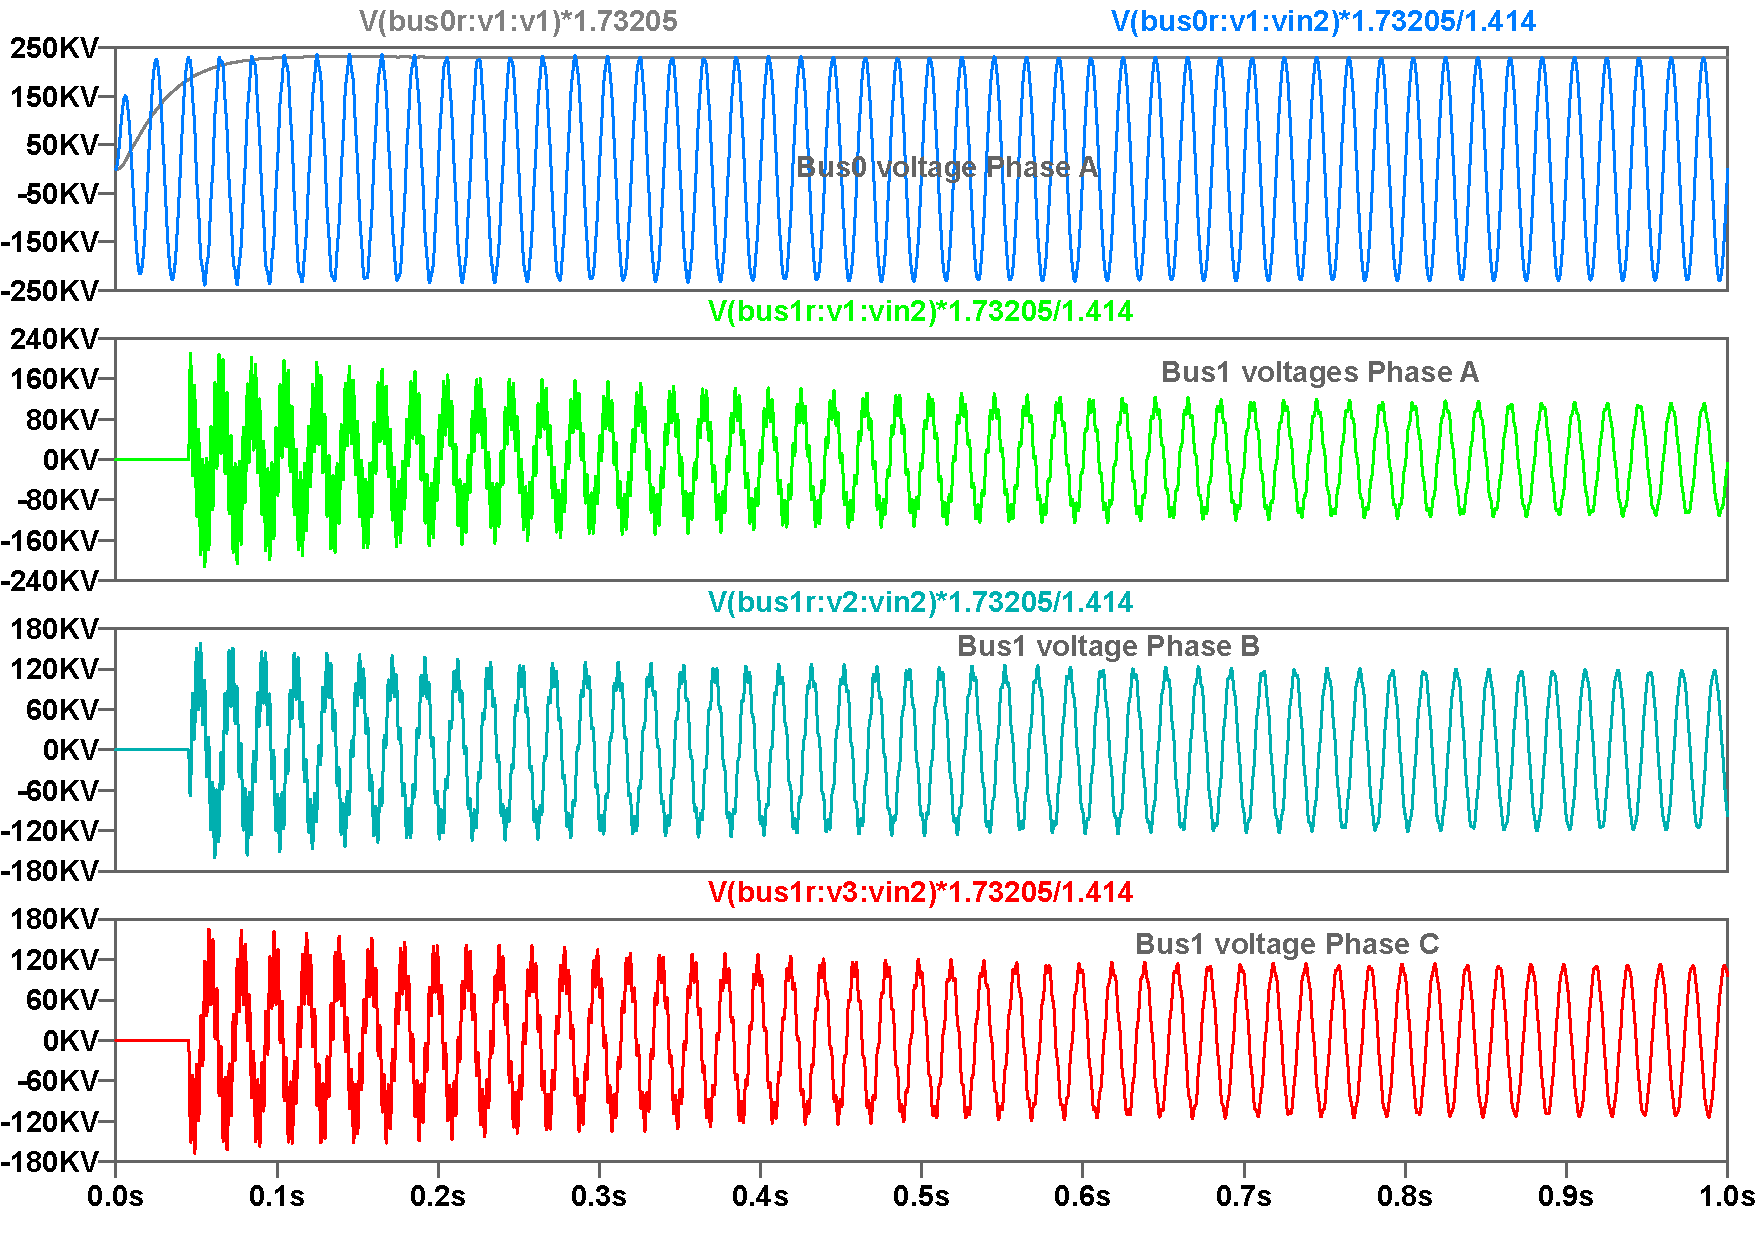
\includegraphics[width=0.90\textwidth]{figures/06_Switching_on_networks/Switching_on_networks_Bus0_Bus1_voltages-case2}
	\caption{Switching on networks voltages - case2}
	\label{fig:figure67}
\end{figure}

\begin{figure}[H]
	\centering
	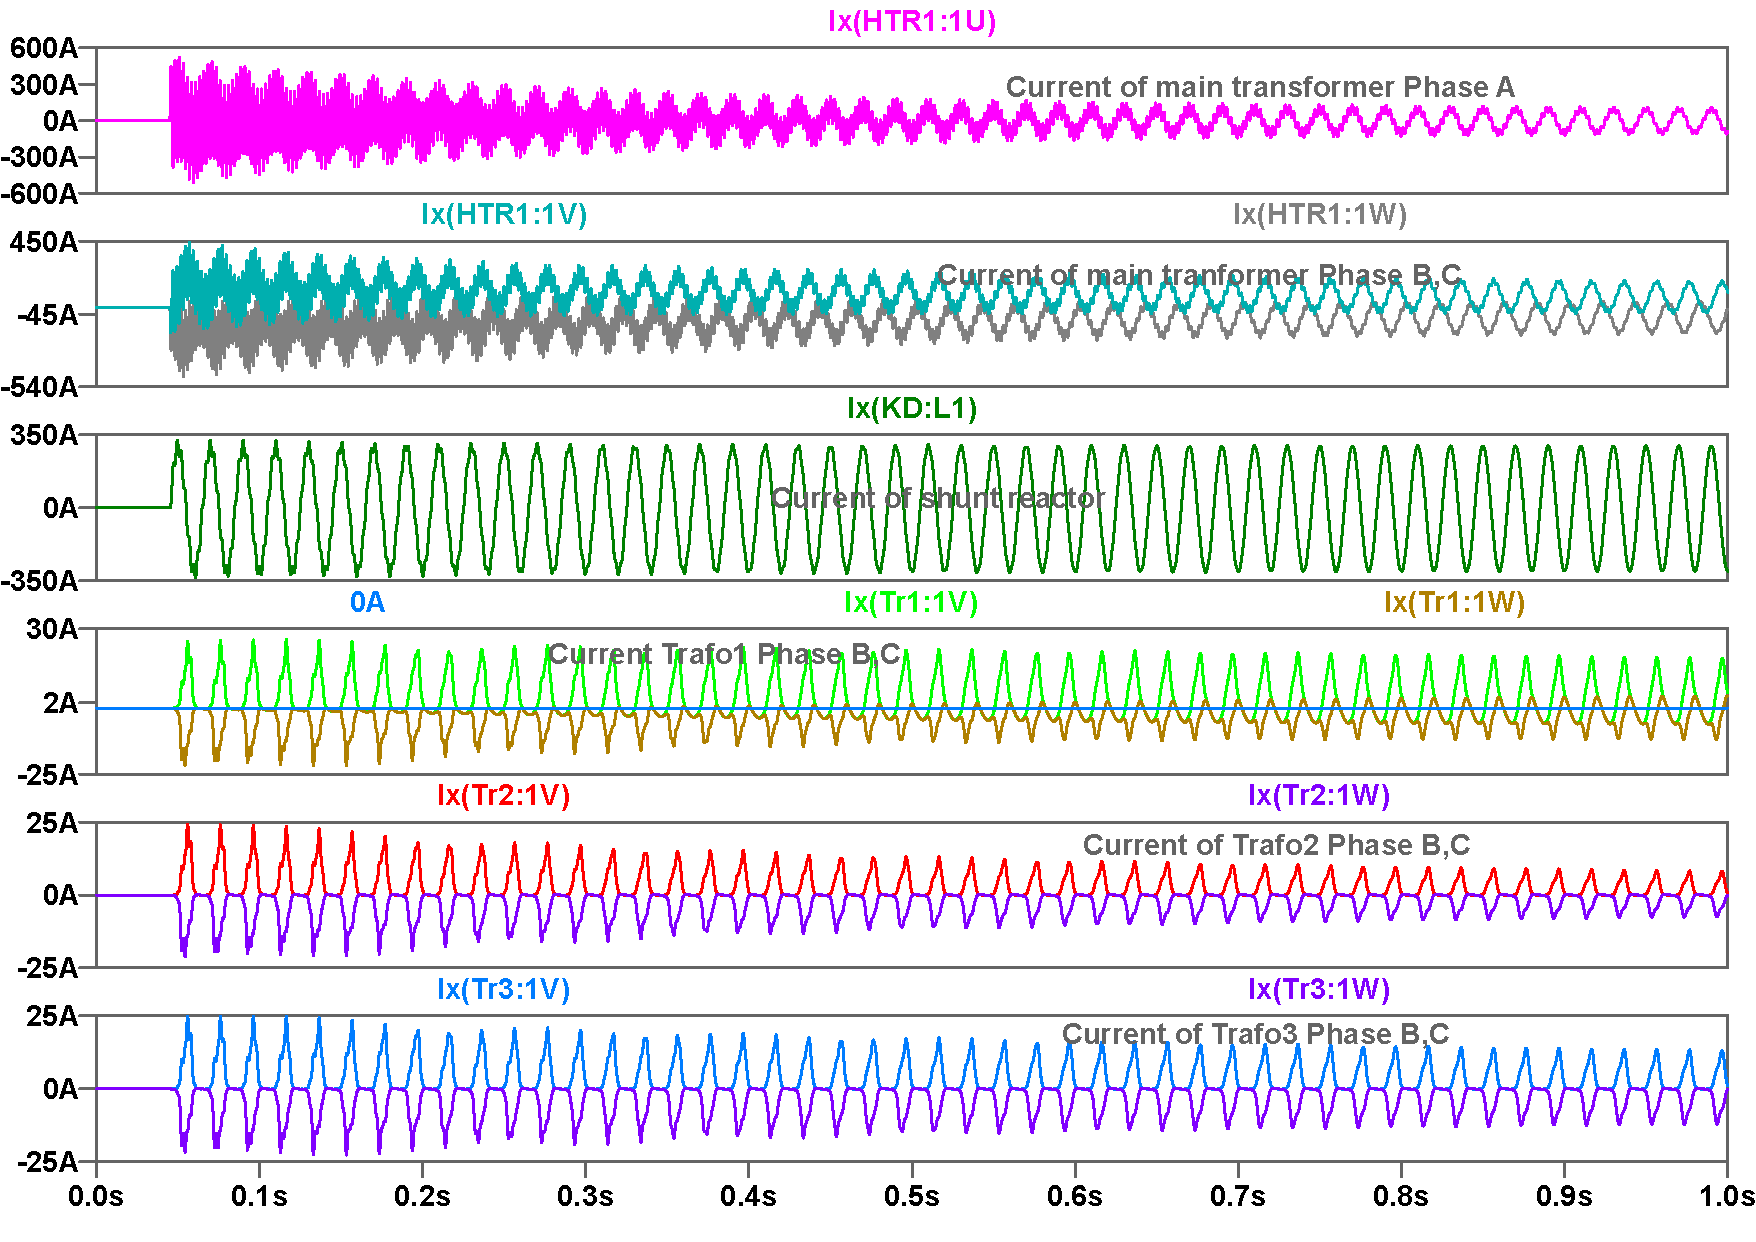
\includegraphics[width=0.90\textwidth]{figures/06_Switching_on_networks/Switching_on_networks_currents-case2}
	\caption{Switching on networks currents - case2}
	\label{fig:figure68}
\end{figure}

\begin{figure}[H]
	\centering
	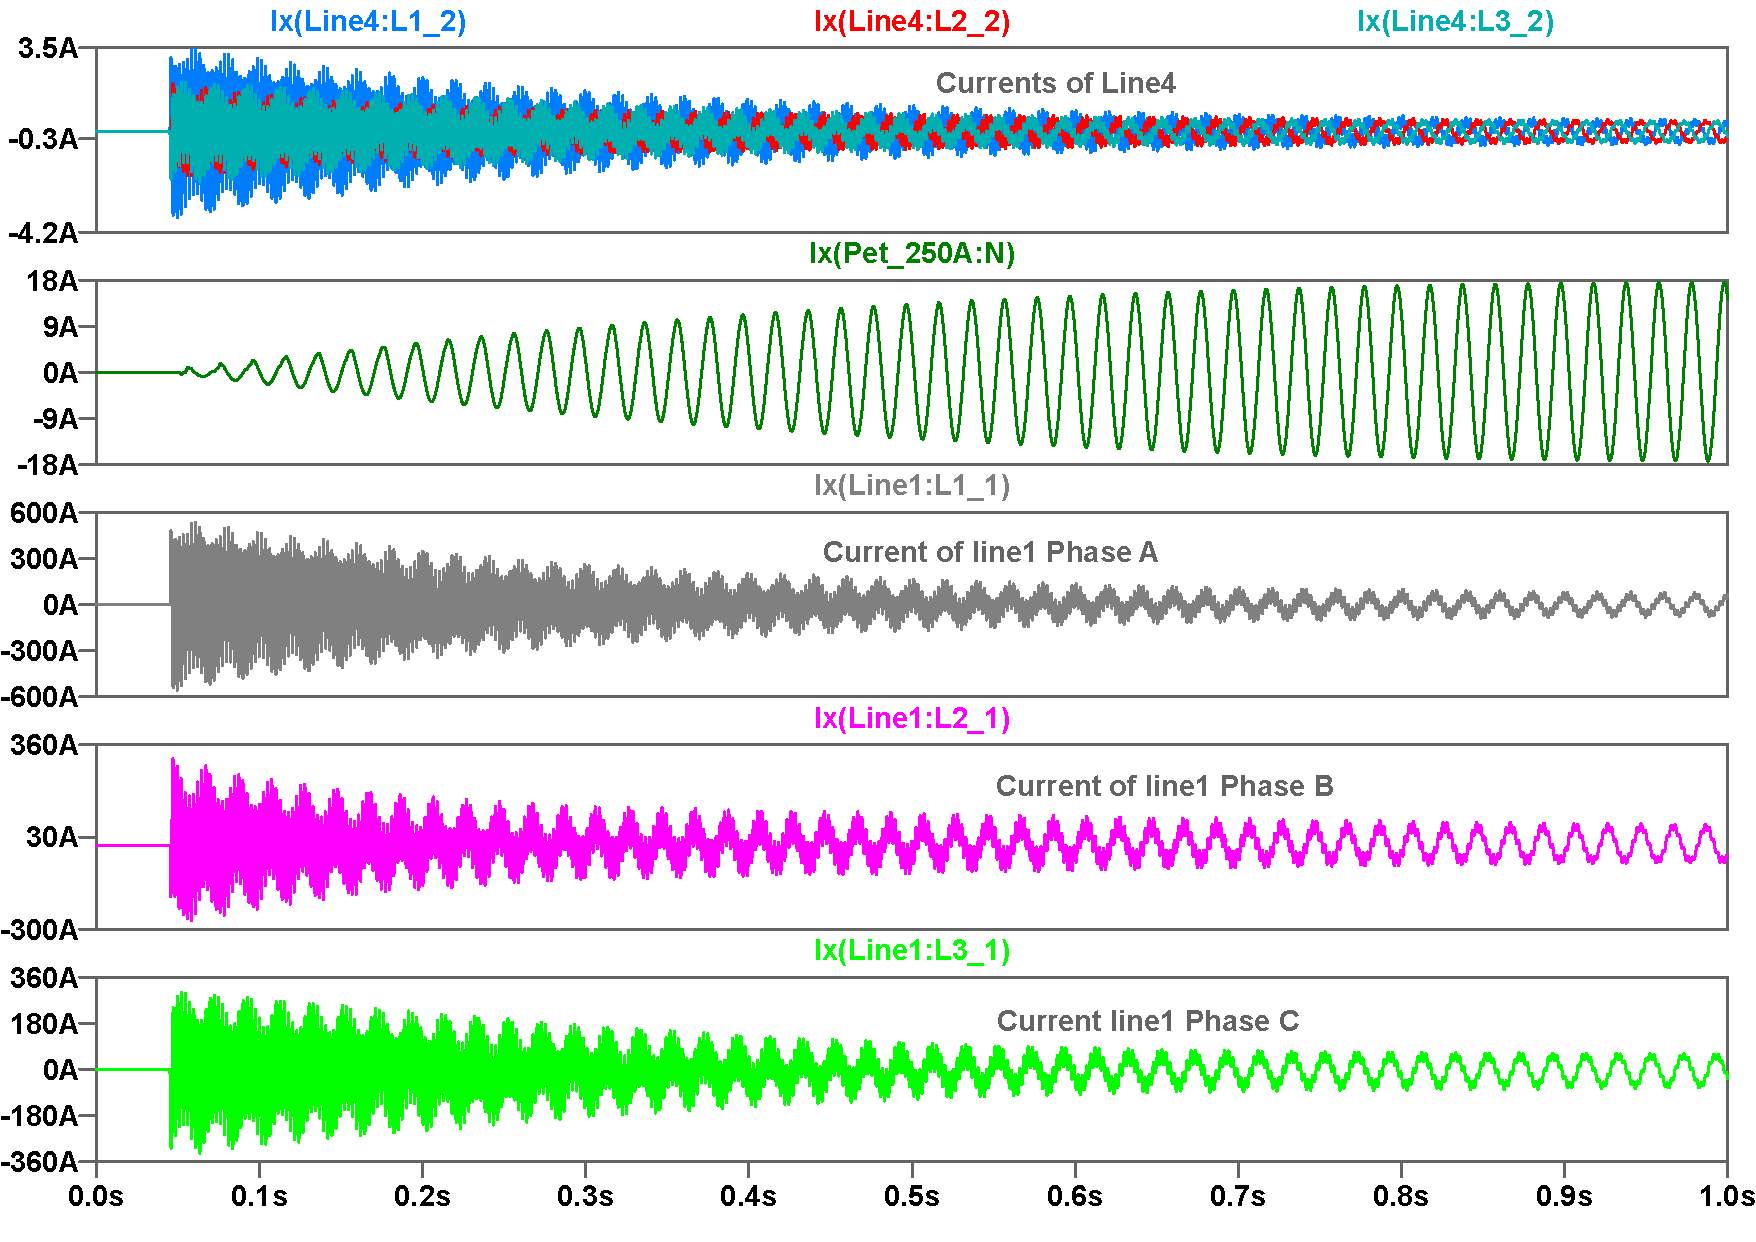
\includegraphics[width=0.90\textwidth]{figures/06_Switching_on_networks/Switching_on_networks_currents_Line1_Line4-case2}
	\caption{Switching on networks currents line1, line4 - case2}
	\label{fig:figure69}
\end{figure}

\begin{figure}[H]
	\centering
	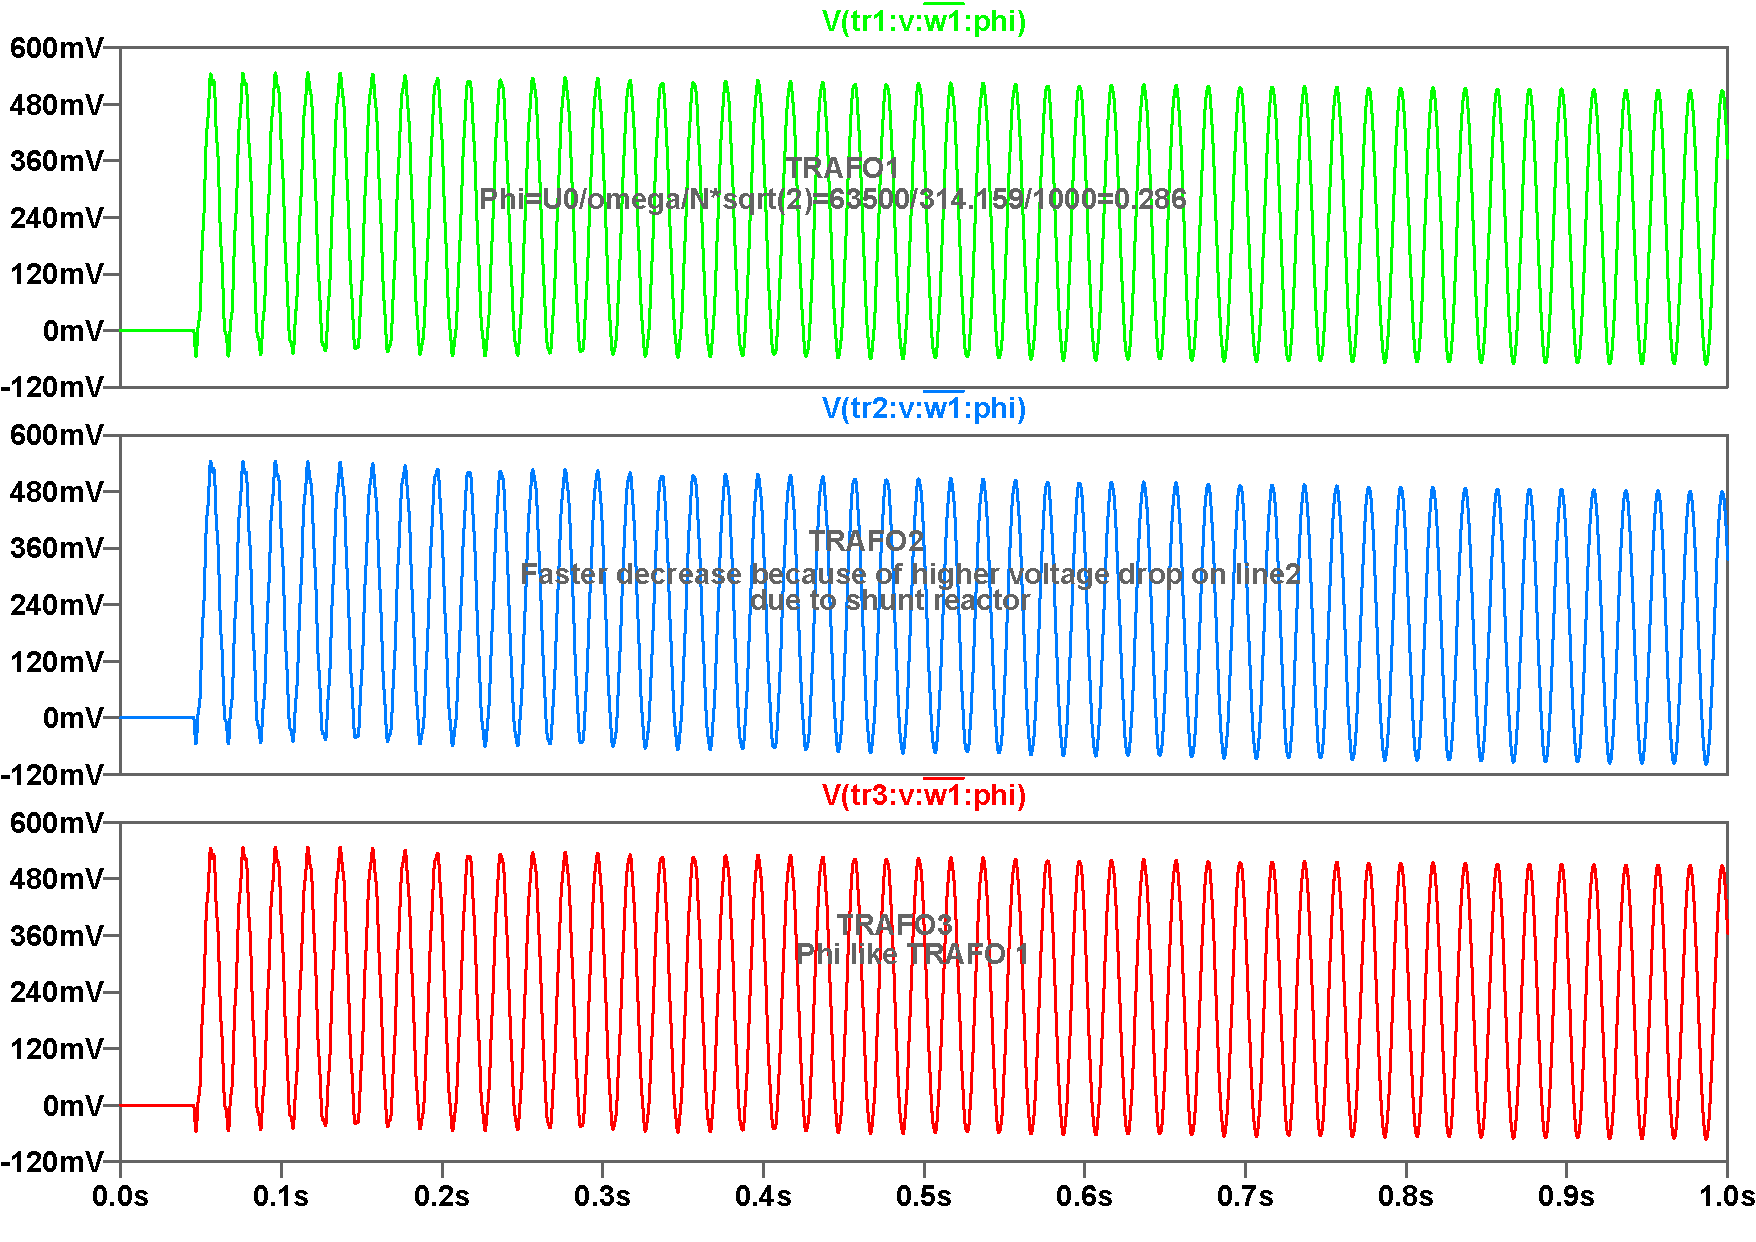
\includegraphics[width=0.90\textwidth]{figures/06_Switching_on_networks/Switching_on_networks_phi-case2}
	\caption{Switching on networks fluxes - case2}
	\label{fig:figure610}
\end{figure}

% Measurement values table for the Power System Simulation book.
% Required packages are already loaded by the central preamble:
% booktabs, tabularx, array, siunitx, xcolor.

\begin{table}[htbp]
  \centering
  \caption{Signal ranges for Case 2. All values are peak values, bus values are multiplied by 1.73/1.414}
  \label{tab:measurement-values-case2}
  \small
  \setlength{\tabcolsep}{3.5pt}
  \renewcommand{\arraystretch}{1.18}
  \begin{tabularx}{\textwidth}{@{}
      >{\raggedright\arraybackslash}p{0.055\textwidth}
      >{\raggedright\arraybackslash}p{0.085\textwidth}
      >{\raggedright\arraybackslash}p{0.095\textwidth}
      >{\raggedright\arraybackslash}p{0.105\textwidth}
      >{\raggedright\arraybackslash}p{0.075\textwidth}
      >{\raggedright\arraybackslash}p{0.075\textwidth}
      Y@{}}
    \toprule
    \textbf{Meas.} &
    \textbf{Grid element} &
    \textbf{Phase} &
    \textbf{Voltage level} &
    \textbf{Min.} &
    \textbf{Max.} &
    \textbf{Notes} \\
    \midrule
    $V$ & Bus0  & Ph A       & \SI{220}{\kilo\volt} & \SI{-229}{\kilo\volt} & \SI{229}{\kilo\volt} & -- \\
    $V$ & Bus1  & Ph A, B, C & \SI{110}{\kilo\volt} & \SI{-200}{\kilo\volt} & \SI{200}{\kilo\volt} & -- \\
    $I$ & HTr1  & Ph A       & \SI{220}{\kilo\volt} & \SI{-520}{\ampere} & \SI{510}{\ampere} & -- \\
    $I$ & HTr1  & Ph B       & \SI{220}{\kilo\volt} & \SI{-170}{\ampere} & \SI{460}{\ampere} & -- \\
    $I$ & HTr1  & Ph C       & \SI{220}{\kilo\volt} & \SI{-470}{\ampere} & \SI{180}{\ampere} & -- \\
    $I$ & KD1   & Ph A       & \SI{110}{\kilo\volt} & \SI{-300}{\ampere} & \SI{300}{\ampere} & Steady state: \SI{300}{\ampere} \\
    $I$ & Tr1   & Ph B       & \SI{110}{\kilo\volt} & \SI{-4}{\ampere} & \SI{26}{\ampere} & Due to Petersen values under zero line \\
    $I$ & Tr2   & Ph B       & \SI{110}{\kilo\volt} & \SI{0}{\ampere} & \SI{25}{\ampere} & Due to KD: faster decrease of current \\
    $I$ & Tr3   & Ph A      & \SI{110}{\kilo\volt} & \SI{0}{\ampere} & \SI{25}{\ampere} & -- \\
    $I$ & Line4 & Ph A & \SI{110}{\kilo\volt} & \SI{-3.5}{\ampere} & \SI{3.5}{\ampere} & Small capacitive inrush current due to overhead line \\
    $I$ & Line1 & Ph A & \SI{110}{\kilo\volt} & \SI{-500}{\ampere} & \SI{500}{\ampere} & High capacitive inrush current due to cable \\
    $I$ & Line1 & Ph B, C & \SI{110}{\kilo\volt} & \SI{-300}{\ampere} & \SI{300}{\ampere} & High capacitive inrush current due to cable \\
    $I$ & Pet1 & Ph N & \SI{110}{\kilo\volt} & \SI{-18}{\ampere} & \SI{18}{\ampere} & Longtime value very small \\
    $V$ & Pet1 & Ph N & \SI{110}{\kilo\volt} & \SI{-4.5}{\kilo\volt} & \SI{4.5}{\kilo\volt} & Longtime value very small \\
    $\Phi$ & Tr1 & Ph B, C   & \SI{110}{\kilo\volt} & \SI{0}{\weber} & \SI{0.54}{\weber} & Nominal flux: \SI{0.288}{\weber} \\
    \bottomrule
  \end{tabularx}
\end{table}



\section{Case 3: Closing at Voltage Zero with Full Residual Flux}
\label{sec:network-closing-residual-flux}

Set \texttt{psi\_0=1}. Phase A then carries a very large combined magnetizing
current from the medium-voltage transformers. Measured on the
\SI{220}{\kilo\volt} side of the main transformer, the peak is approximately
\SI{920}{\ampere}. This exceeds the rated peak current of
approximately $\sqrt{2}\cdot\SI{525}{\ampere}=\SI{742}{\ampere}$.

With unfavourable full residual flux, the Phase A flux can theoretically approach three times its normal peak. The theoretical peak would therefore be approximately \SI{8.64}{\weber}.
This theoretical peak cannot be achieved in practice. The reason is, on the one hand, the reduced voltage caused by the high current and external and internal voltage drops. The attainable flux is reduced by voltage drops caused by the high current, as well as by secondary-winding currents and leakage flux. 
The fast decrease of the currents is due to the nonlinear characteristic of the magnetizing curve. 

The neutral-point voltage across the Petersen coil of transformer 1 initially rises to a high value (about nominal voltage) and then
decays slowly. The cause is the large asymmetry of the phase magnetizing
currents, which also makes the phase-to-earth voltages asymmetric. The
line-to-line voltages are much less affected. If the simulation is extended to
\SI{60}{\second}, the magnetizing currents approach their small steady-state
values and the Petersen-coil voltage settles to approximately
\SIrange{1}{2}{\kilo\volt}.

The very high neutral displacement voltage, which reaches approximately the nominal phase-to-earth voltage, which also slowly builds up at the neutral point of the main transformer, causes a highly asymmetrical voltage in Phase B of the grid. This voltage first rises, then drops to nearly half the rated voltage, and then rises again. 

For Waveforms see figures \ref{fig:figure611}-\ref{fig:figure614}. 
For Measurement values and signal ranges see table: \ref{tab:measurement-values-case3}.\\ 

\begin{figure}[H]
	\centering
	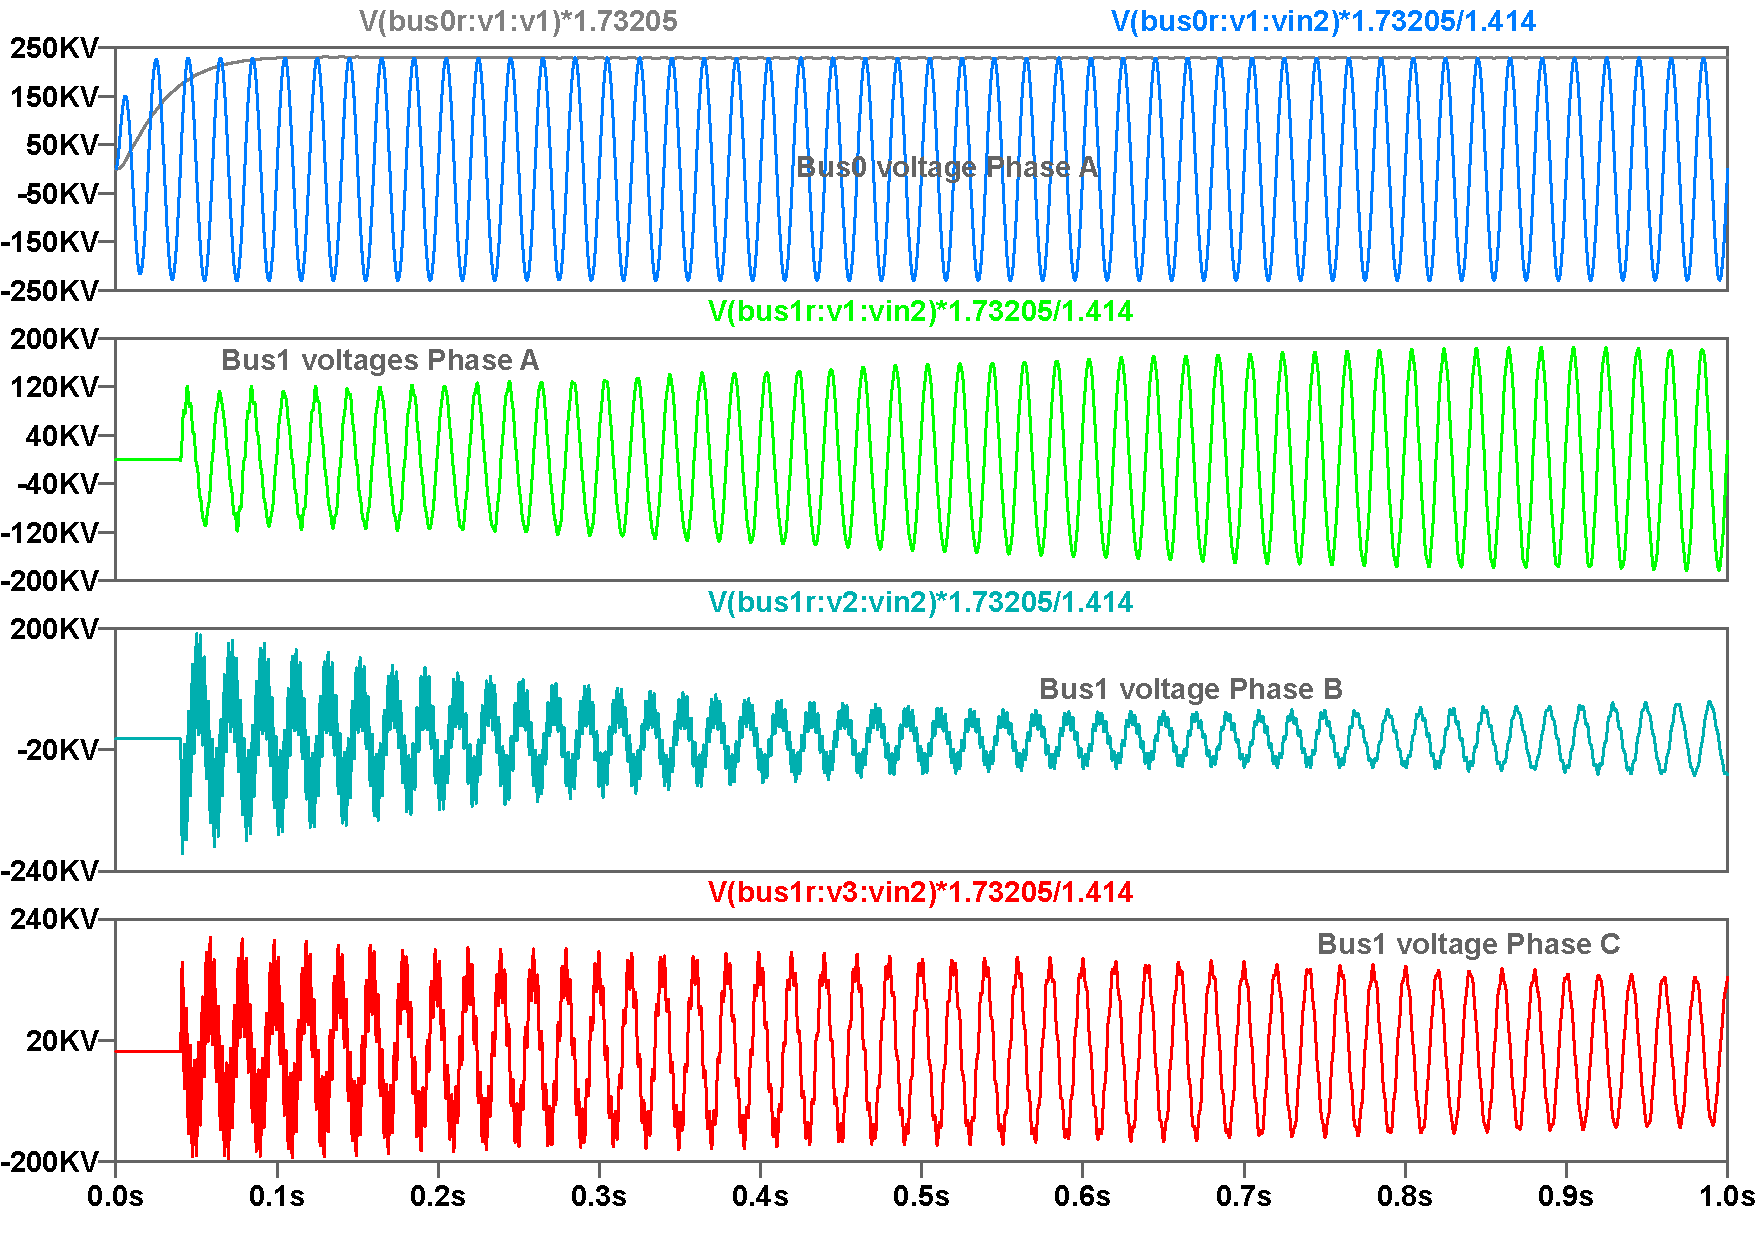
\includegraphics[width=0.90\textwidth]{figures/06_Switching_on_networks/Switching_on_networks_Bus0_Bus1_voltages-case3}
	\caption{Switching on networks voltages - case3}
	\label{fig:figure611}
\end{figure}

\begin{figure}[H]
	\centering
	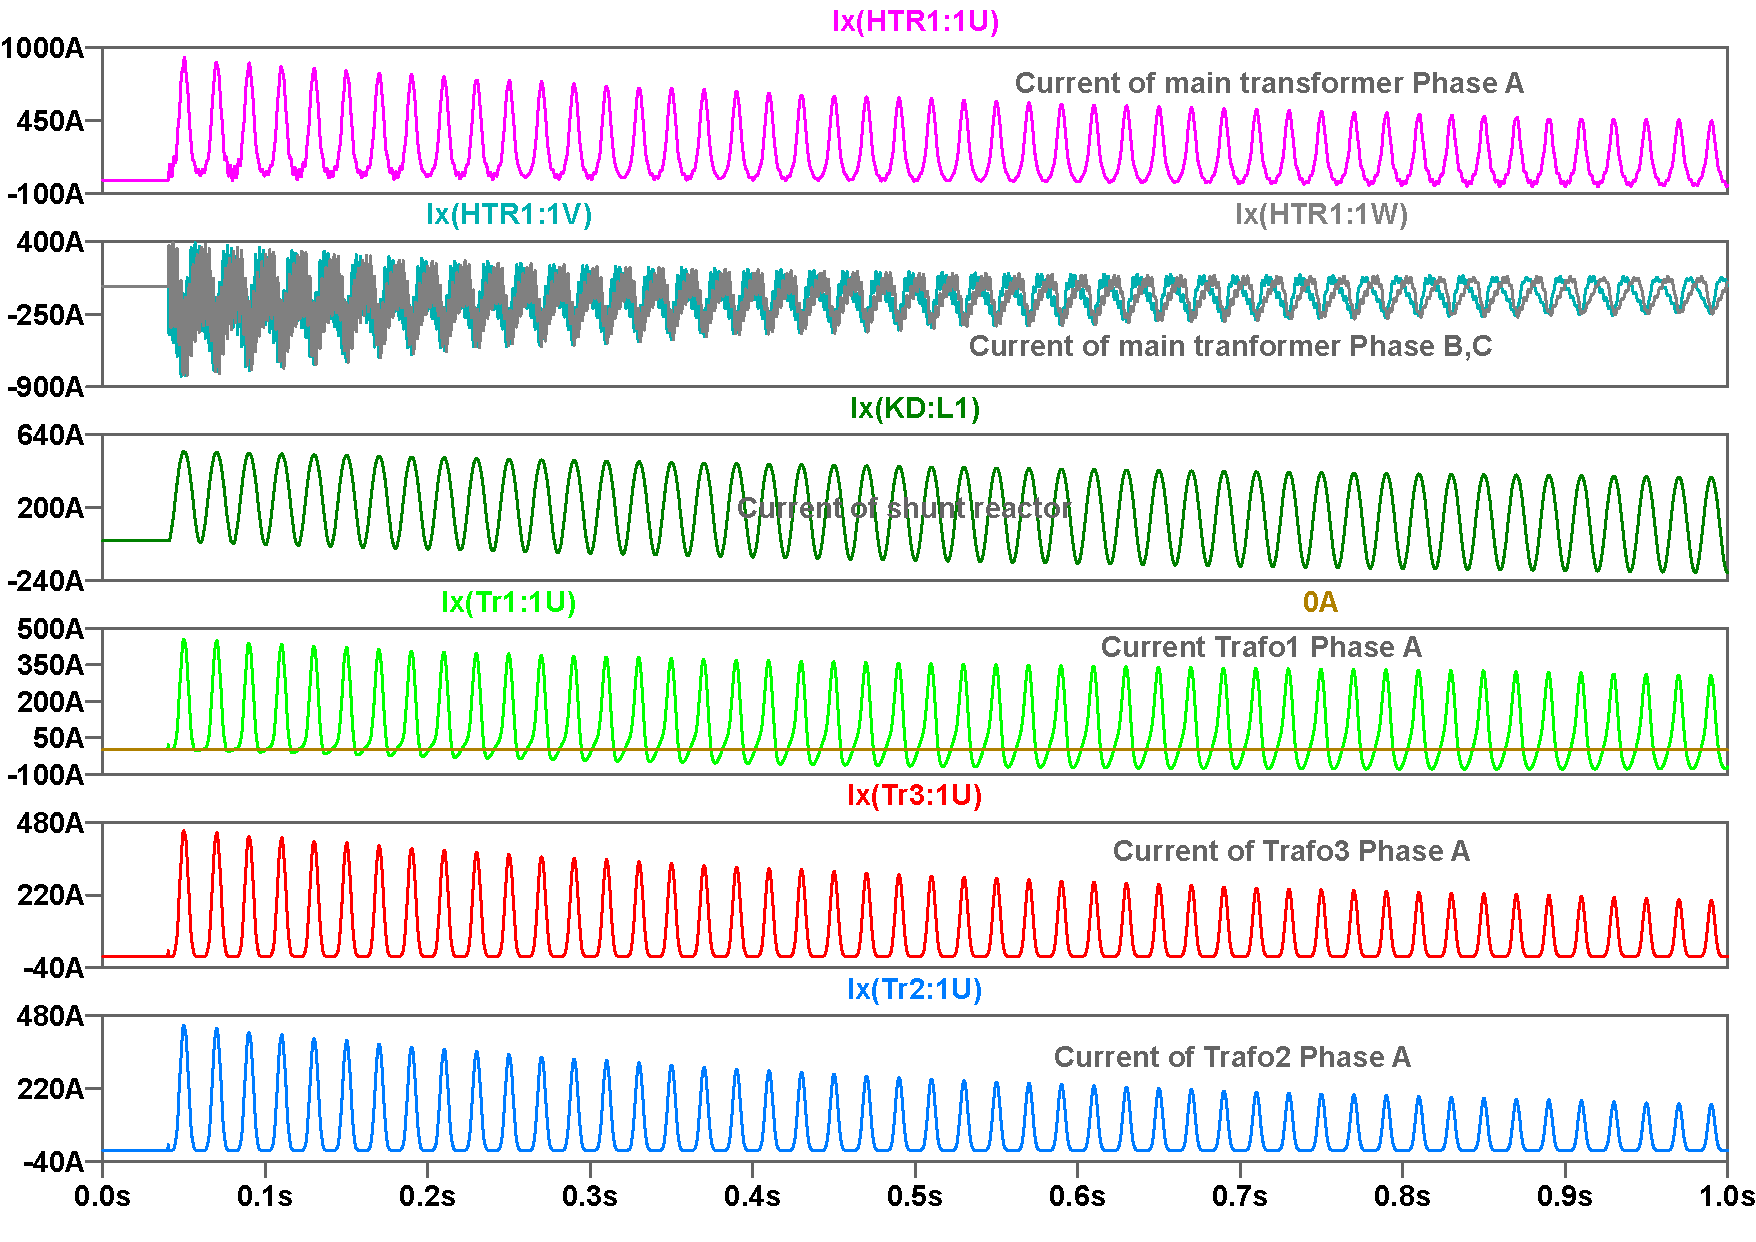
\includegraphics[width=0.90\textwidth]{figures/06_Switching_on_networks/Switching_on_networks_currents-case3}
	\caption{Switching on networks currents - case3}
	\label{fig:figure612}
\end{figure}

\begin{figure}[H]
	\centering
	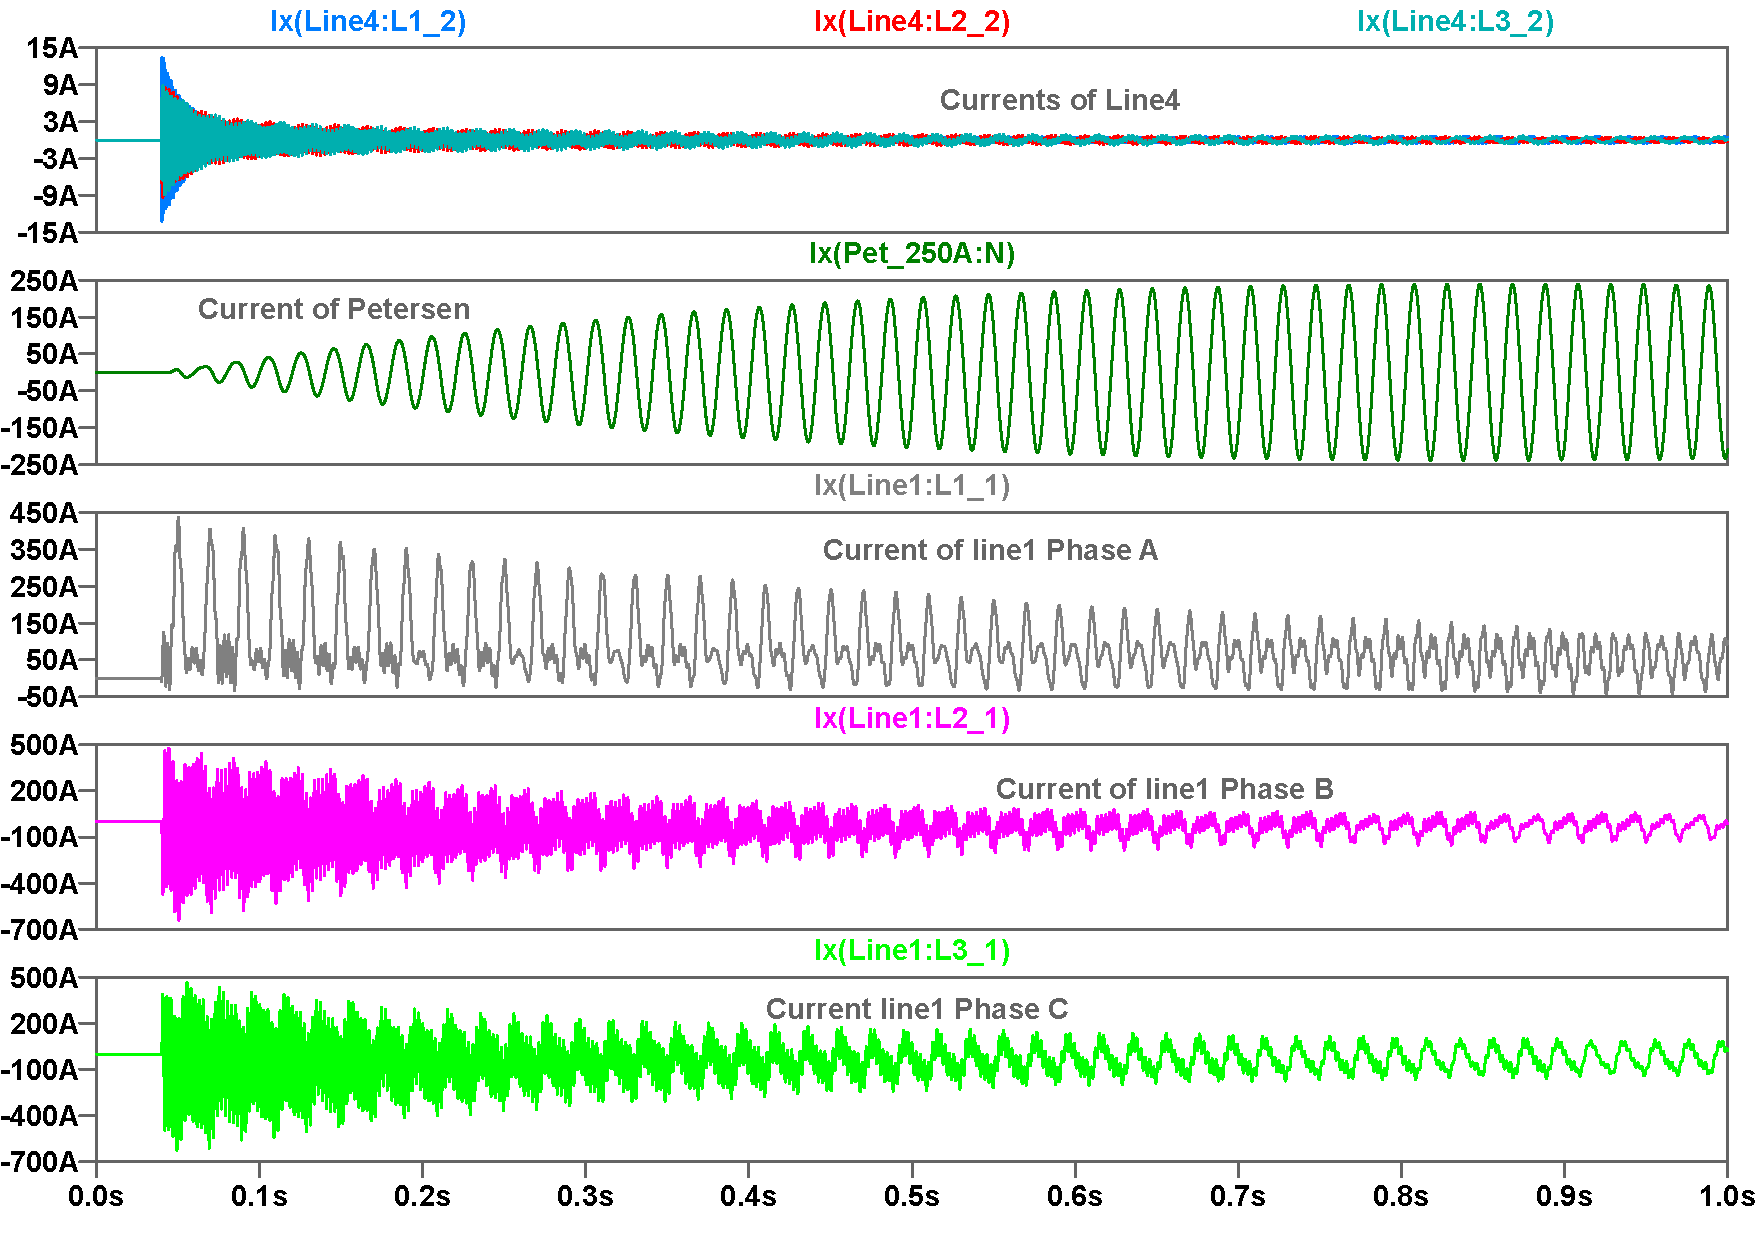
\includegraphics[width=0.90\textwidth]{figures/06_Switching_on_networks/Switching_on_networks_currents_Line1_Line4-case3}
	\caption{Switching on networks currents line1, line4 - case3}
	\label{fig:figure613}
\end{figure}

\begin{figure}[H]
	\centering
	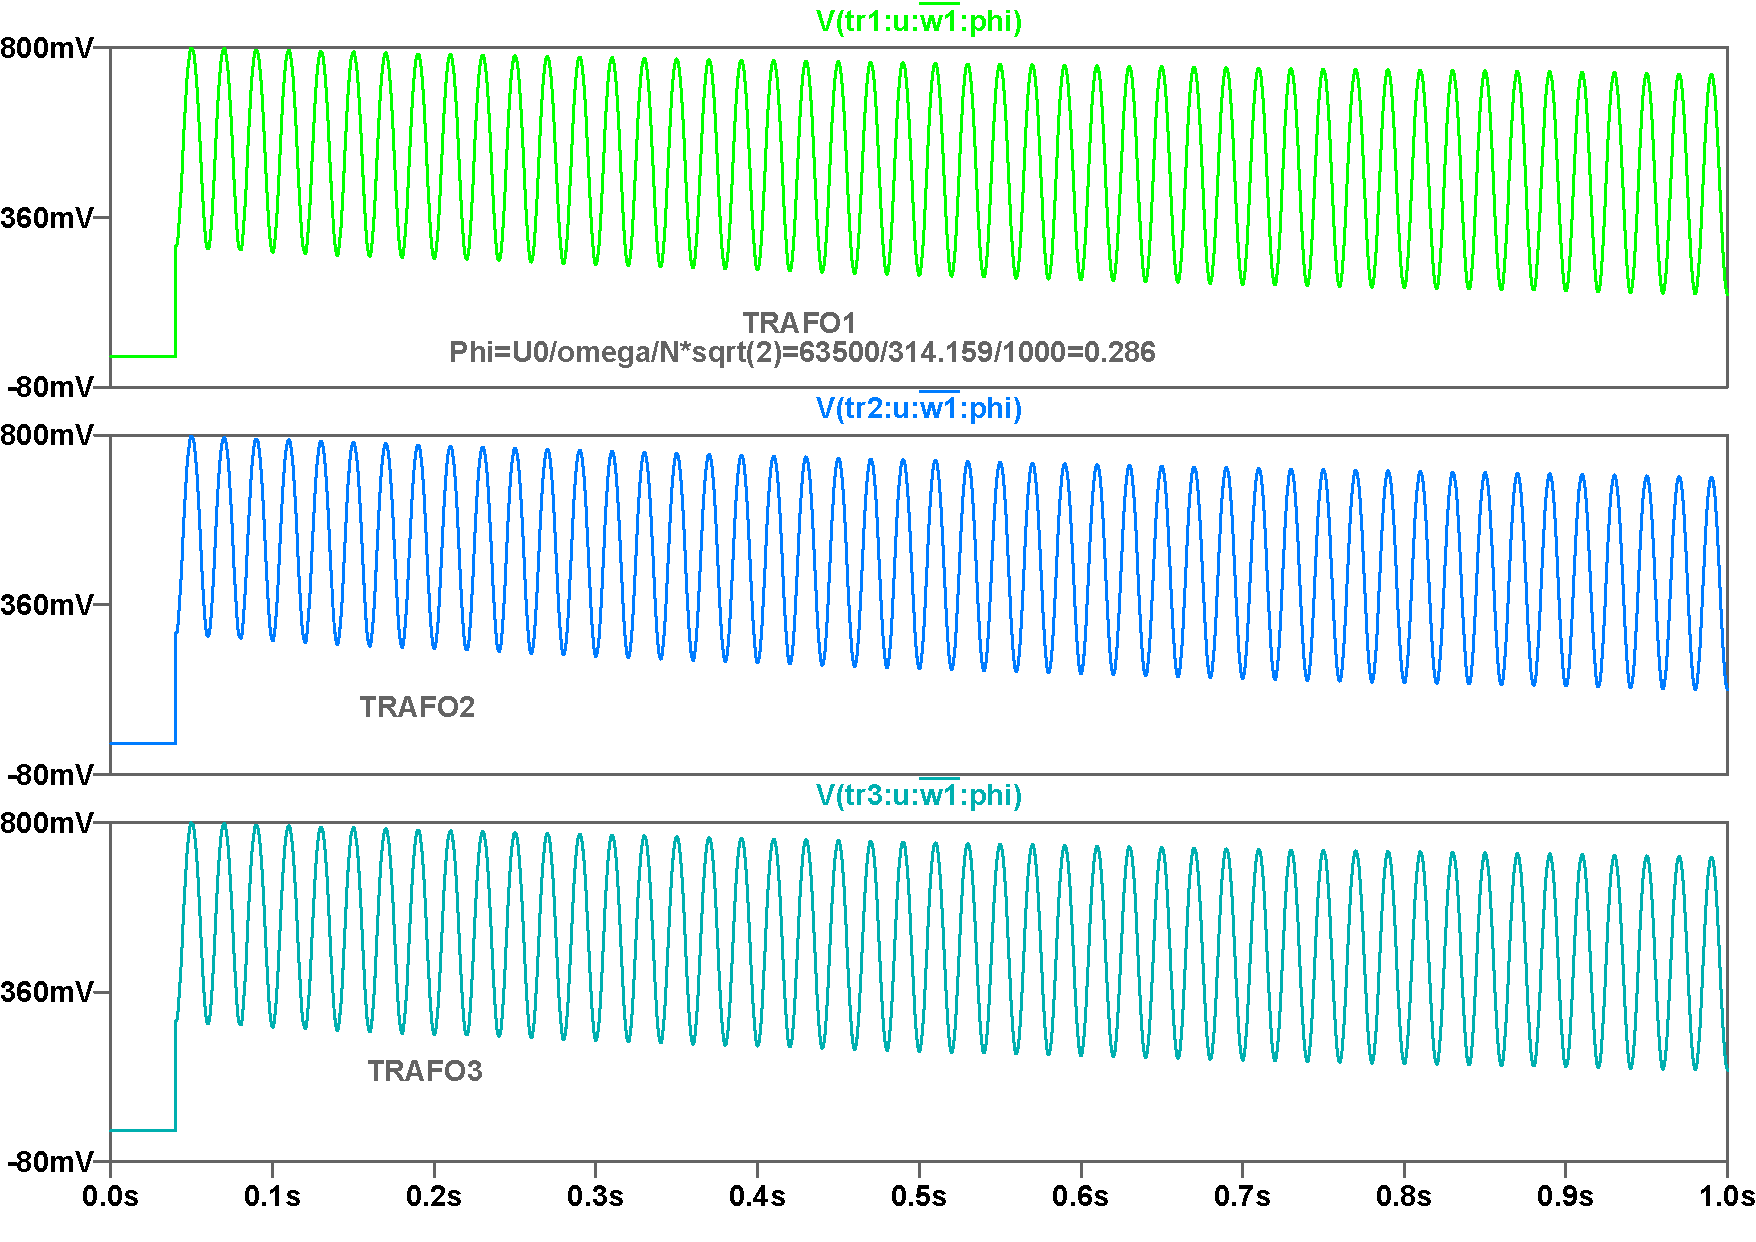
\includegraphics[width=0.90\textwidth]{figures/06_Switching_on_networks/Switching_on_networks_phi-case3}
	\caption{Switching on networks fluxes - case3}
	\label{fig:figure614}
\end{figure}

% Measurement values table for the Power System Simulation book.
% Required packages are already loaded by the central preamble:
% booktabs, tabularx, array, siunitx, xcolor.

\begin{table}[htbp]
  \centering
  \caption{Signal ranges for Case 3. All values are peak values, bus values are multiplied by 1.73/1.414}
  \label{tab:measurement-values-case3}
  \small
  \setlength{\tabcolsep}{3.5pt}
  \renewcommand{\arraystretch}{1.18}
  \begin{tabularx}{\textwidth}{@{}
      >{\raggedright\arraybackslash}p{0.055\textwidth}
      >{\raggedright\arraybackslash}p{0.085\textwidth}
      >{\raggedright\arraybackslash}p{0.095\textwidth}
      >{\raggedright\arraybackslash}p{0.105\textwidth}
      >{\raggedright\arraybackslash}p{0.075\textwidth}
      >{\raggedright\arraybackslash}p{0.075\textwidth}
      Y@{}}
    \toprule
    \textbf{Meas.} &
    \textbf{Grid element} &
    \textbf{Phase} &
    \textbf{Voltage level} &
    \textbf{Min.} &
    \textbf{Max.} &
    \textbf{Notes} \\
    \midrule
    $V$ & Bus0  & Ph A       & \SI{220}{\kilo\volt} & \SI{-229}{\kilo\volt} & \SI{229}{\kilo\volt} & -- \\
    $V$ & Bus1  & Ph A,    & \SI{110}{\kilo\volt} & \SI{-120}{\kilo\volt} & \SI{120}{\kilo\volt} & Startup values low and later higher \\
    $V$ & Bus1  & Ph B     & \SI{110}{\kilo\volt} & \SI{-200}{\kilo\volt} & \SI{200}{\kilo\volt} & Startup values high and later much smaller than higher again, Steady state: \SI{114}{\kilo\volt} \\
    $V$ & Bus1  & Ph C     & \SI{110}{\kilo\volt} & \SI{-200}{\kilo\volt} & \SI{200}{\kilo\volt} & Steady state: \SI{114}{\kilo\volt} RMS \\
    $I$ & HTr1  & Ph A       & \SI{220}{\kilo\volt} & \SI{0}{\ampere} & \SI{920}{\ampere} & -- \\
    $I$ & HTr1  & Ph B       & \SI{220}{\kilo\volt} & \SI{-800}{\ampere} & \SI{400}{\ampere} & -- \\
    $I$ & HTr1  & Ph C       & \SI{220}{\kilo\volt} & \SI{-800}{\ampere} & \SI{400}{\ampere} & -- \\
    $I$ & KD1   & Ph A       & \SI{110}{\kilo\volt} & \SI{0}{\ampere} & \SI{540}{\ampere} & Steady state: \SI{300}{\ampere} \\
    $I$ & Tr1   & Ph A       & \SI{110}{\kilo\volt} & \SI{-80}{\ampere} & \SI{450}{\ampere} & Due to Petersen values under zero line \\
    $I$ & Tr2   & Ph A       & \SI{110}{\kilo\volt} & \SI{0}{\ampere} & \SI{450}{\ampere} & Due to KD1: faster decrease of current \\
    $I$ & Tr3   & Ph A      & \SI{110}{\kilo\volt} & \SI{0}{\ampere} & \SI{450}{\ampere} & -- \\
    $I$ & Line4 & Ph A & \SI{110}{\kilo\volt} & \SI{-13}{\ampere} & \SI{13}{\ampere} & Small capacitive inrush current  \\
    $I$ & Line1 & Ph A & \SI{110}{\kilo\volt} & \SI{-20}{\ampere} & \SI{440}{\ampere} & High capacitive inrush current due to cable \\
    $I$ & Line1 & Ph B, C & \SI{110}{\kilo\volt} & \SI{-500}{\ampere} & \SI{500}{\ampere} & High capacitive inrush current due to cable \\
    $I$ & Pet1 & Ph N & \SI{110}{\kilo\volt} & \SI{-240}{\ampere} & \SI{240}{\ampere} & Longtime value very small \\
    $V$ & Pet1 & Ph N & \SI{110}{\kilo\volt} & \SI{-60}{\kilo\volt} & \SI{60}{\kilo\volt} & Longtime value very small \\
    $\Phi$ & Tr1 & Ph A, B, C   & \SI{110}{\kilo\volt} & \SI{0}{\weber} & \SI{0.8}{\weber} & Nominal flux: \SI{0.288}{\weber} \\
    \bottomrule
  \end{tabularx}
\end{table}


\section{Case 4: Main-Transformer Tap Position \texttt{L+13}}
\label{sec:network-tap-l13}

Set \texttt{L=13}. The changed tap position reduces the secondary voltage of the main transformer. The currents and maximum flux values at \SI{500}{\milli\weber} are also lower than in Case 1. The Phase A voltage at bus1 reaches approximately 100 kV peak and contains almost no 400 Hz component associated with the capacitive charging transient. The peak voltages in phases B and C are approximately 180 kV. The Petersen-coil current is approximately 2.5 A, and the current in line 4 is similar to that in Case 1. In line 1, the peak currents are approximately 500 A in phases B and C and 100 A in phase A. The peak transformer inrush currents are approximately 11.5 A, substantially lower than in Case 1 because the maximum core flux is reduced. 
For Schematic and waveforms see figures \ref{fig:figure615}- \ref{fig:figure619}. 
For measured values and signal ranges, see Table \ref{tab:measurement-values-case4}.
An FFT shows that the dominant resonance shifts from approximately
\SI{400}{\hertz} to \SI{450}{\hertz}. 
With voltage ratio = 220kV/97kV=2.268 and t=2.268*2.268=5.14. Compared to calculation \ref{calc:whole-network-resonance}  the resonant frequency is

%The tap position changes the effective
%transformation ratio and therefore the transformer reactance referred to the
%secondary side. To compare both cases in one simulation, add
%With voltage ratio = 220kV/97kV=2.268 and t=2.268*2.268=5.14 the resonant frequency compared to

\begin{calculation}{Dominant cable-network resonance}{whole-network-resonance2}
	\begin{align}
		L_{\mathrm{eq}}&=\frac{L_{\mathrm{net}}}{5.14}
		+\frac{L_{\mathrm{Tr}}}{5.14}
		=\frac{\SI{0.0077}{\henry}+\SI{0.154}{\henry}}{5.14}
		=\SI{0.0314}{\henry},\\
		C&=\SI{4000}{\nano\farad},\\
		f_{\mathrm r}&=\frac{1}{2\pi\sqrt{L_{\mathrm{eq}}C}}
		\approx\boxed{\SI{448.8}{\hertz}}.
	\end{align}
\end{calculation}


\begin{figure}[H]
	\centering
	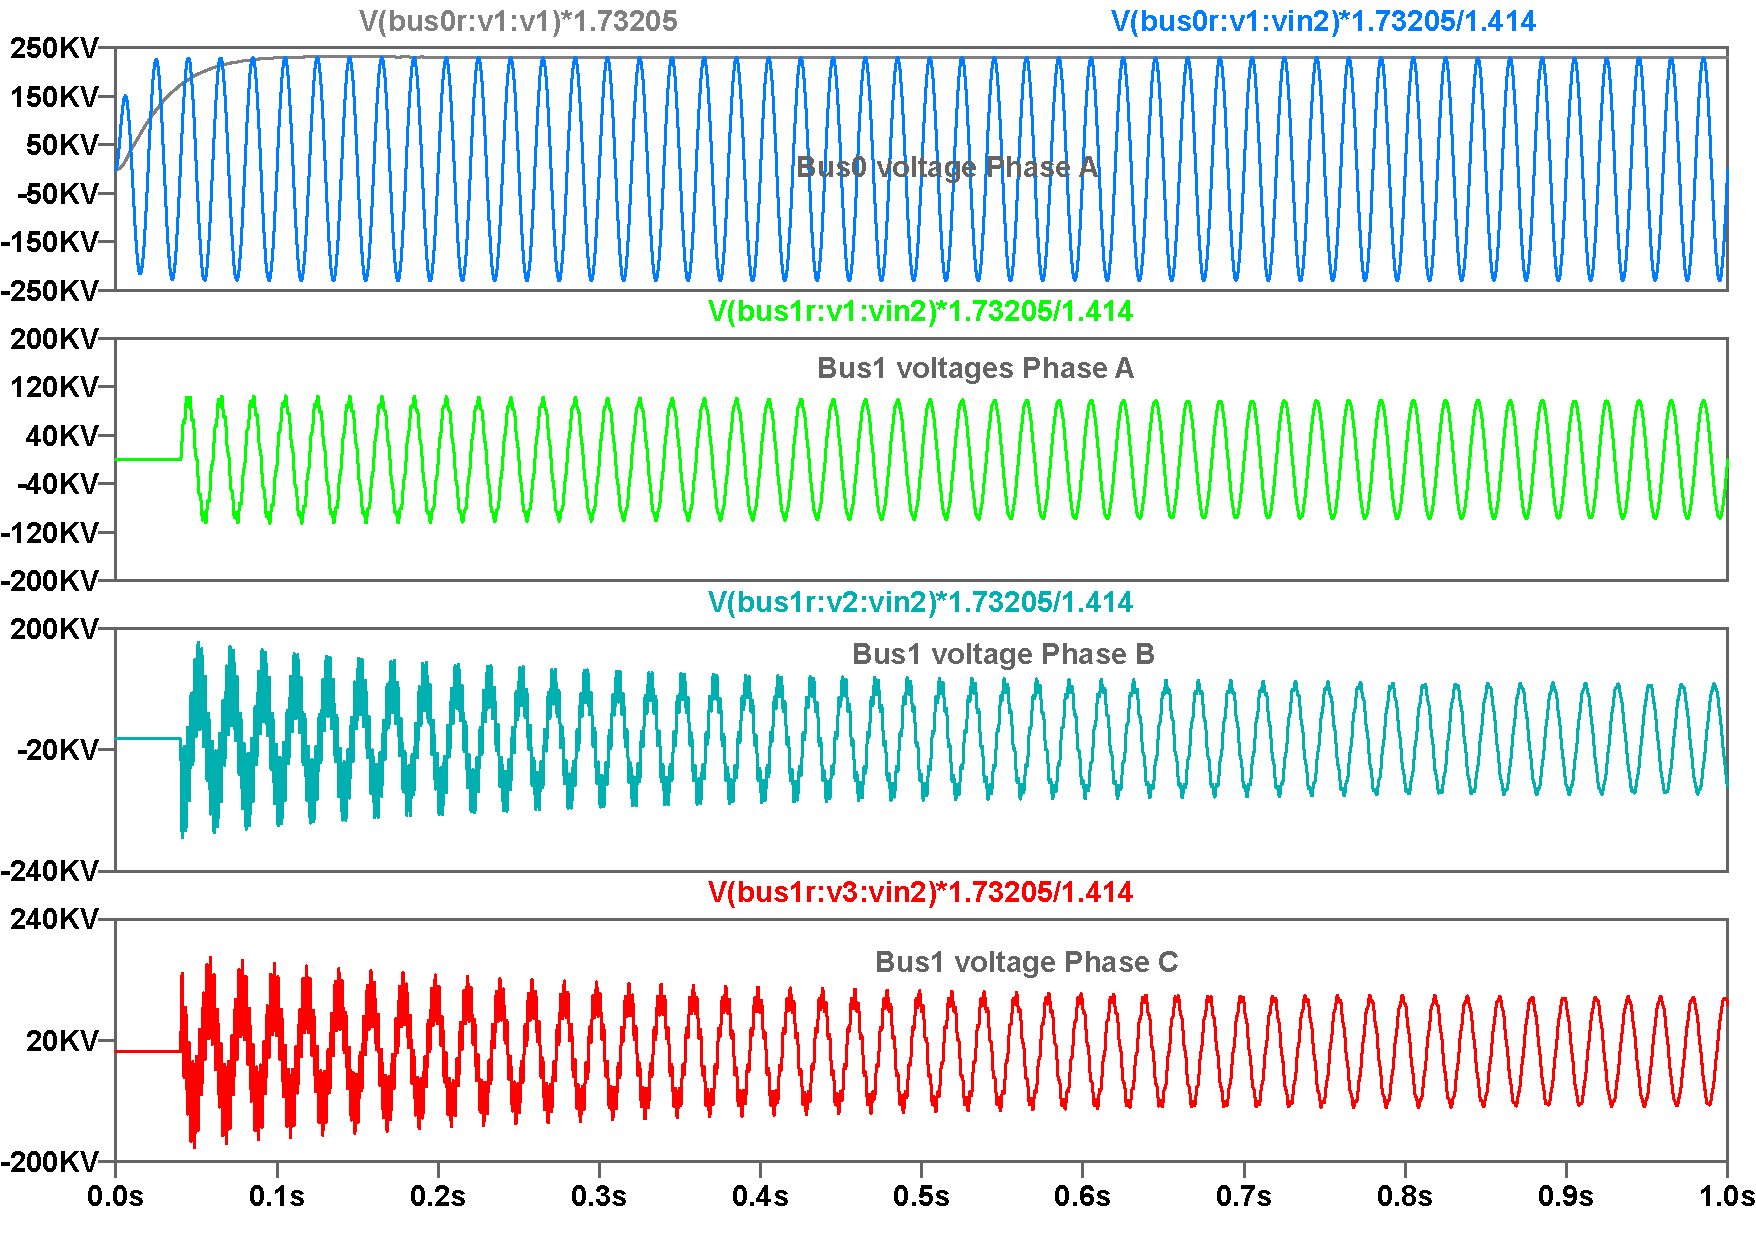
\includegraphics[width=0.90\textwidth]{figures/06_Switching_on_networks/Switching_on_networks_Bus0_Bus1_voltages-case4}
	\caption{Switching on networks voltages - case4}
	\label{fig:figure615}
\end{figure}

\begin{figure}[H]
	\centering
	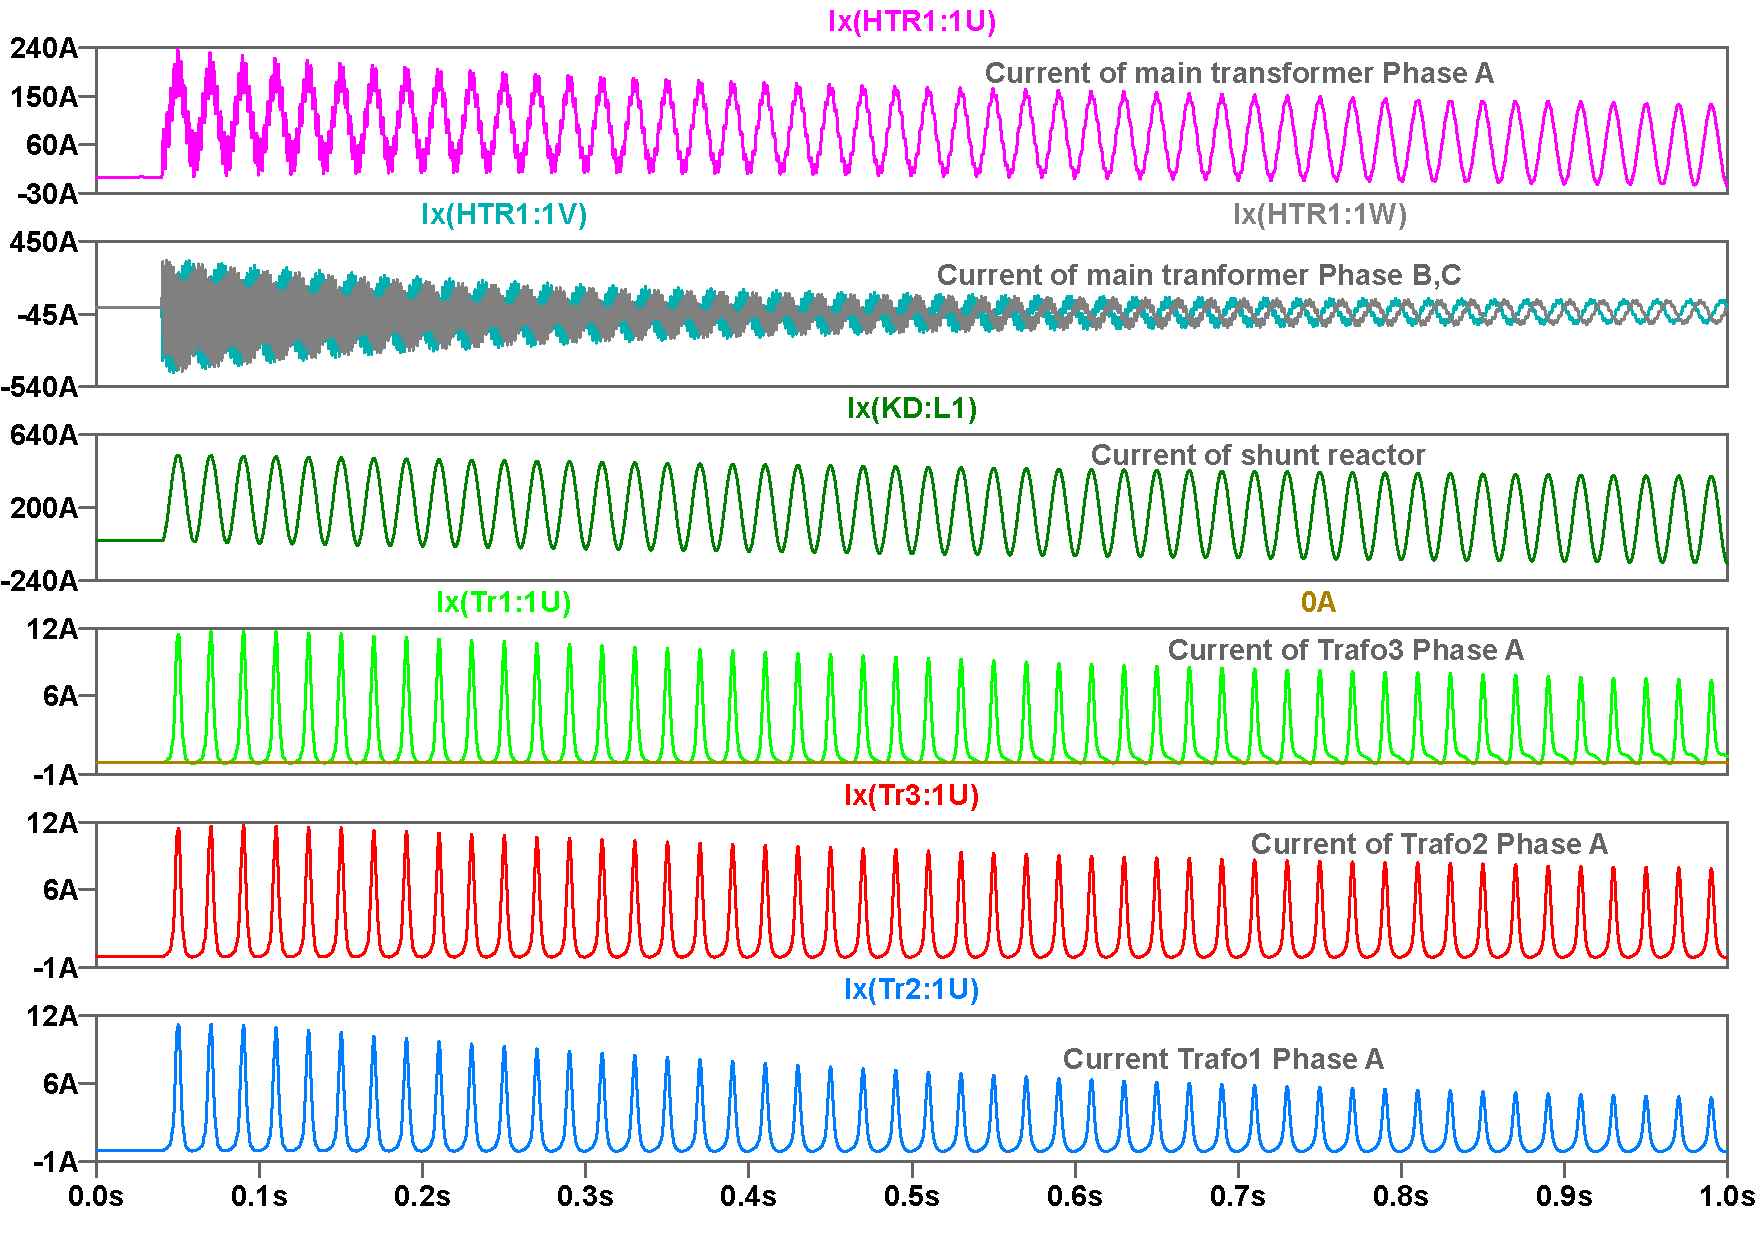
\includegraphics[width=0.90\textwidth]{figures/06_Switching_on_networks/Switching_on_networks_currents-case4}
	\caption{Switching on networks currents - case4}
	\label{fig:figure616}
\end{figure}

\begin{figure}[H]
	\centering
	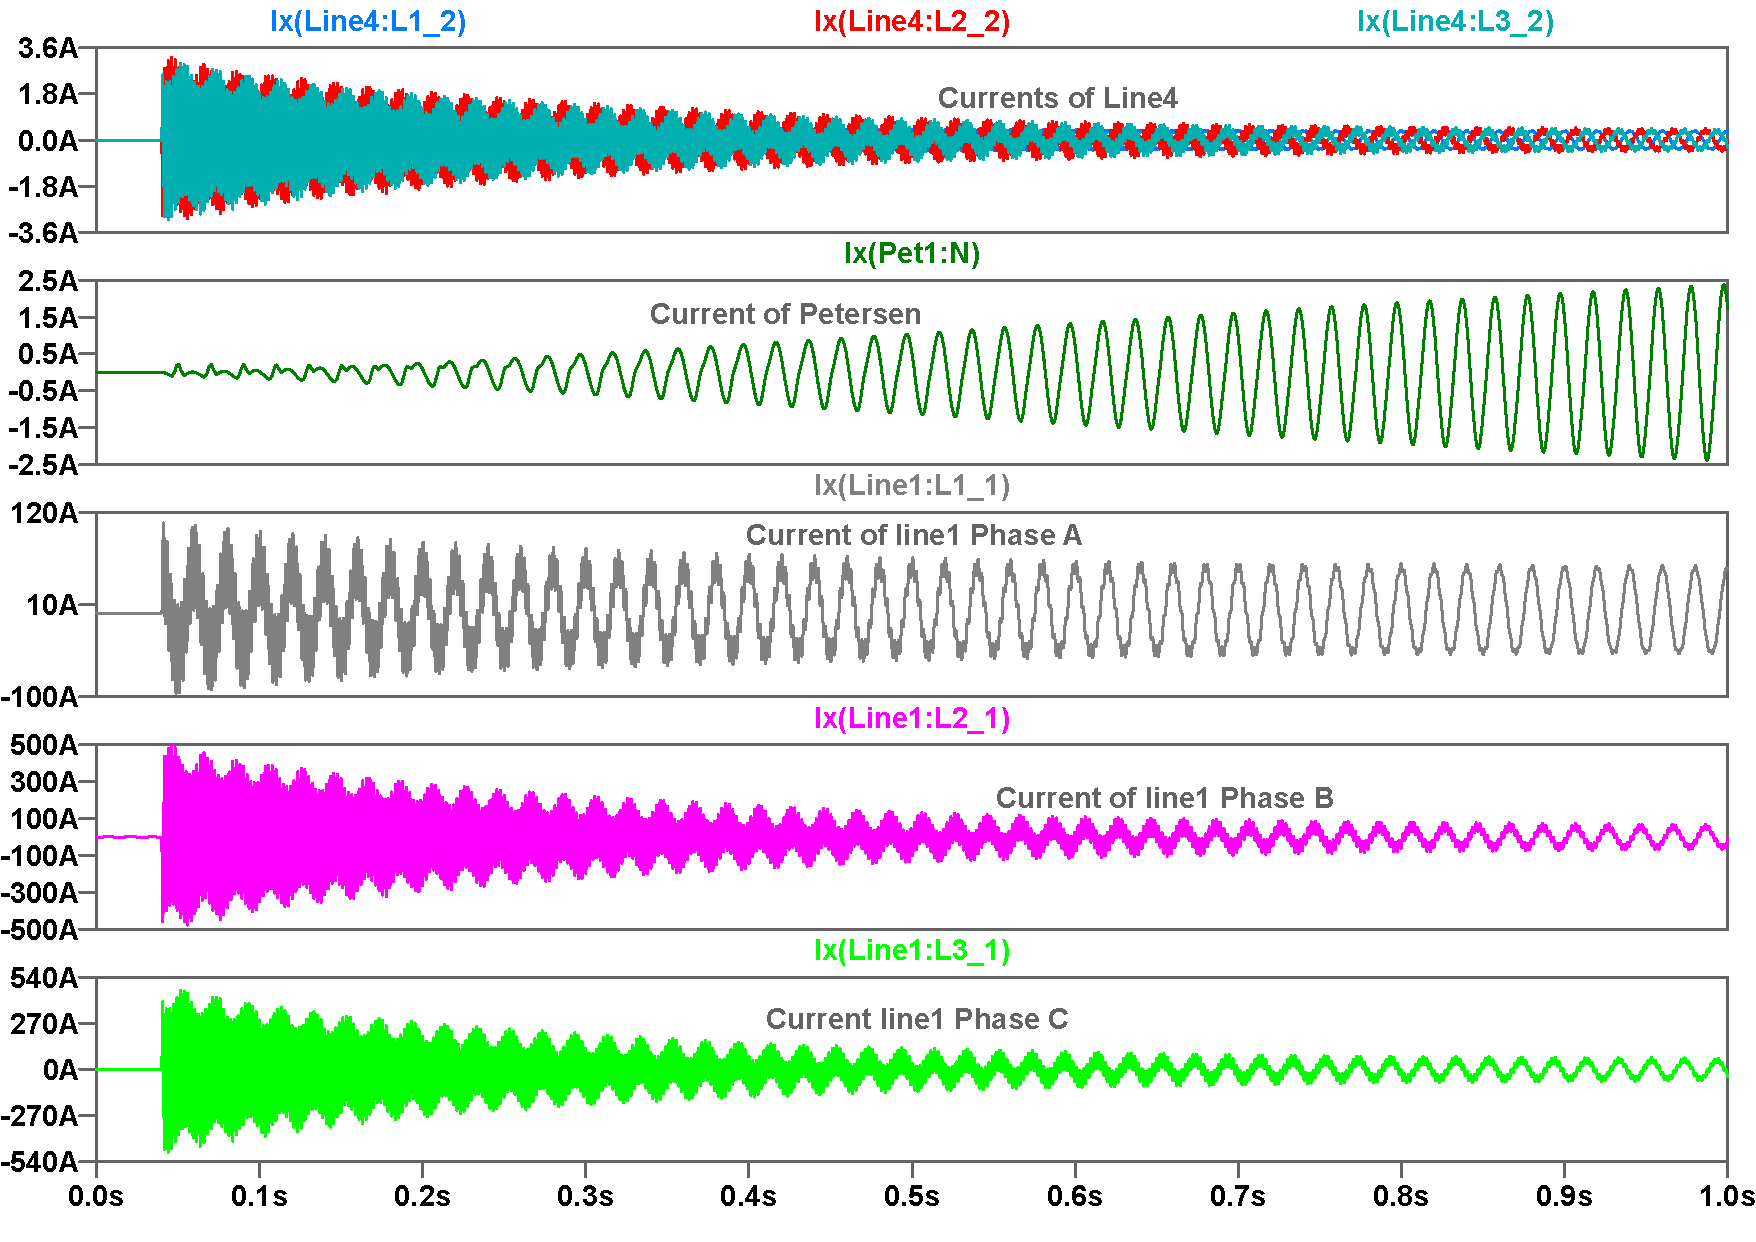
\includegraphics[width=0.90\textwidth]{figures/06_Switching_on_networks/Switching_on_networks_currents_Line1_Line4-case4}
	\caption{Switching on networks currents line1, line4 - case4}
	\label{fig:figure617}
\end{figure}

\begin{figure}[H]
	\centering
	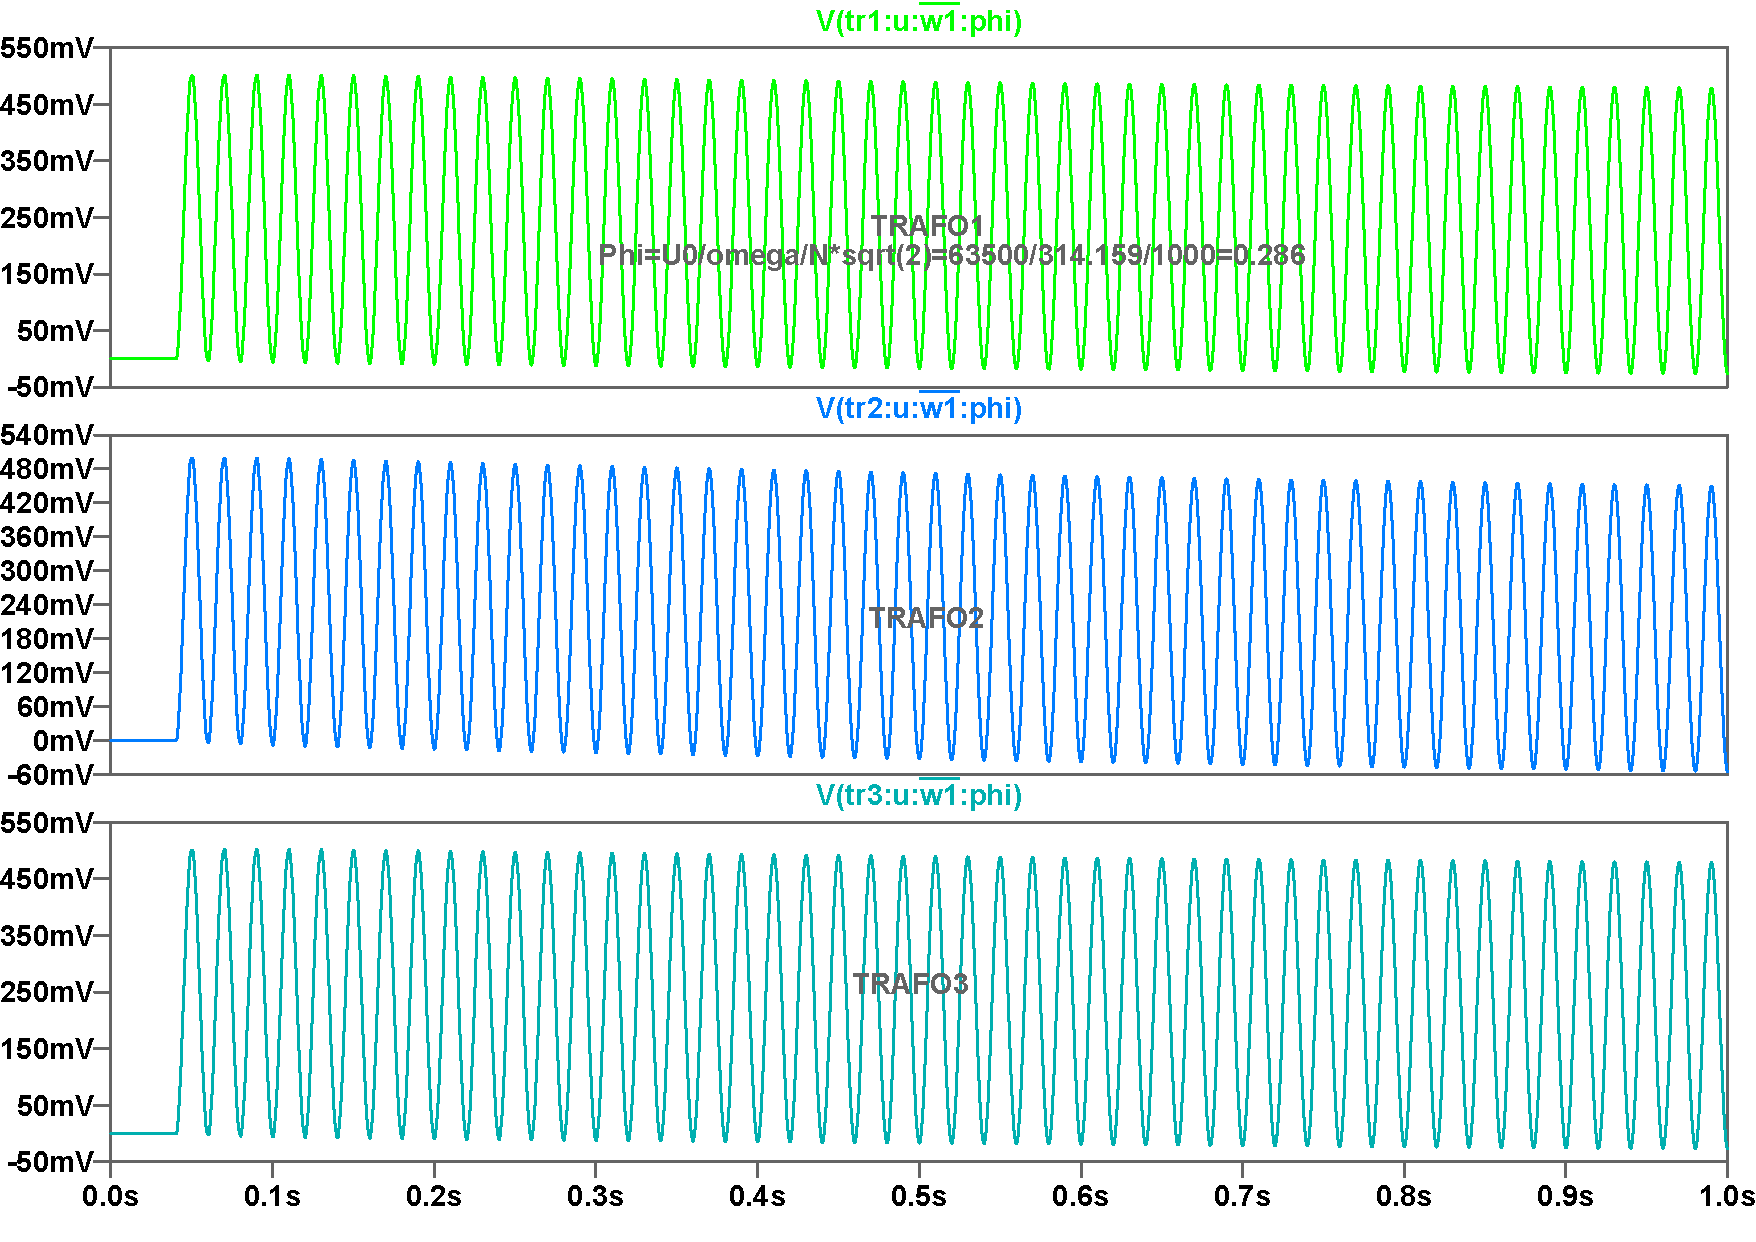
\includegraphics[width=0.90\textwidth]{figures/06_Switching_on_networks/Switching_on_networks_phi-case4}
	\caption{Switching on networks fluxes - case4}
	\label{fig:figure618}
\end{figure}

\begin{figure}[H]
	\centering
	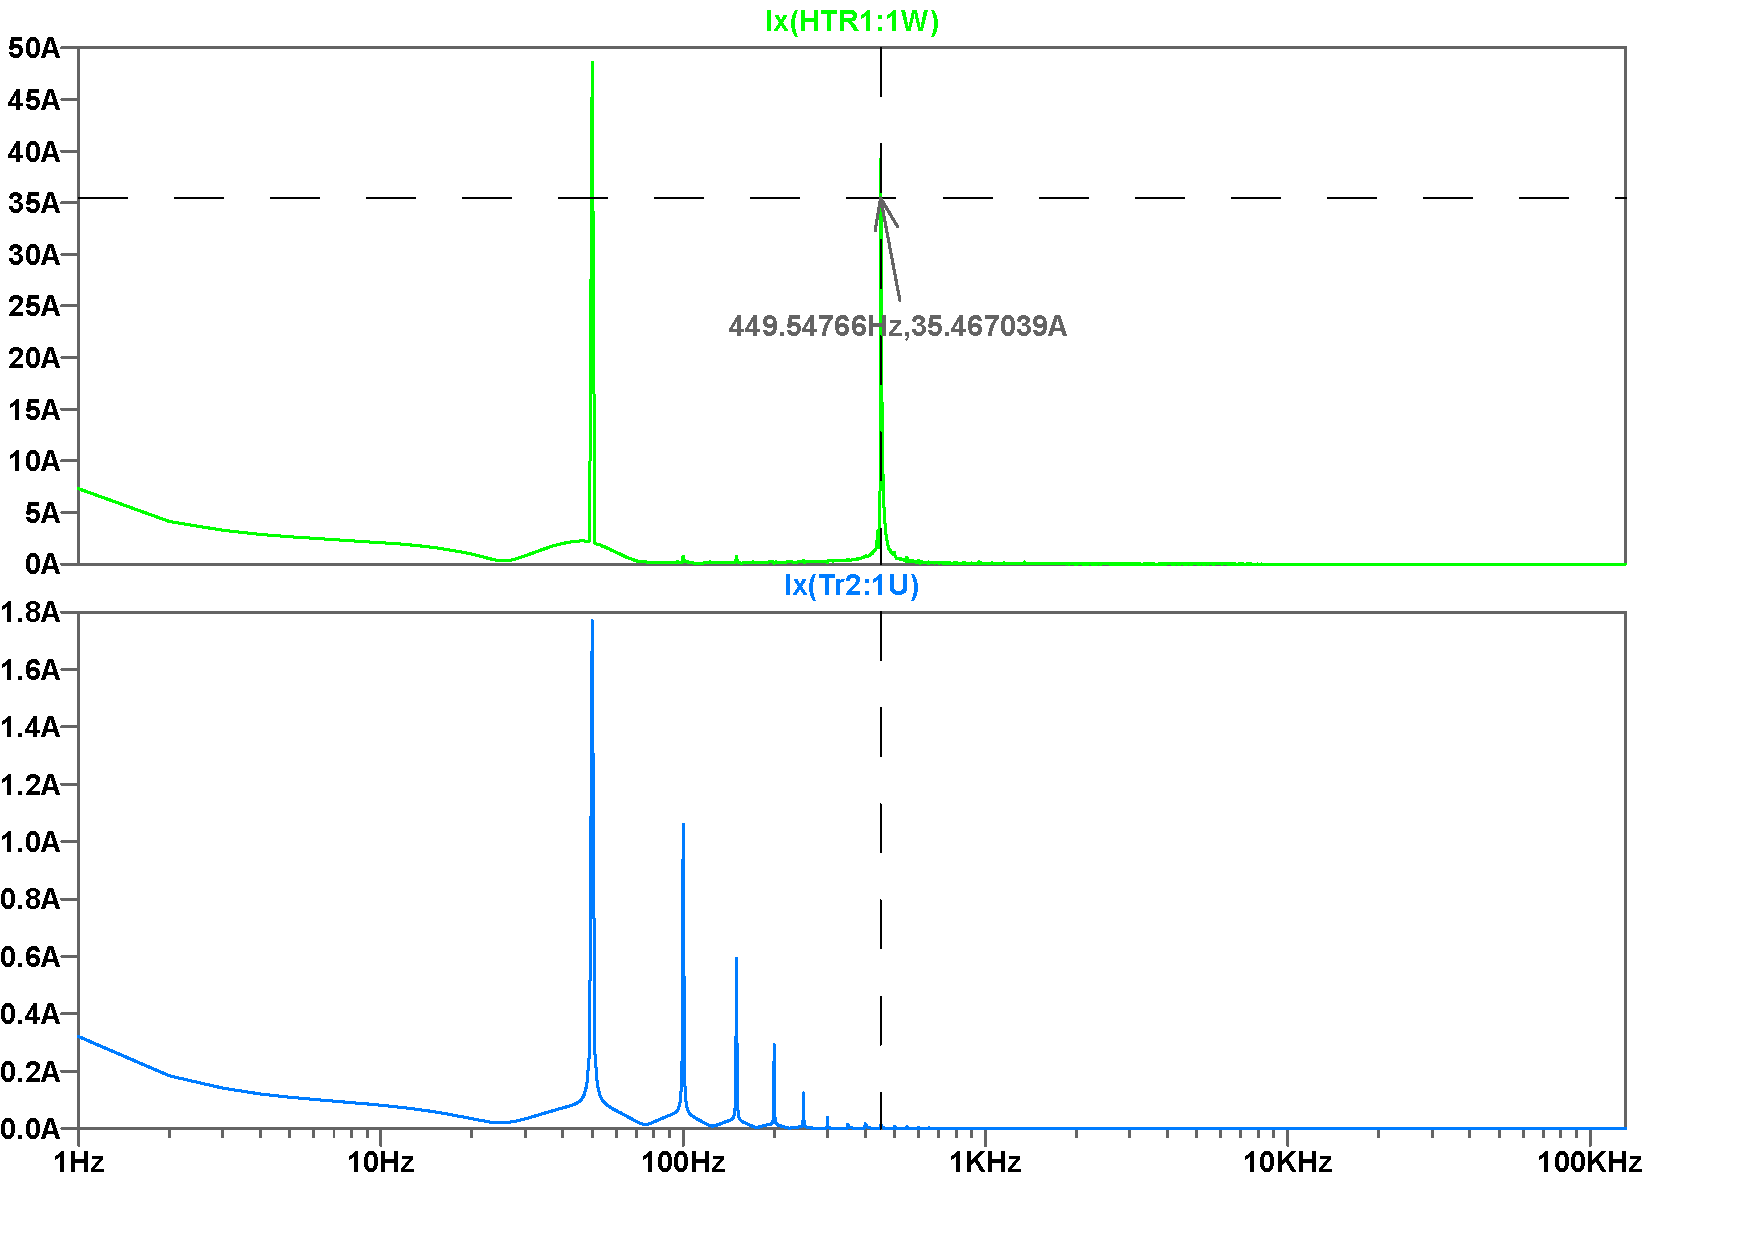
\includegraphics[width=0.90\textwidth]{figures/06_Switching_on_networks/Switching_on_networks_FFT_Transformer-case4}
	\caption{Switching on networks FFT - case4}
	\label{fig:figure619}
\end{figure}

% Measurement values table for the Power System Simulation book.
% Required packages are already loaded by the central preamble:
% booktabs, tabularx, array, siunitx, xcolor.

\begin{table}[htbp]
  \centering
  \caption{Signal ranges for Case 4. All values are peak values, bus values are multiplied by 1.73/1.414}
  \label{tab:measurement-values-case4}
  \small
  \setlength{\tabcolsep}{3.5pt}
  \renewcommand{\arraystretch}{1.18}
  \begin{tabularx}{\textwidth}{@{}
      >{\raggedright\arraybackslash}p{0.055\textwidth}
      >{\raggedright\arraybackslash}p{0.085\textwidth}
      >{\raggedright\arraybackslash}p{0.095\textwidth}
      >{\raggedright\arraybackslash}p{0.105\textwidth}
      >{\raggedright\arraybackslash}p{0.075\textwidth}
      >{\raggedright\arraybackslash}p{0.075\textwidth}
      Y@{}}
    \toprule
    \textbf{Meas.} &
    \textbf{Grid element} &
    \textbf{Phase} &
    \textbf{Voltage level} &
    \textbf{Min.} &
    \textbf{Max.} &
    \textbf{Notes} \\
    \midrule
    $V$ & Bus0  & Ph A       & \SI{220}{\kilo\volt} & \SI{-229}{\kilo\volt} & \SI{229}{\kilo\volt} & -- \\
    $V$ & Bus1  & Ph A,    & \SI{110}{\kilo\volt} & \SI{-100}{\kilo\volt} & \SI{100}{\kilo\volt} & -- \\
    $V$ & Bus1  & Ph B,C     & \SI{110}{\kilo\volt} & \SI{-180}{\kilo\volt} & \SI{180}{\kilo\volt} & -- \\
    $I$ & HTr1  & Ph A       & \SI{220}{\kilo\volt} & \SI{0}{\ampere} & \SI{230}{\ampere} & -- \\
    $I$ & HTr1  & Ph B, C    & \SI{220}{\kilo\volt} & \SI{-350}{\ampere} & \SI{300}{\ampere} & -- \\
    $I$ & KD1   & Ph A       & \SI{110}{\kilo\volt} & \SI{0}{\ampere} & \SI{520}{\ampere} & Steady state: \SI{300}{\ampere} \\
    $I$ & Tr1   & Ph A       & \SI{110}{\kilo\volt} & \SI{0}{\ampere} & \SI{11}{\ampere} & \\
    $I$ & Tr2   & Ph A       & \SI{110}{\kilo\volt} & \SI{0}{\ampere} & \SI{11}{\ampere} & Due to KD1: faster decrease of current \\
    $I$ & Tr3   & Ph A      & \SI{110}{\kilo\volt} & \SI{0}{\ampere} & \SI{11}{\ampere} & -- \\
    $I$ & Line4 & Ph A & \SI{110}{\kilo\volt} & \SI{-3}{\ampere} & \SI{3}{\ampere} & Small capacitive inrush current  \\
    $I$ & Line1 & Ph A & \SI{110}{\kilo\volt} & \SI{-100}{\ampere} & \SI{100}{\ampere} & High capacitive inrush current due to cable \\
    $I$ & Line1 & Ph B, C & \SI{110}{\kilo\volt} & \SI{-500}{\ampere} & \SI{500}{\ampere} & High capacitive inrush current due to cable \\
    $I$ & Pet1 & Ph N & \SI{110}{\kilo\volt} & \SI{-2.5}{\ampere} & \SI{2.5}{\ampere} & Longtime value very small \\
    $V$ & Pet1 & Ph N & \SI{110}{\kilo\volt} & \SI{-600}{\volt} & \SI{600}{\volt} & Longtime value very small \\
    $\Phi$ & Tr1 & Ph A, B, C   & \SI{110}{\kilo\volt} & \SI{0}{\weber} & \SI{0.5}{\weber} & Nominal flux: 
    \SI{0.288}{\weber} \\
    FFT & HTr1  & Ph C       & \SI{220}{\kilo\volt} & \SI{50}{\hertz} & \SI{450}{\hertz} & Only \SI{50}{\hertz} and \SI{450}{\hertz} \\
    FFT & Tr2   & Ph A       & \SI{110}{\kilo\volt} & \SI{50}{\hertz} & \SI{250}{\hertz} & \SI{50}{\hertz}, \SI{100}{\hertz}, \SI{150}{\hertz}, \SI{200}{\hertz}, and \SI{250}{\hertz} \\
    \bottomrule
  \end{tabularx}
\end{table}


\section{Case 5: Energizing a Larger Network}
\label{sec:network-larger-capacitance}

Set \texttt{cf=5} to multiply the cable-network capacitance by five. The
capacitive currents are approximately twice, rather than five times, those of
\cref{sec:network-closing-voltage-zero}. The larger capacitance lowers the
dominant resonance from approximately \SI{400}{\hertz} to
approximately \SI{180}{\hertz}. 


As can be seen from the low bias voltage and the low Petersen-coil current, the Petersen circuit is not yet optimally tuned. If we look at the AC analysis, we can see that the resonance point is at approximately \SI{45}{\hertz}. You can see this by determining the beat frequency in the transient analysis. So the Petersen circuit’s tuning still needs to be adjusted (see Switching\_Networks\_AC.asc). NOTE: At \SI{1250}{\ampere}, the Petersen current is, of course, much too high and would place too heavy a load on the transformer. The transformer current of Transformer 1 starts at approximately \SI{50}{\ampere} and then fluctuates up and down. This is due to the voltage containing 180Hz+50Hz components, which also fluctuates up and down at the beginning and, consequently, the integral of the voltage which gives the flux. The voltage of the \SI{110}{\kilo\volt} Phase A starts at \SI{120}{\kilo\volt}, while the voltage of the other phases initially reaches between \SI{180}{\kilo\volt} and \SI{200}{\kilo\volt}. The current through the main transformer in Phase A is approximately \SI{530}{\ampere} to \SI{-160}{\ampere}, while the current in Phases B and C is approximately \SI{1}{\kilo\ampere}. These currents are primarily caused by capacitive inrush currents and are due to the now larger capacitive network. The current through the KD ranges from \SI{0}{\ampere} to \SI{620}{\ampere} and decreases rapidly. The current in Line 1 is approximately \SI{600}{\ampere} in Phase A and approximately \SI{1.3}{\kilo\ampere} in the other two phases, which is much higher than in Case 1.  The current in Line 4 is very low, at \SI{1}{\ampere} to \SI{2}{\ampere}, since the charging current of an overhead line is very small. The FFT of the current in phase C on the primary side of the main transformer shows a peak at approximately \SI{180}{\hertz}, as shown in the associated calculation. Here, the \SI{180}{\hertz} component is even higher than the \SI{50}{\hertz} component. 
The maximum flux of the medium-voltage transformers is initially about \SI{600}{\milli\weber}, which is slightly higher than in Case 1.
 


For calculation of the dominant frequency of the circuit like in calculation \ref{calc:whole-network-resonance}
the inductances specified on the \SI{220}{\kilo\volt} side must be referred to
the \SI{110}{\kilo\volt} side. With a voltage ratio of 2, impedance and
inductance are divided by $2^2=4$ when referred from the
\SI{220}{\kilo\volt} side to the \SI{110}{\kilo\volt} side. 
The source and transformer inductances are $L_{\mathrm{net}}=\SI{0.0077}{\henry}$ and $L_{\mathrm{Tr}}=\SI{0.154}{\henry}$. The sum of capacitance is now 5*4000nF=20000nF. \\
We obtained from the file \texttt{Trafo\_YY0\_220k\_110k\_200MVA\_Daten.asc} 
the data for the transformer.

\begin{calculation}{Dominant cable-network resonance}{whole-network-resonance3}
	\begin{align}
		L_{\mathrm{eq}}&=\frac{L_{\mathrm{net}}}{4}
		+\frac{L_{\mathrm{Tr}}}{4}
		=\frac{\SI{0.0077}{\henry}+\SI{0.154}{\henry}}{4}
		=\SI{0.04}{\henry},\\
		C&=\SI{20000}{\nano\farad},\\
		f_{\mathrm r}&=\frac{1}{2\pi\sqrt{L_{\mathrm{eq}}C}}
		\approx\boxed{\SI{178}{\hertz}}.
	\end{align}
\end{calculation}

\begin{figure}[H]
	\centering
	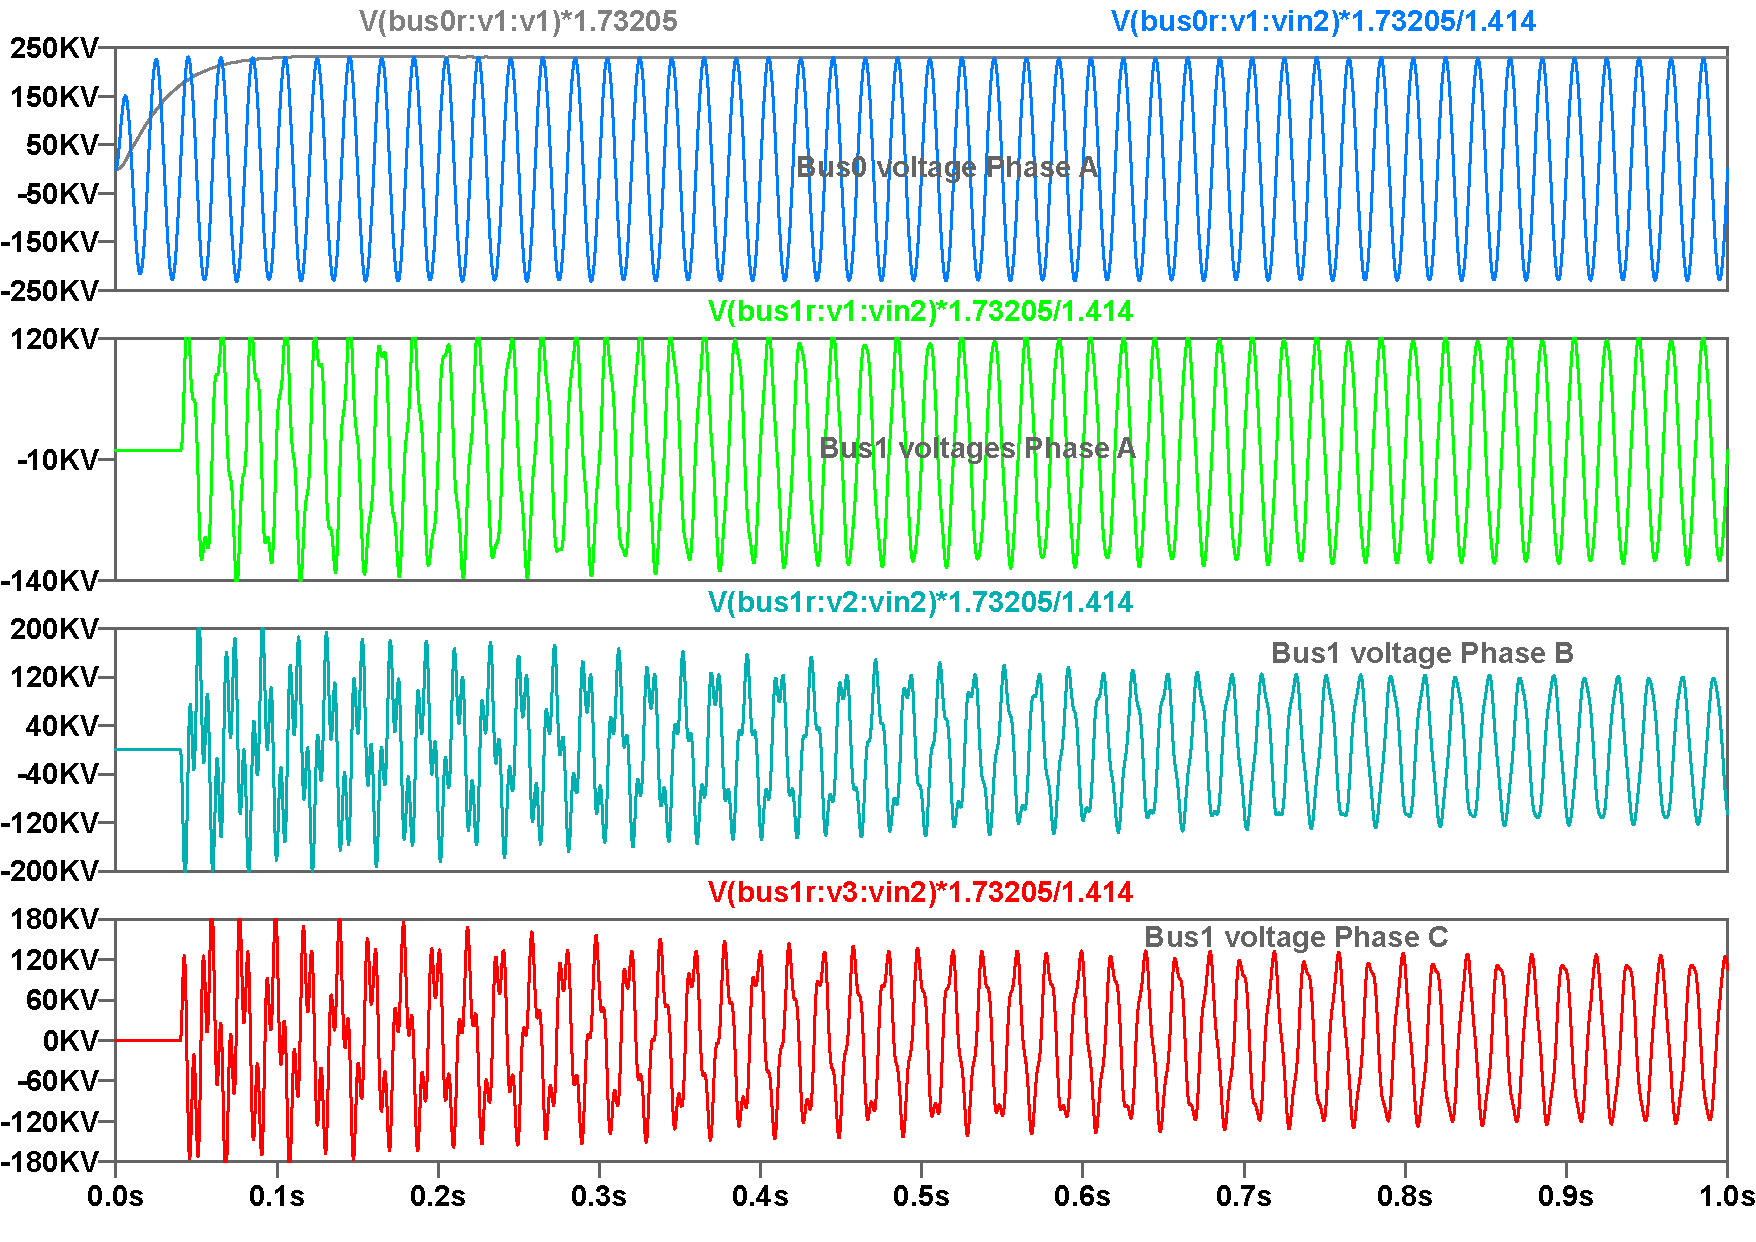
\includegraphics[width=0.90\textwidth]{figures/06_Switching_on_networks/Switching_on_networks_Bus0_Bus1_voltages-case5}
	\caption{Switching on networks voltages - case5}
	\label{fig:figure620}
\end{figure}

\begin{figure}[H]
	\centering
	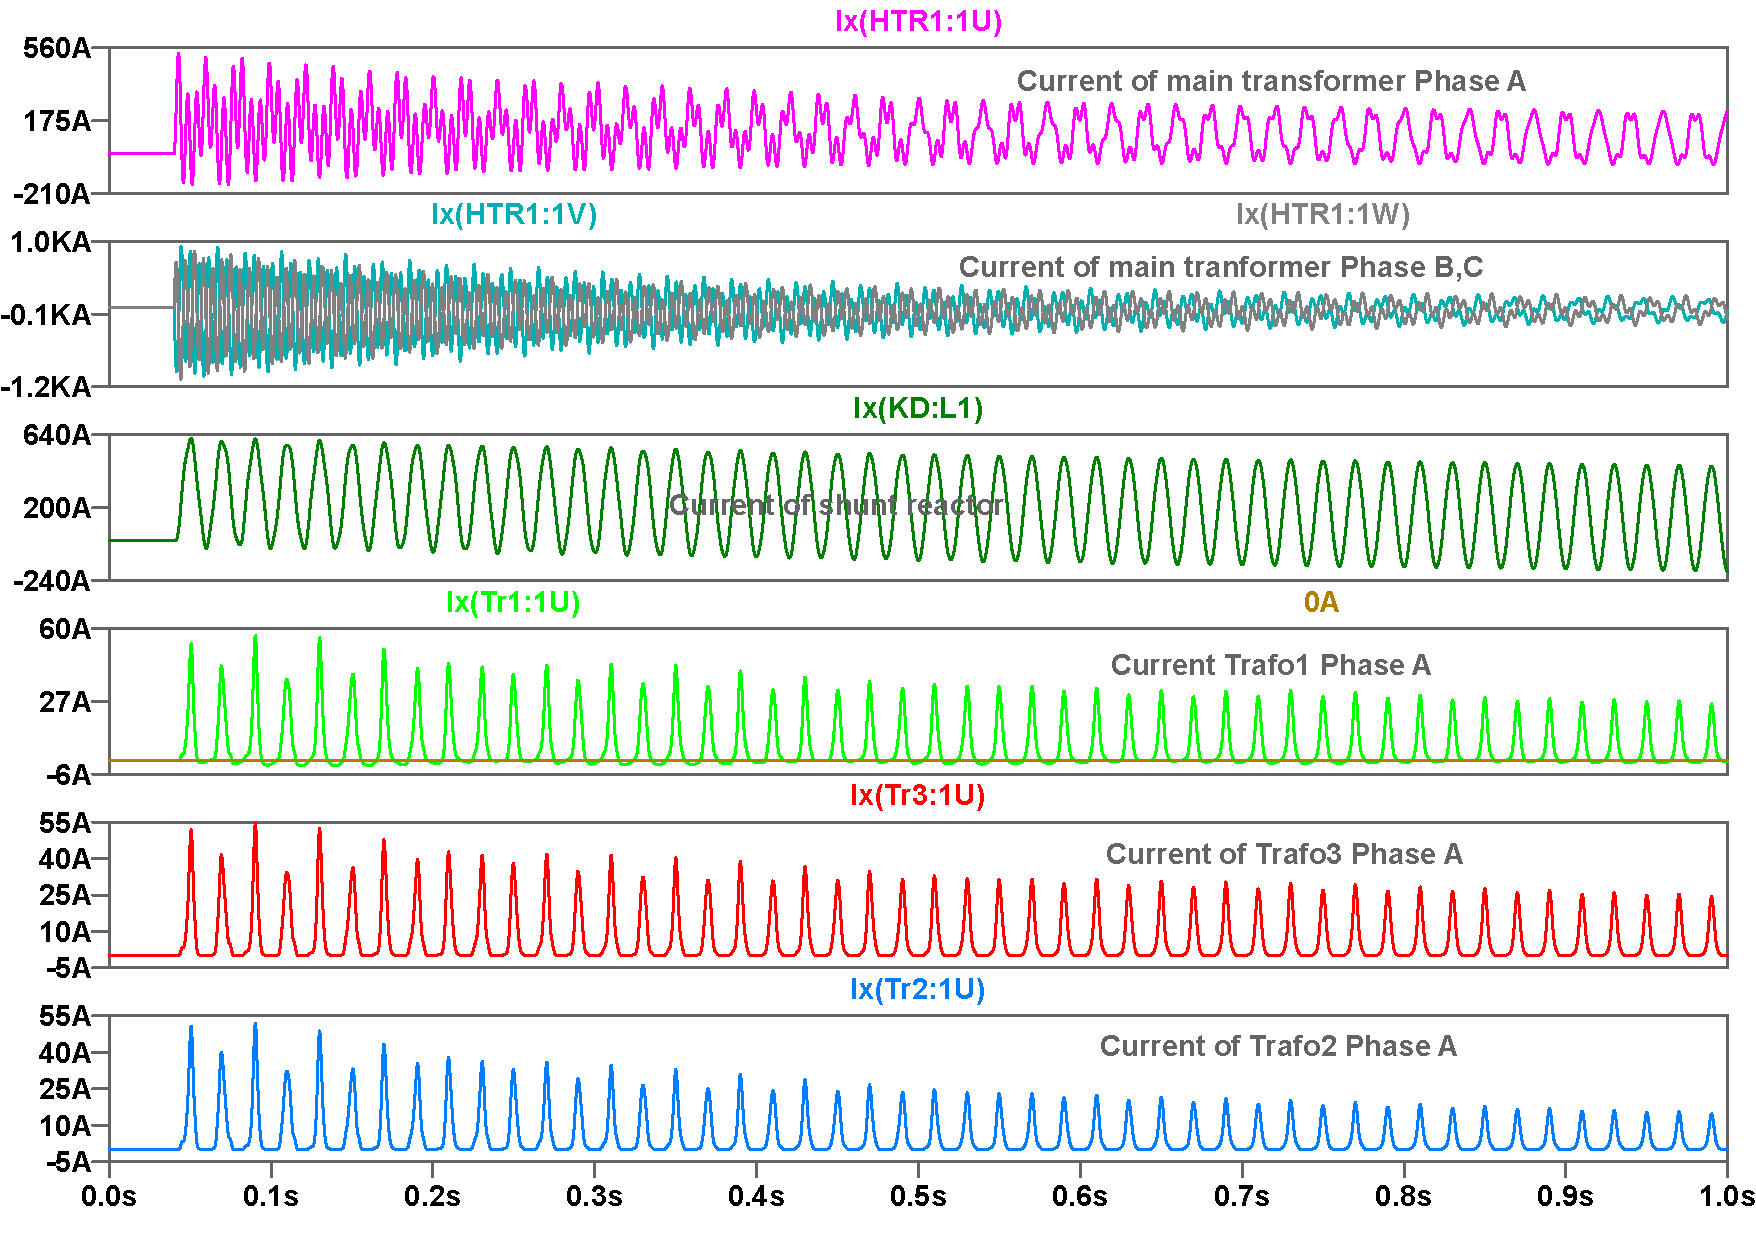
\includegraphics[width=0.90\textwidth]{figures/06_Switching_on_networks/Switching_on_networks_currents-case5}
	\caption{Switching on networks currents - case5}
	\label{fig:figure621}
\end{figure}

\begin{figure}[H]
	\centering
	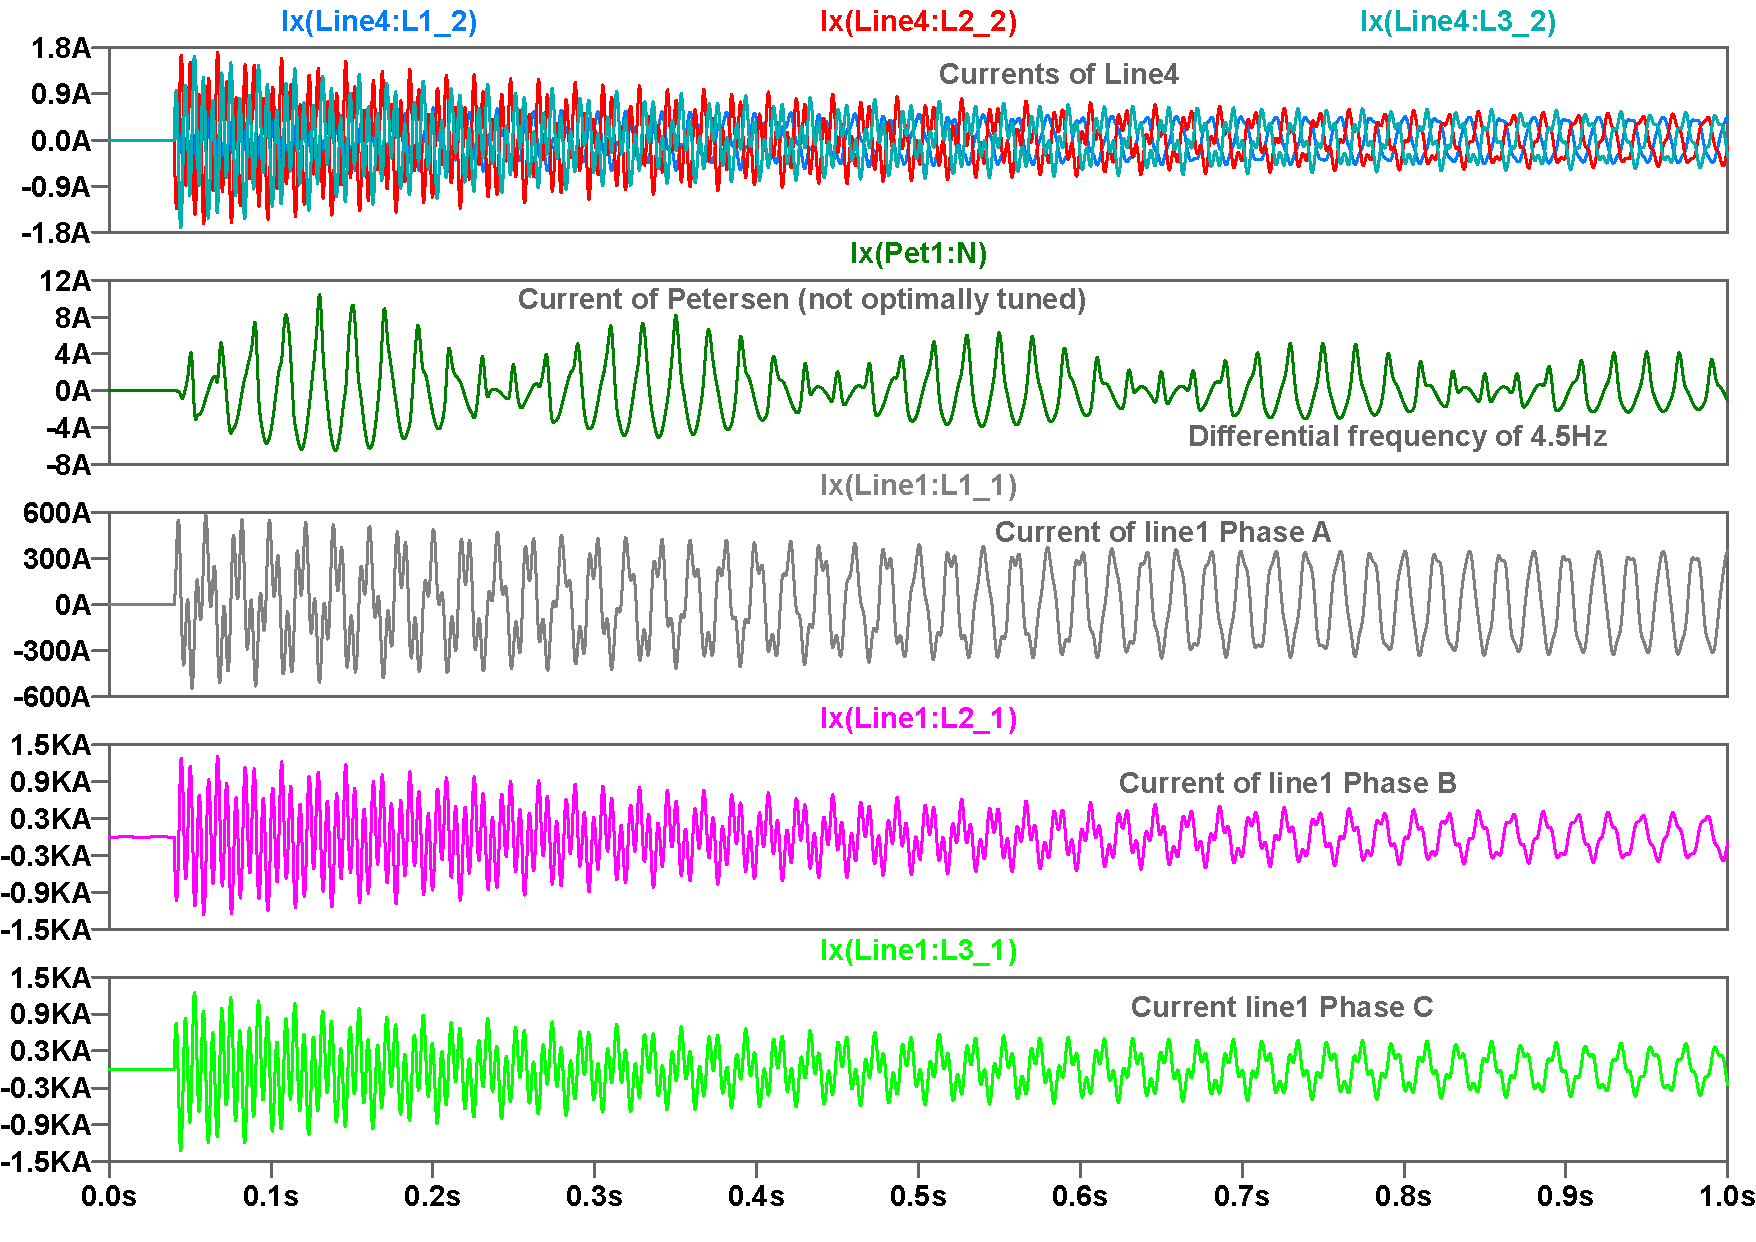
\includegraphics[width=0.90\textwidth]{figures/06_Switching_on_networks/Switching_on_networks_currents_Line1_Line4-case5}
	\caption{Switching on networks currents line1, line4 - case5}
	\label{fig:figure622}
\end{figure}

\begin{figure}[H]
	\centering
	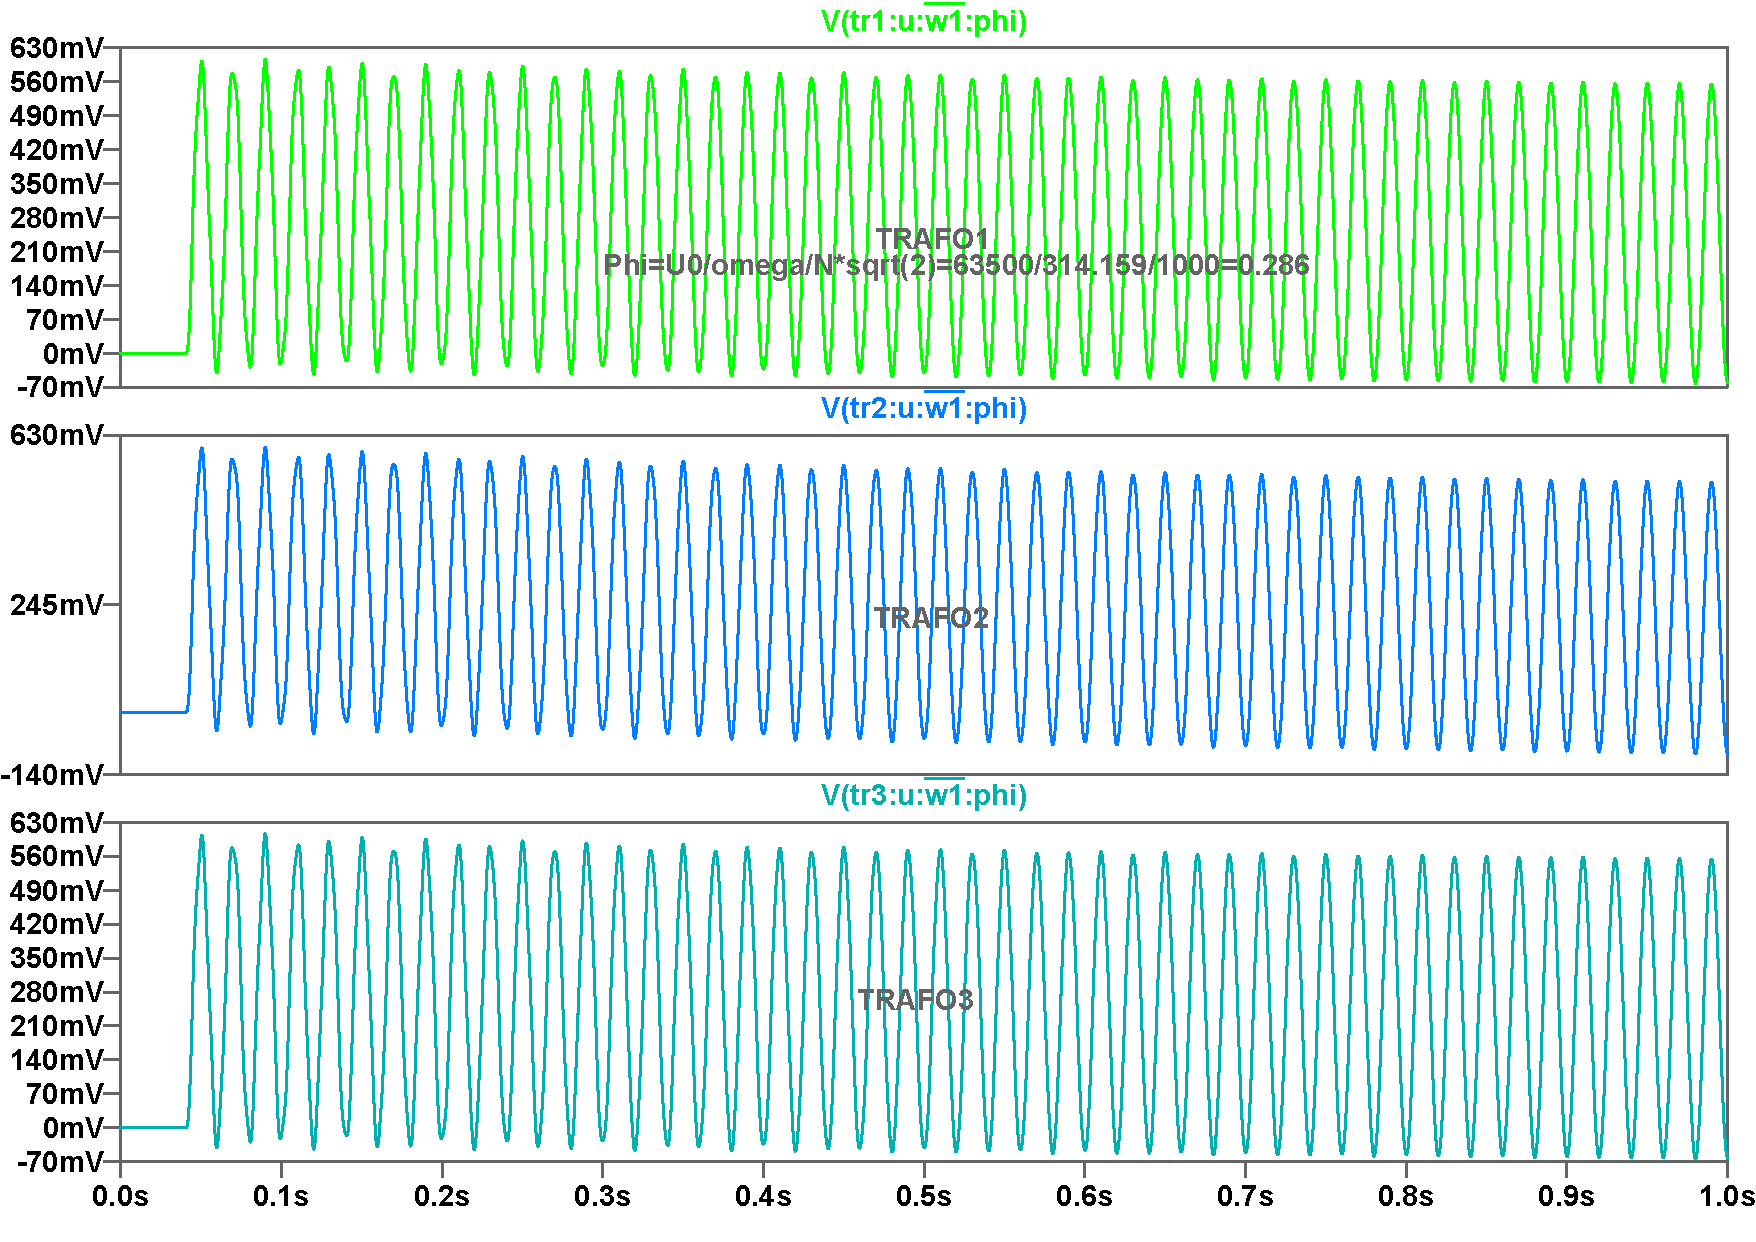
\includegraphics[width=0.90\textwidth]{figures/06_Switching_on_networks/Switching_on_networks_phi-case5}
	\caption{Switching on networks fluxes - case5}
	\label{fig:figure623}
\end{figure}

\begin{figure}[H]
	\centering
	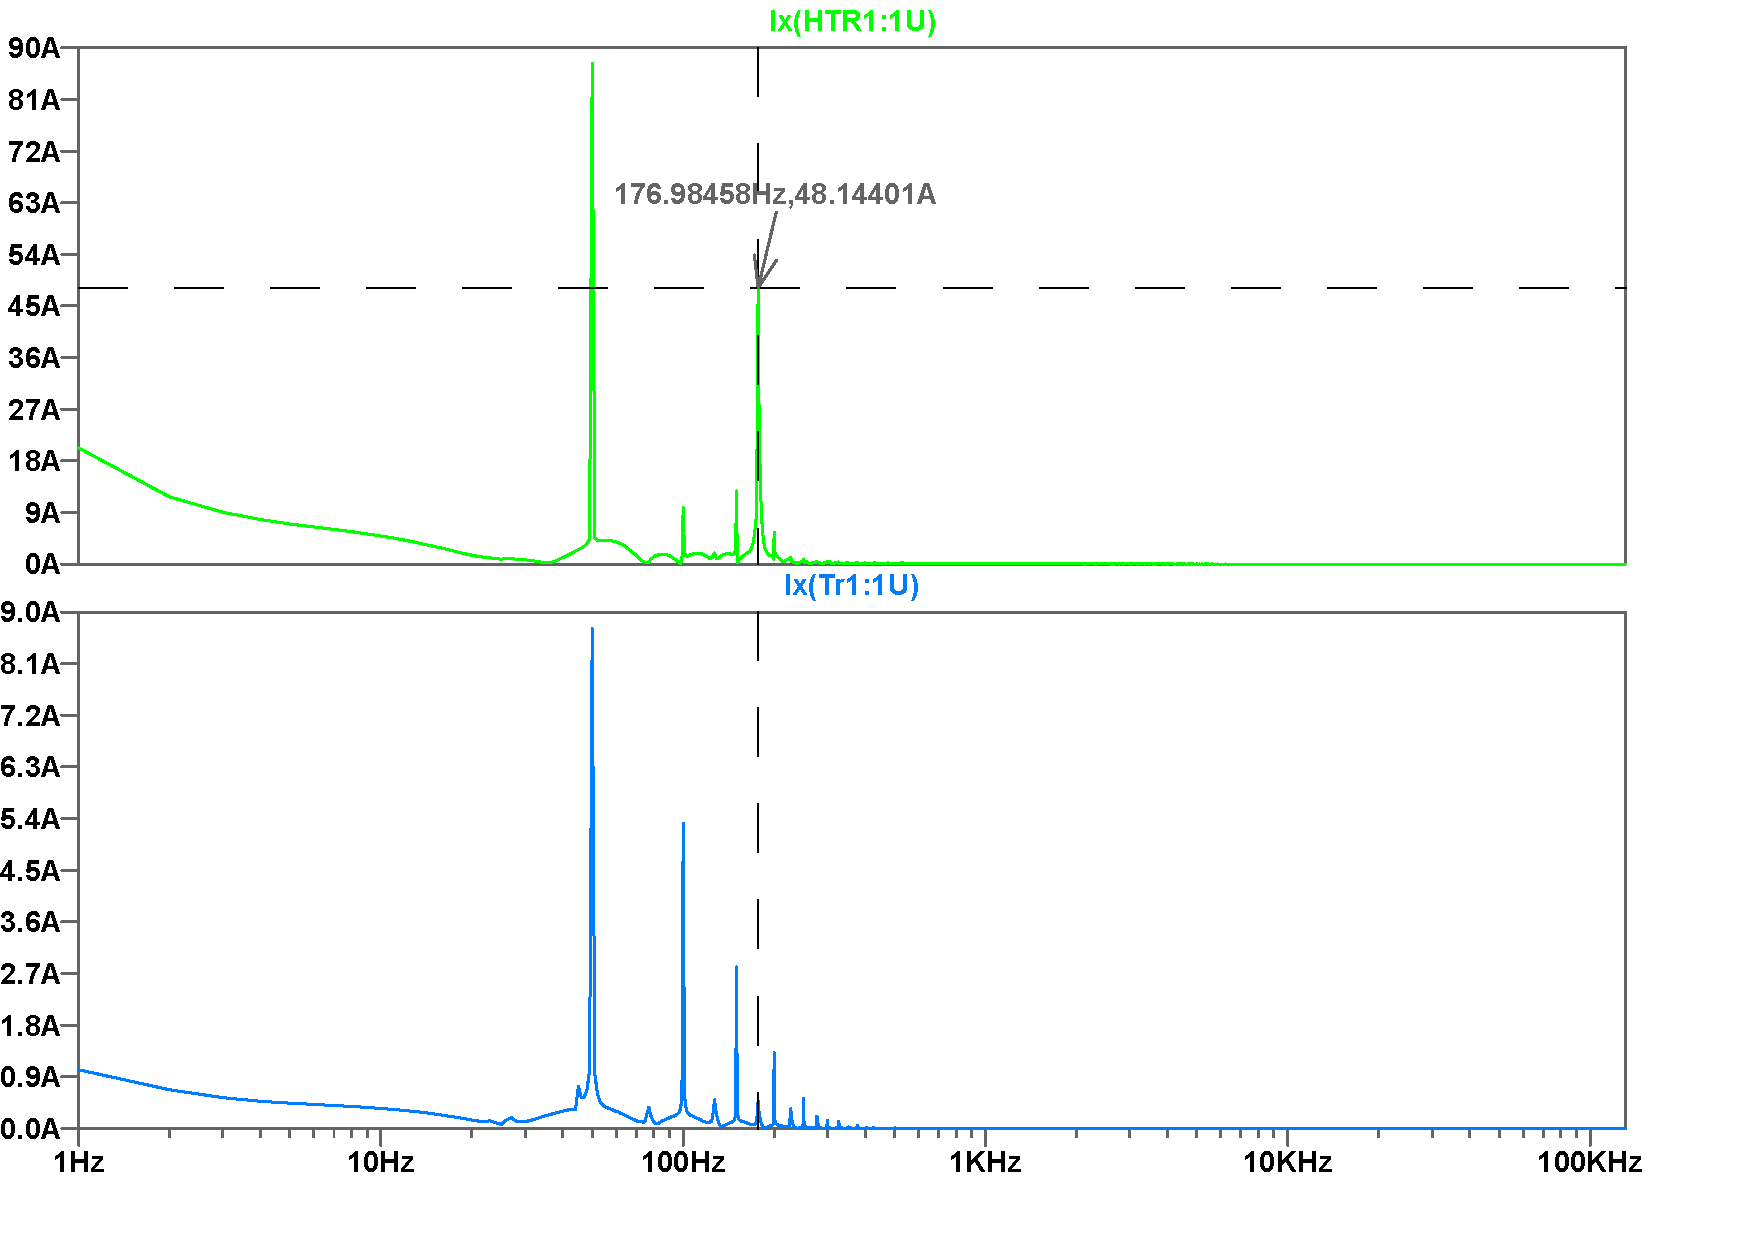
\includegraphics[width=0.90\textwidth]{figures/06_Switching_on_networks/Switching_on_networks_FFT_Transformer-case5}
	\caption{Switching on networks FFT - case5}
	\label{fig:figure624}
\end{figure}


% Measurement values table for the Power System Simulation book.
% Required packages are already loaded by the central preamble:
% booktabs, tabularx, array, siunitx, xcolor.

\begin{table}[htbp]
  \centering
  \caption{Signal ranges for Case 5. All values are peak values, bus values are multiplied by 1.73/1.414}
  \label{tab:measurement-values-case5}
  \small
  \setlength{\tabcolsep}{3.5pt}
  \renewcommand{\arraystretch}{1.18}
  \begin{tabularx}{\textwidth}{@{}
      >{\raggedright\arraybackslash}p{0.055\textwidth}
      >{\raggedright\arraybackslash}p{0.085\textwidth}
      >{\raggedright\arraybackslash}p{0.095\textwidth}
      >{\raggedright\arraybackslash}p{0.105\textwidth}
      >{\raggedright\arraybackslash}p{0.075\textwidth}
      >{\raggedright\arraybackslash}p{0.075\textwidth}
      Y@{}}
    \toprule
    \textbf{Meas.} &
    \textbf{Grid element} &
    \textbf{Phase} &
    \textbf{Voltage level} &
    \textbf{Min.} &
    \textbf{Max.} &
    \textbf{Notes} \\
    \midrule
    $V$ & Bus0  & Ph A       & \SI{220}{\kilo\volt} & \SI{-229}{\kilo\volt} & \SI{229}{\kilo\volt} & -- \\
    $V$ & Bus1  & Ph A,    & \SI{110}{\kilo\volt} & \SI{-140}{\kilo\volt} & \SI{120}{\kilo\volt} & -- \\
    $V$ & Bus1  & Ph B,C     & \SI{110}{\kilo\volt} & \SI{-180}{\kilo\volt} & \SI{180}{\kilo\volt} & -- \\
    $I$ & HTr1  & Ph A       & \SI{220}{\kilo\volt} & \SI{-160}{\ampere} & \SI{530}{\ampere} & -- \\
    $I$ & HTr1  & Ph B, C    & \SI{220}{\kilo\volt} & \SI{-1}{\kilo\ampere} & \SI{1}{\kilo\ampere} & -- \\
    $I$ & KD1   & Ph A       & \SI{110}{\kilo\volt} & \SI{0}{\ampere} & \SI{620}{\ampere} & Steady state: \SI{300}{\ampere} \\
    $I$ & Tr1   & Ph A       & \SI{110}{\kilo\volt} & \SI{0}{\ampere} & \SI{54}{\ampere} &  Fluctuating \\
    $I$ & Tr2   & Ph A       & \SI{110}{\kilo\volt} & \SI{0}{\ampere} & \SI{52}{\ampere} &  Fluctuating \\
    $I$ & Tr3   & Ph A      & \SI{110}{\kilo\volt} & \SI{0}{\ampere} & \SI{52}{\ampere} &  Fluctuating \\
    $I$ & Line4 & Ph A & \SI{110}{\kilo\volt} & \SI{-1.6}{\ampere} & \SI{1.6}{\ampere} & Small capacitive inrush current  \\
    $I$ & Line1 & Ph A & \SI{110}{\kilo\volt} & \SI{-530}{\ampere} & \SI{600}{\ampere} & High capacitive inrush current due to cable \\
    $I$ & Line1 & Ph B, C & \SI{110}{\kilo\volt} & \SI{-1.3}{\kilo\ampere} & \SI{1.3}{\kilo\ampere} & High capacitive inrush current due to cable \\
    $I$ & Pet1 & Ph N & \SI{110}{\kilo\volt} & \SI{-6}{\ampere} & \SI{10}{\ampere} & Fluctuating, Longtime value very small \\
    $V$ & Pet1 & Ph N & \SI{110}{\kilo\volt} & \SI{-800}{\volt} & \SI{600}{\volt} & Fluctuating, Longtime value very small \\
    $\Phi$ & Tr1 & Ph A, B, C   & \SI{110}{\kilo\volt} & \SI{0}{\weber} & \SI{0.60}{\weber} & Nominal flux: 
    \SI{0.288}{\weber} \\
    FFT & HTr1  & Ph C       & \SI{220}{\kilo\volt} & \SI{50}{\hertz} & \SI{178}{\hertz} & mostly \SI{50}{\hertz} and \SI{178}{\hertz} \\
    FFT & Tr2   & Ph A       & \SI{110}{\kilo\volt} & \SI{50}{\hertz} & \SI{250}{\hertz} & \SI{50}{\hertz}, \SI{100}{\hertz}, \SI{150}{\hertz}, \SI{200}{\hertz}, and \SI{250}{\hertz} \\
    \bottomrule
  \end{tabularx}
\end{table}




\section{Case 6: Energization with Load}
\label{sec:network-energization-with-load}

Set \texttt{lf=0.5}. The connected load strongly dampens the overvoltages caused
by the high-frequency capacitive charging currents, and these oscillations
decay rapidly. Transformer inrush currents remain present because they are caused
by the transient core flux. Among the direct-switching cases considered so
far, this case produces the smallest overvoltages.

The current on the 10.6 kV side of the load is 360 A,
which is approximately 36 A on the 110 kV side. The currents on the 110 kV side are
a mixture of inrush currents and load currents.
It is often claimed in the literature that the load current
reduces the inrush of the magnetizing current.
This is not really the case. This can be easily demonstrated by simultaneously simulating three identical transformers:
a) Set m=1 for Transformer 1 and apply a load to it. This measures the load current on the primary side.
b) Set m = 9 for Transformer 2 and set the load to zero.
c) For Transformer 3, set m=9 and connect the same load. The resulting currents can then be compared.
Now you can see that when adding the primary currents I(Transformer 1) + I(Transformer 2), the resulting current is approximately equal to I(Transformer 3). Any reduction in inrush current is very small in this example. The transformer inrush is simply “hidden” in the total current but is always present. See ltspice file \texttt{Hidden\_inrush.asc}
 
\begin{figure}[H]
	\centering
	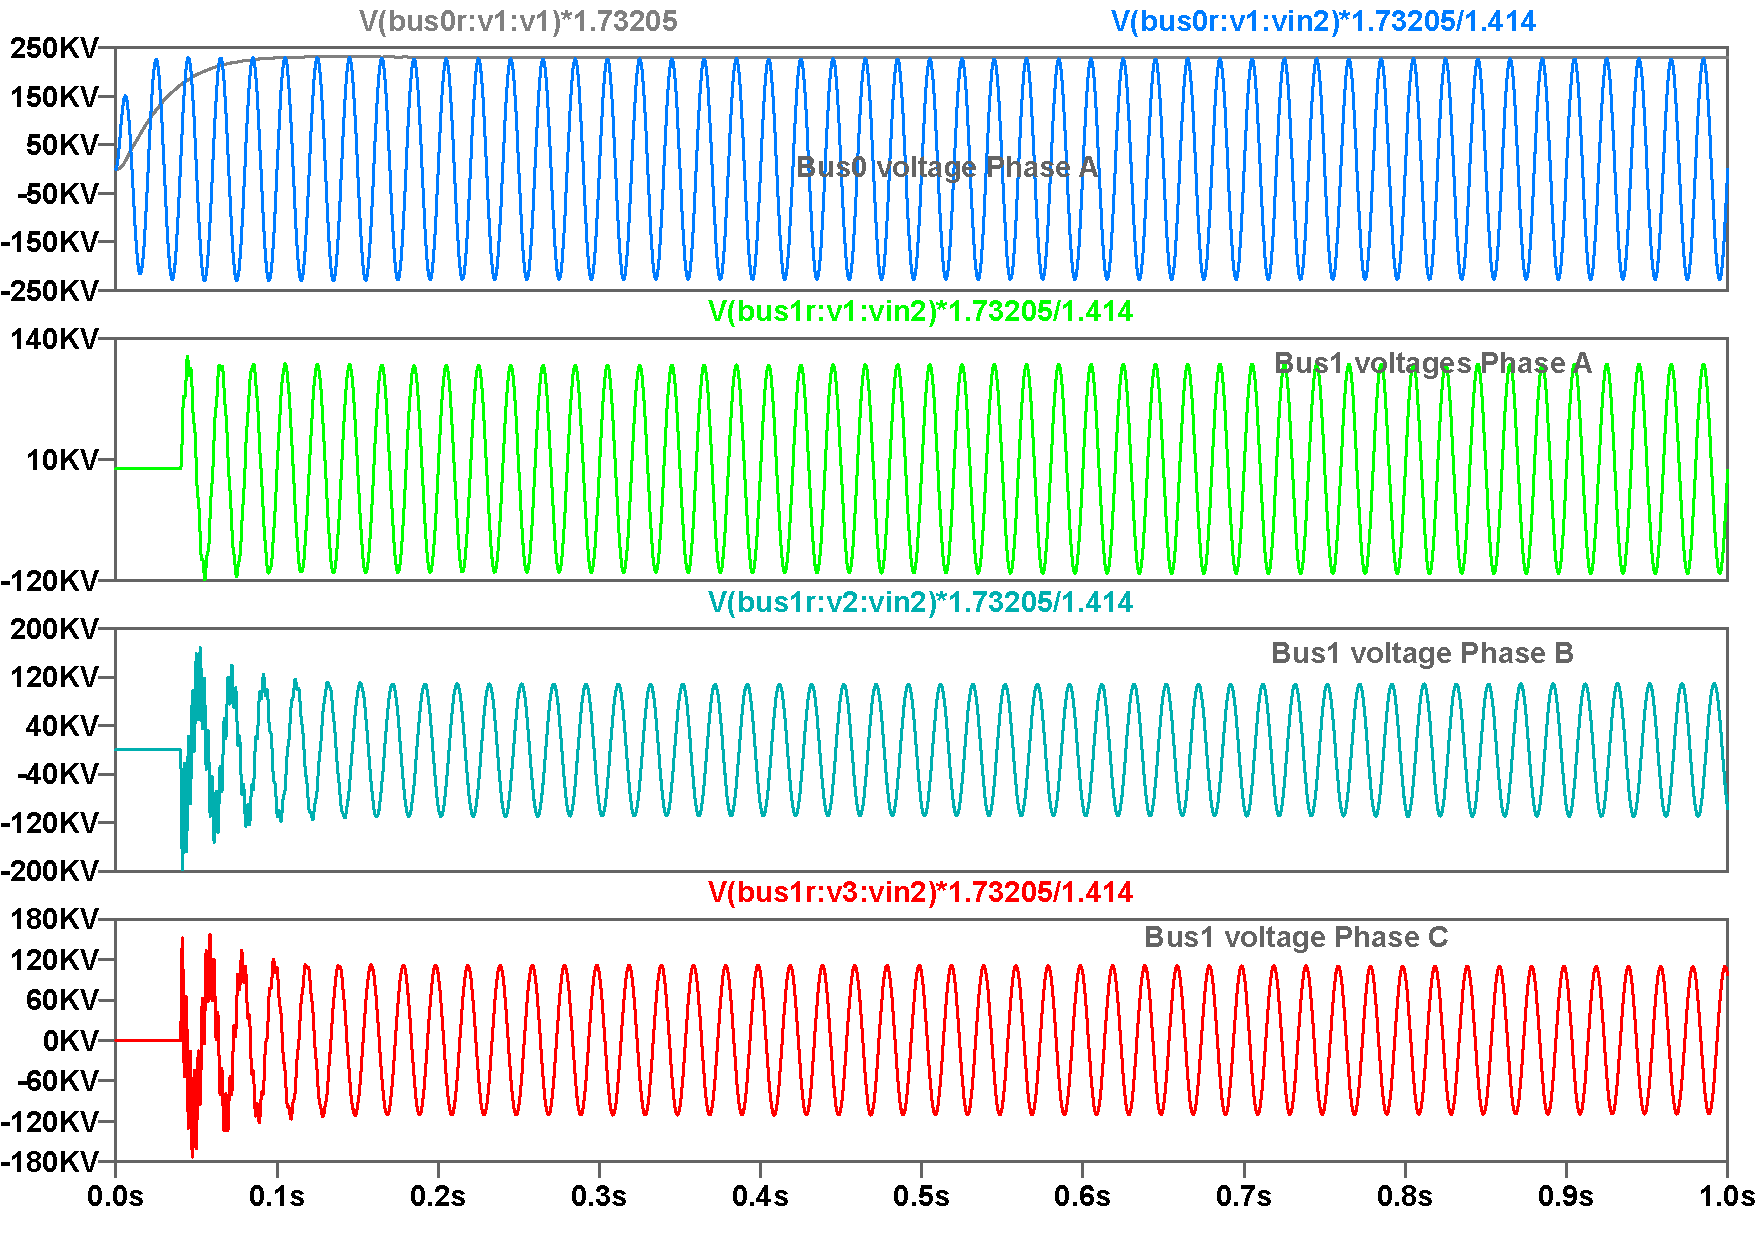
\includegraphics[width=0.90\textwidth]{figures/06_Switching_on_networks/Switching_on_networks_Bus0_Bus1_voltages-case6}
	\caption{Switching on networks voltages - case6}
	\label{fig:figure625}
\end{figure}

\begin{figure}[H]
	\centering
	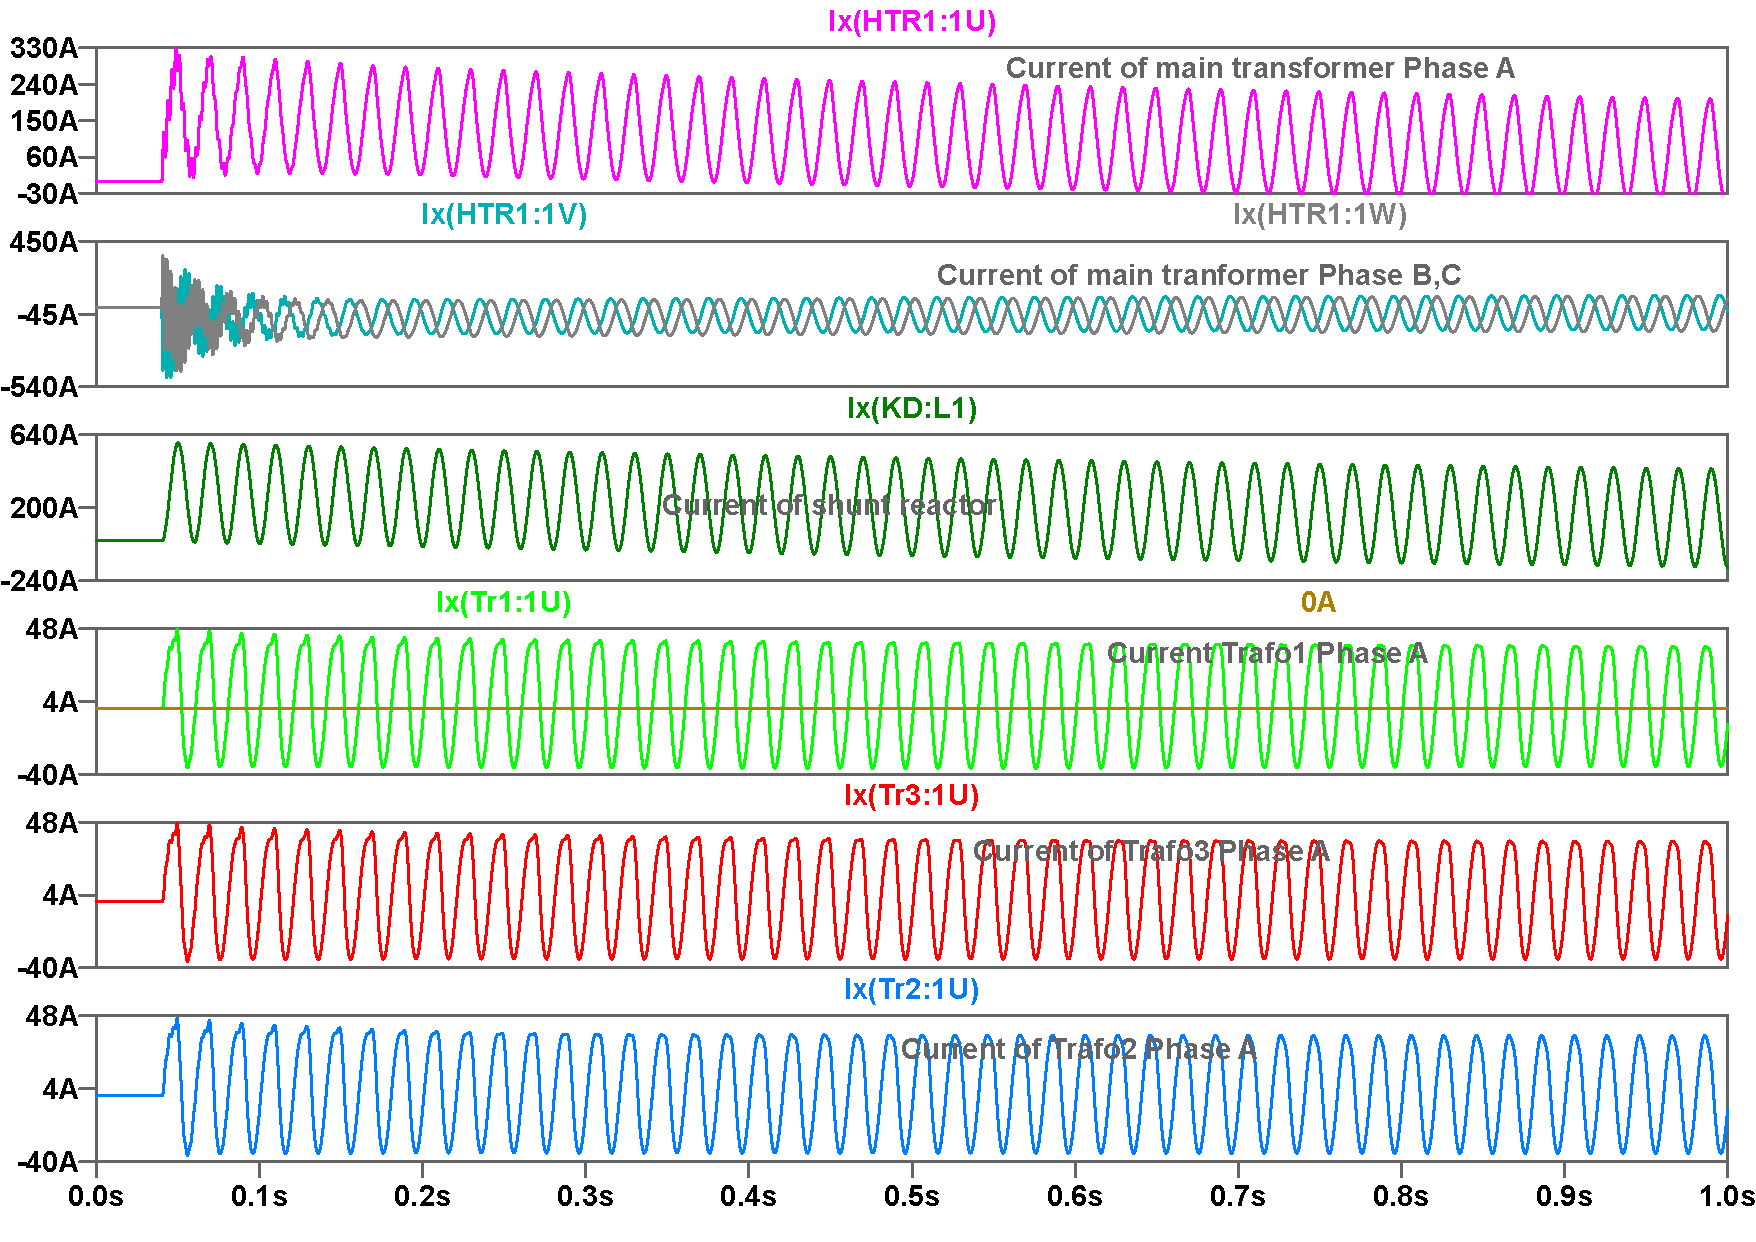
\includegraphics[width=0.90\textwidth]{figures/06_Switching_on_networks/Switching_on_networks_currents-case6}
	\caption{Switching on networks currents - case6}
	\label{fig:figure626}
\end{figure}

\begin{figure}[H]
	\centering
	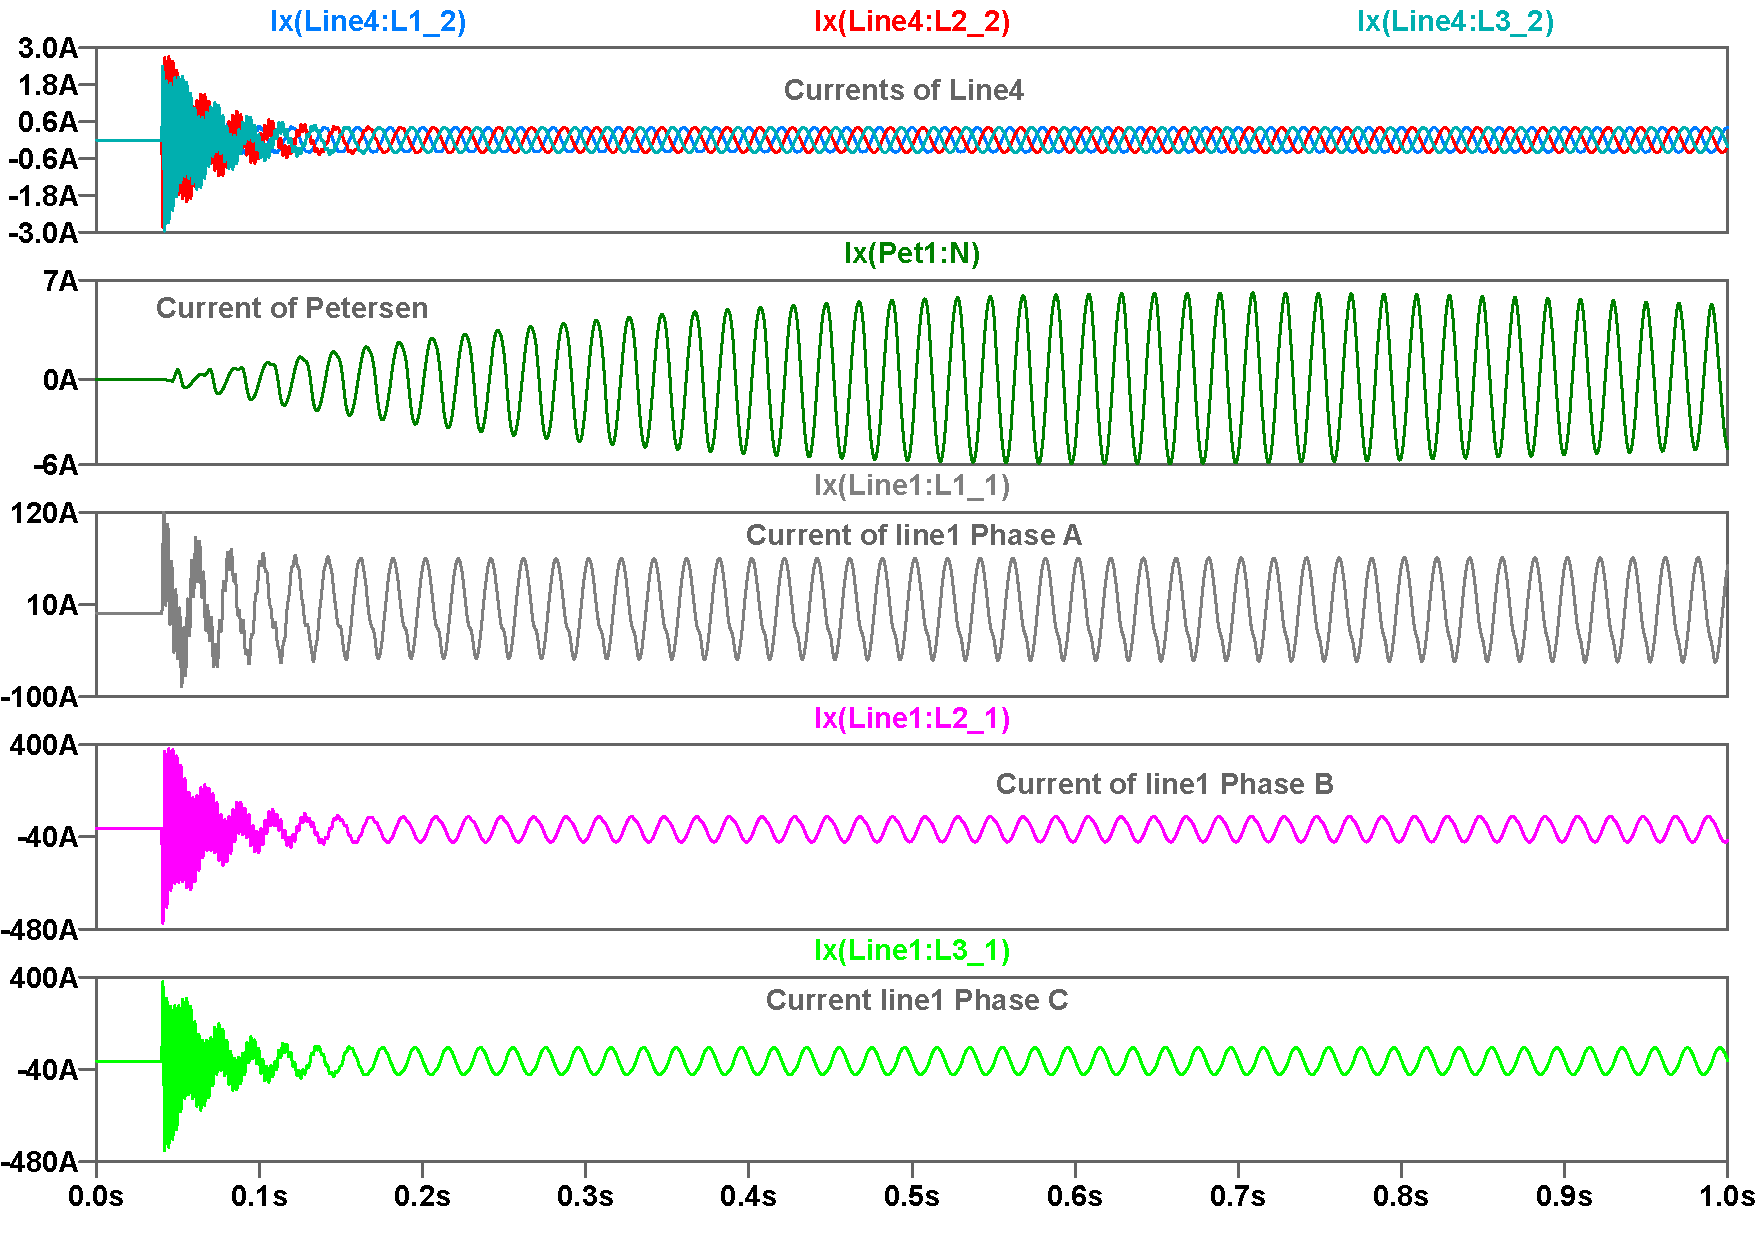
\includegraphics[width=0.90\textwidth]{figures/06_Switching_on_networks/Switching_on_networks_currents_Line1_Line4-case6}
	\caption{Switching on networks currents line1, line4 - case6}
	\label{fig:figure627}
\end{figure}

\begin{figure}[H]
	\centering
	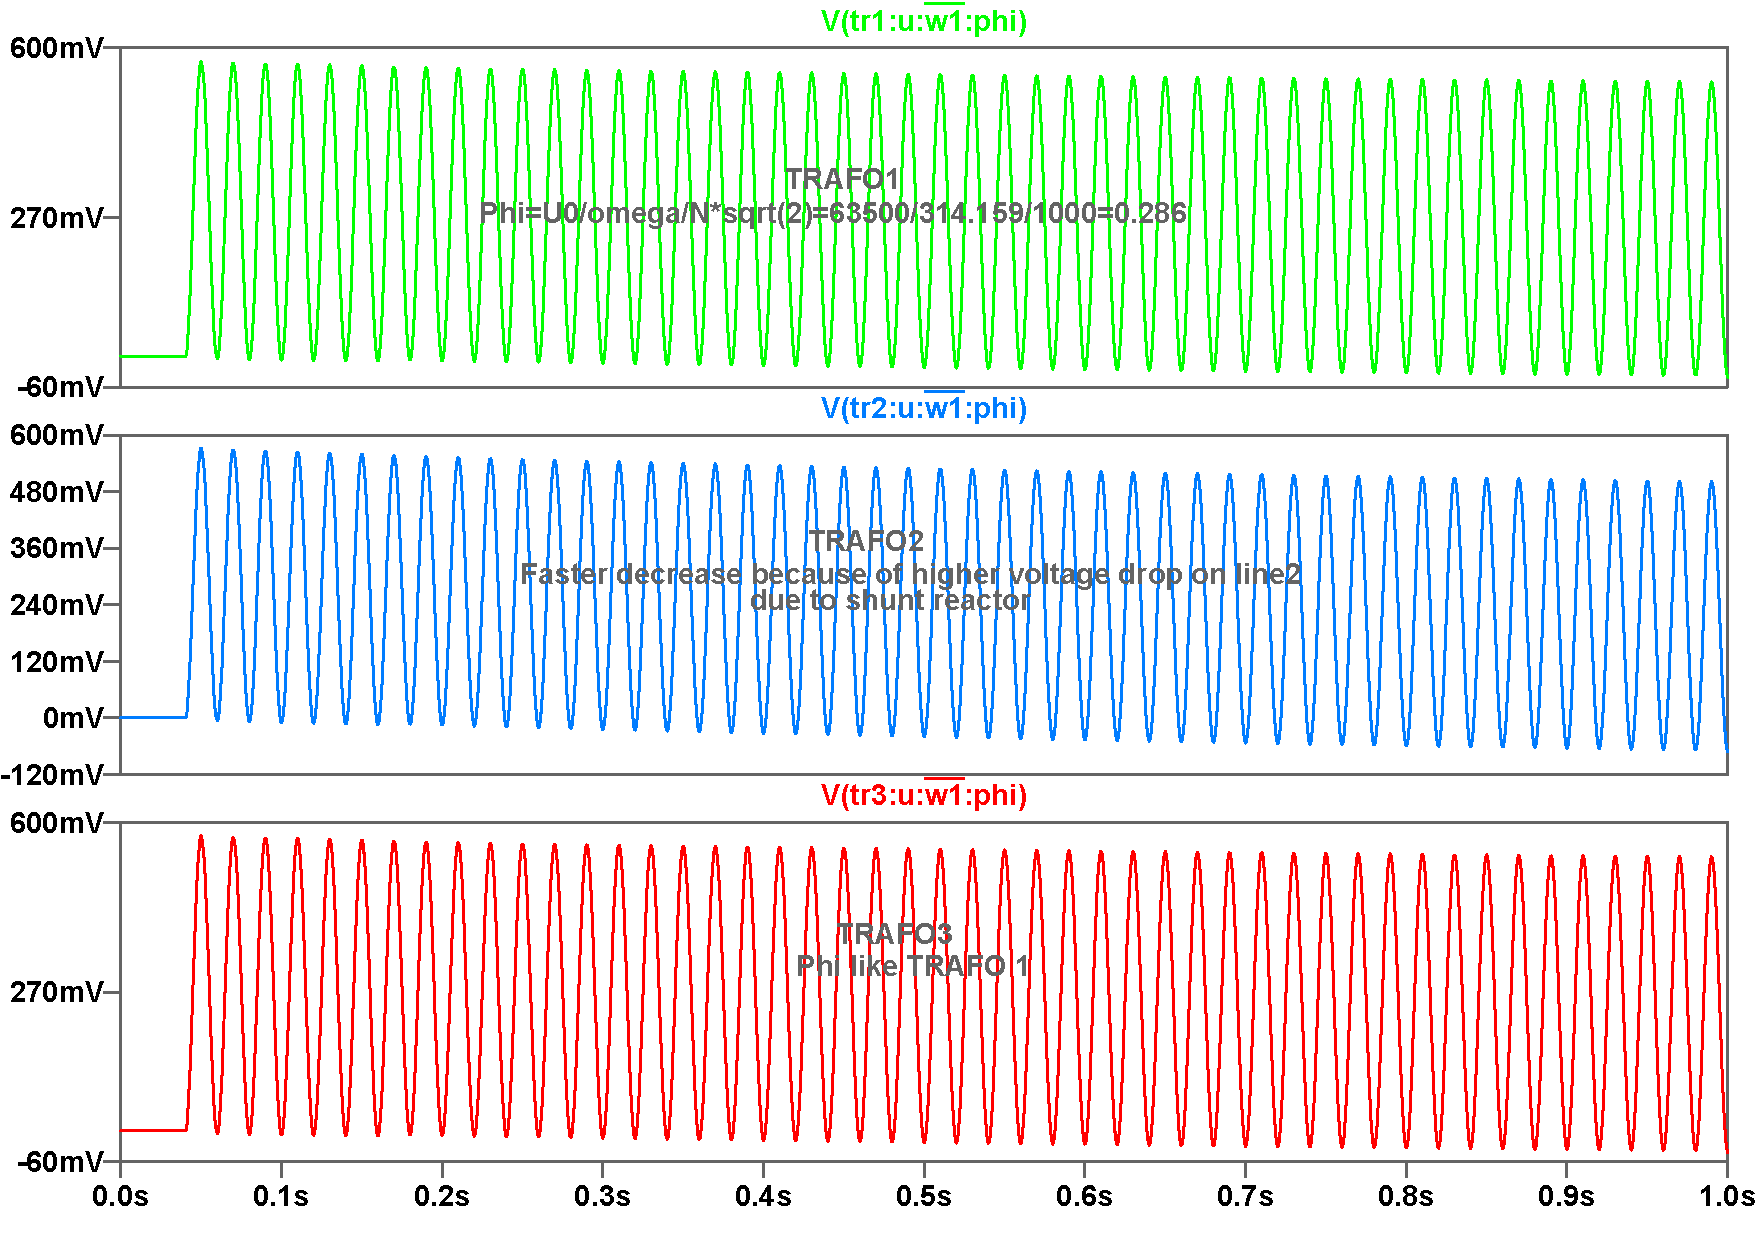
\includegraphics[width=0.90\textwidth]{figures/06_Switching_on_networks/Switching_on_networks_phi-case6}
	\caption{Switching on networks fluxes - case6}
	\label{fig:figure628}
\end{figure}


% Measurement values table for the Power System Simulation book.
% Required packages are already loaded by the central preamble:
% booktabs, tabularx, array, siunitx, xcolor.

\begin{table}[htbp]
  \centering
  \caption{Signal ranges for Case 6. All values are peak values, bus values are multiplied by 1.73/1.414}
  \label{tab:measurement-values-case6}
  \small
  \setlength{\tabcolsep}{3.5pt}
  \renewcommand{\arraystretch}{1.18}
  \begin{tabularx}{\textwidth}{@{}
      >{\raggedright\arraybackslash}p{0.055\textwidth}
      >{\raggedright\arraybackslash}p{0.085\textwidth}
      >{\raggedright\arraybackslash}p{0.095\textwidth}
      >{\raggedright\arraybackslash}p{0.105\textwidth}
      >{\raggedright\arraybackslash}p{0.075\textwidth}
      >{\raggedright\arraybackslash}p{0.075\textwidth}
      Y@{}}
    \toprule
    \textbf{Meas.} &
    \textbf{Grid element} &
    \textbf{Phase} &
    \textbf{Voltage level} &
    \textbf{Min.} &
    \textbf{Max.} &
    \textbf{Notes} \\
    \midrule
    $V$ & Bus0  & Ph A       & \SI{220}{\kilo\volt} & \SI{-229}{\kilo\volt} & \SI{229}{\kilo\volt} & -- \\
    $V$ & Bus1  & Ph A,    & \SI{110}{\kilo\volt} & \SI{-120}{\kilo\volt} & \SI{120}{\kilo\volt} & -- \\
    $V$ & Bus1  & Ph B,C     & \SI{110}{\kilo\volt} & \SI{-170}{\kilo\volt} & \SI{160}{\kilo\volt} & -- \\
    $I$ & HTr1  & Ph A       & \SI{220}{\kilo\volt} & \SI{0}{\ampere} & \SI{330}{\ampere} & -- \\
    $I$ & HTr1  & Ph B, C    & \SI{220}{\kilo\volt} & \SI{-480}{\ampere} & \SI{360}{\ampere} & -- \\
    $I$ & KD1   & Ph A       & \SI{110}{\kilo\volt} & \SI{0}{\ampere} & \SI{590}{\ampere} & Steady state: \SI{300}{\ampere} \\
    $I$ & Tr1   & Ph A       & \SI{110}{\kilo\volt} & \SI{-36}{\ampere} & \SI{54}{\ampere} & under load \\
    $I$ & Tr2   & Ph A       & \SI{110}{\kilo\volt} & \SI{-36}{\ampere} & \SI{50}{\ampere} & under load \\
    $I$ & Tr3   & Ph A      & \SI{110}{\kilo\volt} & \SI{-36}{\ampere} & \SI{47}{\ampere} & under load \\
    $I$ & Line4 & Ph A & \SI{110}{\kilo\volt} & \SI{-3}{\ampere} & \SI{2.5}{\ampere} & Small capacitive inrush current  \\
    $I$ & Line1 & Ph A & \SI{110}{\kilo\volt} & \SI{-90}{\ampere} & \SI{120}{\ampere} & High capacitive inrush current due to cable \\
    $I$ & Line1 & Ph B, C & \SI{110}{\kilo\volt} & \SI{-480}{\ampere} & \SI{380}{\ampere} & High capacitive inrush current due to cable \\
    $I$ & Pet1 & Ph N & \SI{110}{\kilo\volt} & \SI{-6}{\ampere} & \SI{6}{\ampere} & Longtime value very small \\
    $V$ & Pet1 & Ph N & \SI{110}{\kilo\volt} & \SI{-1.5}{\kilo\volt} & \SI{1.5}{\kilo\volt} & Longtime value very small \\
    $\Phi$ & Tr1 & Ph A, B, C   & \SI{110}{\kilo\volt} & \SI{0}{\weber} & \SI{0.575}{\weber} & Nominal flux: 
    \SI{0.288}{\weber} \\
    \bottomrule
  \end{tabularx}
\end{table}

 
 
  

\section{Case 7: Skin-Effect Model}
\label{sec:network-skin-effect}

Set \texttt{skin=1}. To apply the skin effect in a rough way, we make the simplified assumption that up to 40 ms, only the 50 Hz component determines the resistance, and from 40 ms onward, only the higher frequency of 400 Hz determines the resistance. (Normally, the 50 Hz and 400 Hz components contribute equally). This allows us to roughly determine the influence of the higher frequency. We see that the additional damping is present but small. Even smaller when split between 50 Hz and 400 Hz. 
The effect is expected to be more pronounced in smaller networks with higher
natural frequencies, particularly when individual lines are energized.

\begin{figure}[H]
	\centering
	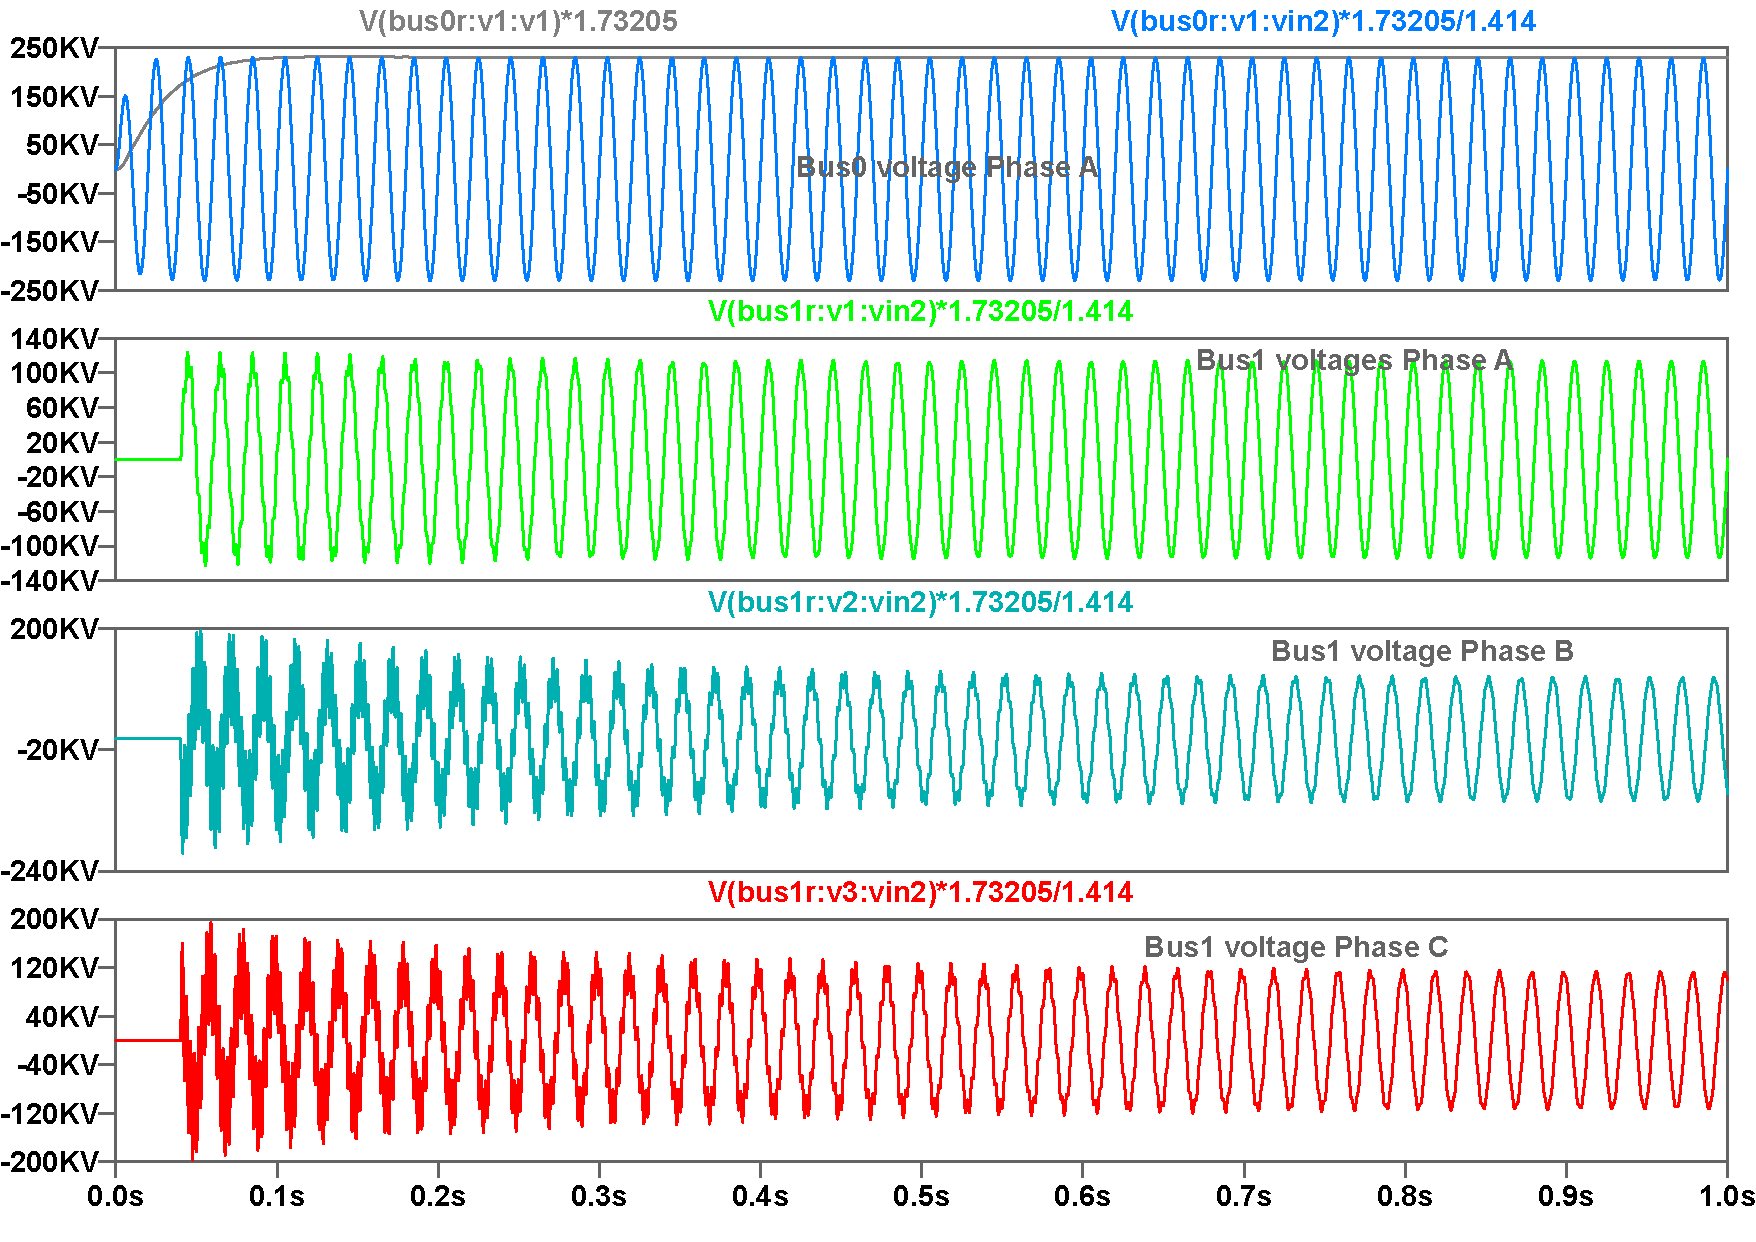
\includegraphics[width=0.90\textwidth]{figures/06_Switching_on_networks/Switching_on_networks_Bus0_Bus1_voltages-case7}
	\caption{Switching on networks voltages - case7}
	\label{fig:figure629}
\end{figure}


\section{Case 8: Energization from a Weak Network}

Set \texttt{weak=40} to increase the source impedance (This setting represents an additional transformer in series, as may occur during restoration after a blackout). The larger source
impedance limits the inrush current, although it may simultaneously increase
voltage sensitivity elsewhere in the network. Due to the higher voltage volatility, it is not advisable to use a shunt reactor in this circuit. It is better to regulate the voltage by tap-changing the transformer. Try it out and observe the steady-state value of the 110kV voltages. 
The 110kV steady state voltage is about 106kV with shunt reactor and 120kV without shunt reactor. There is a voltage drop of about 15kV !!
To see the difference in one plot add the line \texttt{.step param kd list 0 1} to the schematic !!

\begin{figure}[H]
	\centering
	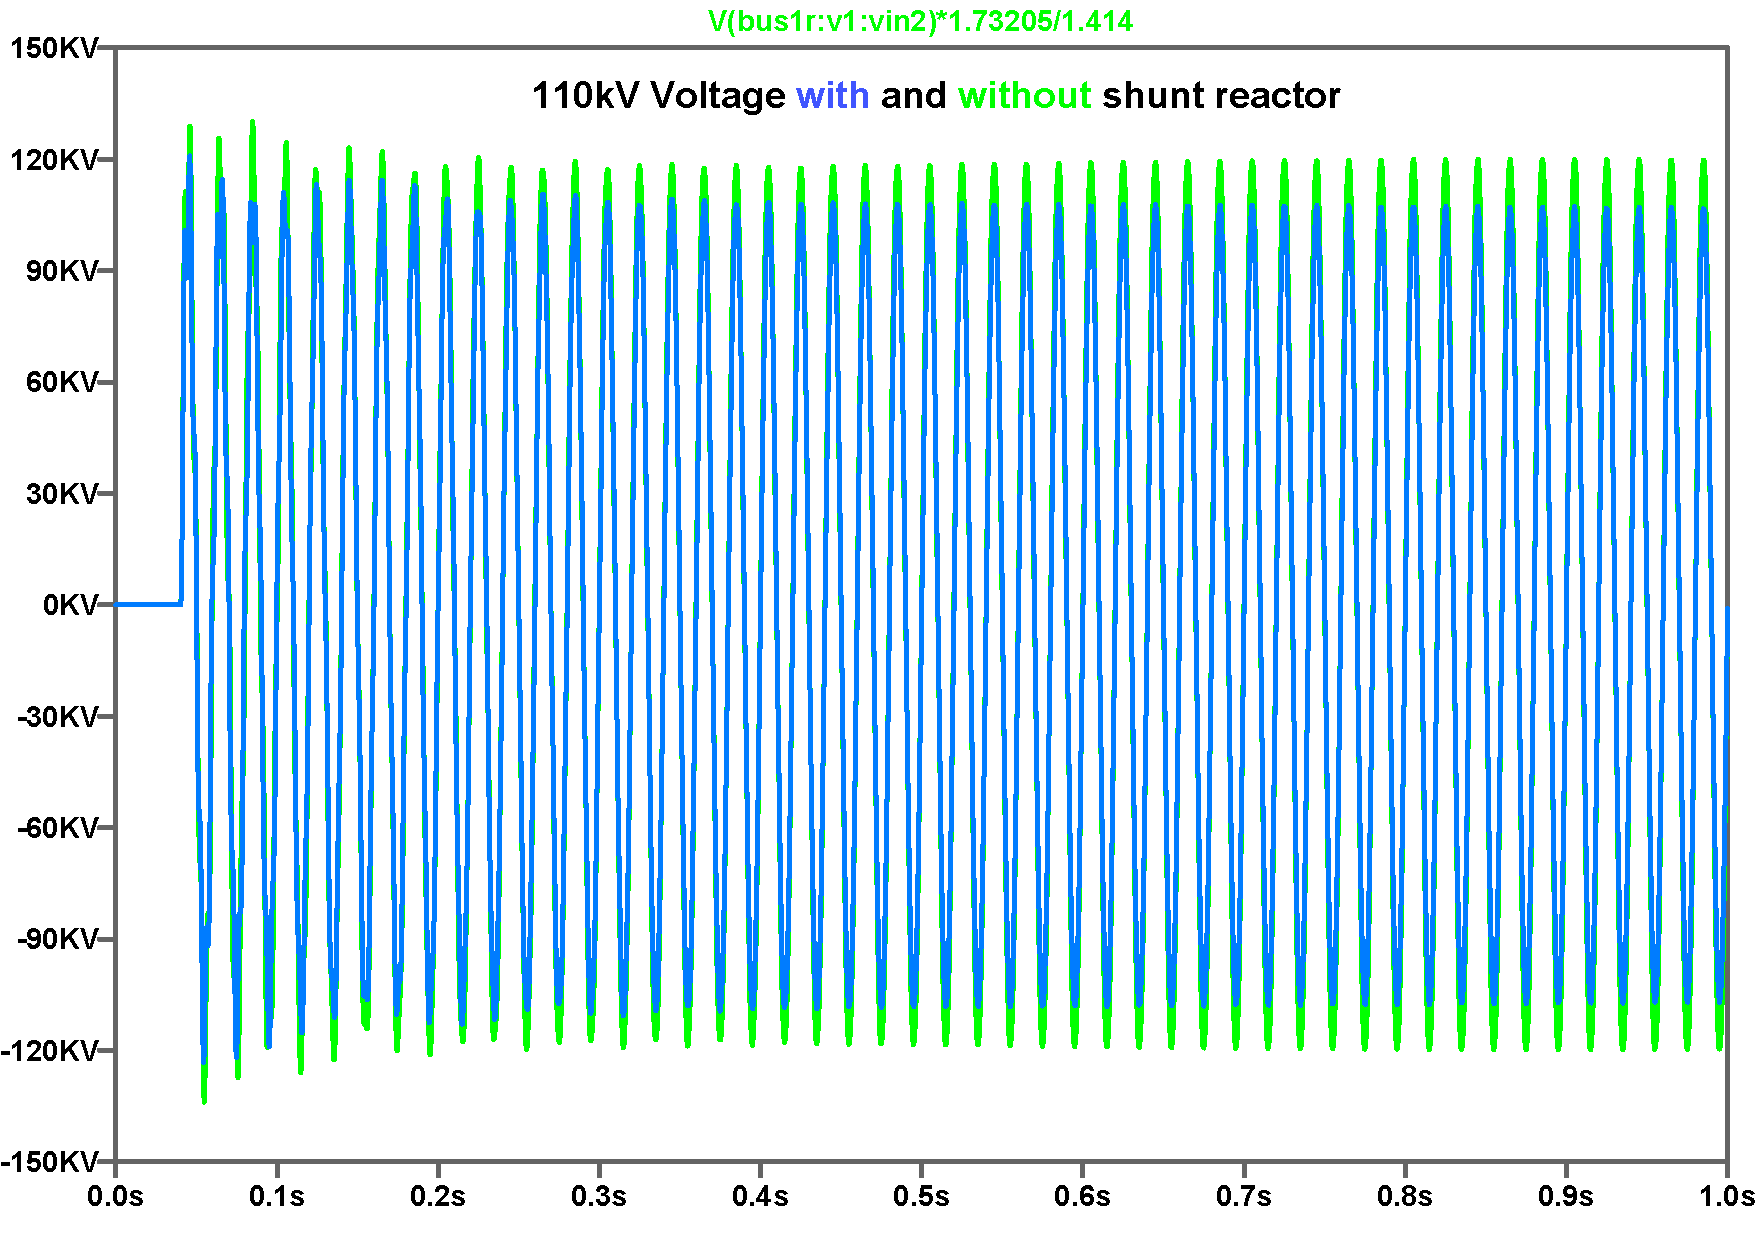
\includegraphics[width=0.90\textwidth]{figures/06_Switching_on_networks/Switching_on_networks_kd_on_off_case8}
	\caption{Switching on networks voltages - case8}
	\label{fig:figure630}
\end{figure}


\section{Case 9: Network Startup by a Voltage Ramp}
\label{sec:network-voltage-ramp}

The simulation file is
\texttt{Switching\_on\_networks\_Voltagetrip.asc}. Set the voltage-source parameter 
\texttt{tpwl} to \SI{400}{\milli\second} and remove the network
switch. Set the parameter ST to 10s to disable it. The source voltage then increases gradually from zero to its nominal
value within 400ms. NOTE: This is not really done in practice but in simulation
to keep the simulation time short.

This procedure produces practically no switching transients: there are no
significant over-voltages, high-frequency charging-current oscillations, or
transformer magnetizing inrush currents. It is therefore the preferred method
for energizing the complete network in this study. Loads should be connected
only after the voltage has reached its nominal level.
The currents of this network are only the charging currents of the lines
and the current of the shunt reactor. 
The magnetizing currents of the transformers 2 and 3 are below 1A.
The current of Transformer1 is a little bit higher due to the current needed by the Petersen.
The currents in all three phases of line 1 have the same amplitude.
The Petersen current is 7A, the Petersen voltage is approximately 1.7kV (measured at time=100s) and the Line4 current is about 400mA.
The flux of transformer 1,2 and 3 have equal amplitudes and about the nominal flux (a little bit higher since the operating voltage is not 110kV).
The 110kV voltage is at about 110kV in phase A 113.7kV in Phase B and 112.3kV in Phase C (slightly different because of the neutral point displacement voltage) which is the steady-state value.
The FFT shows only the nominal frequency of 50Hz for the whole circuit !! 

\begin{figure}[H]
	\centering
	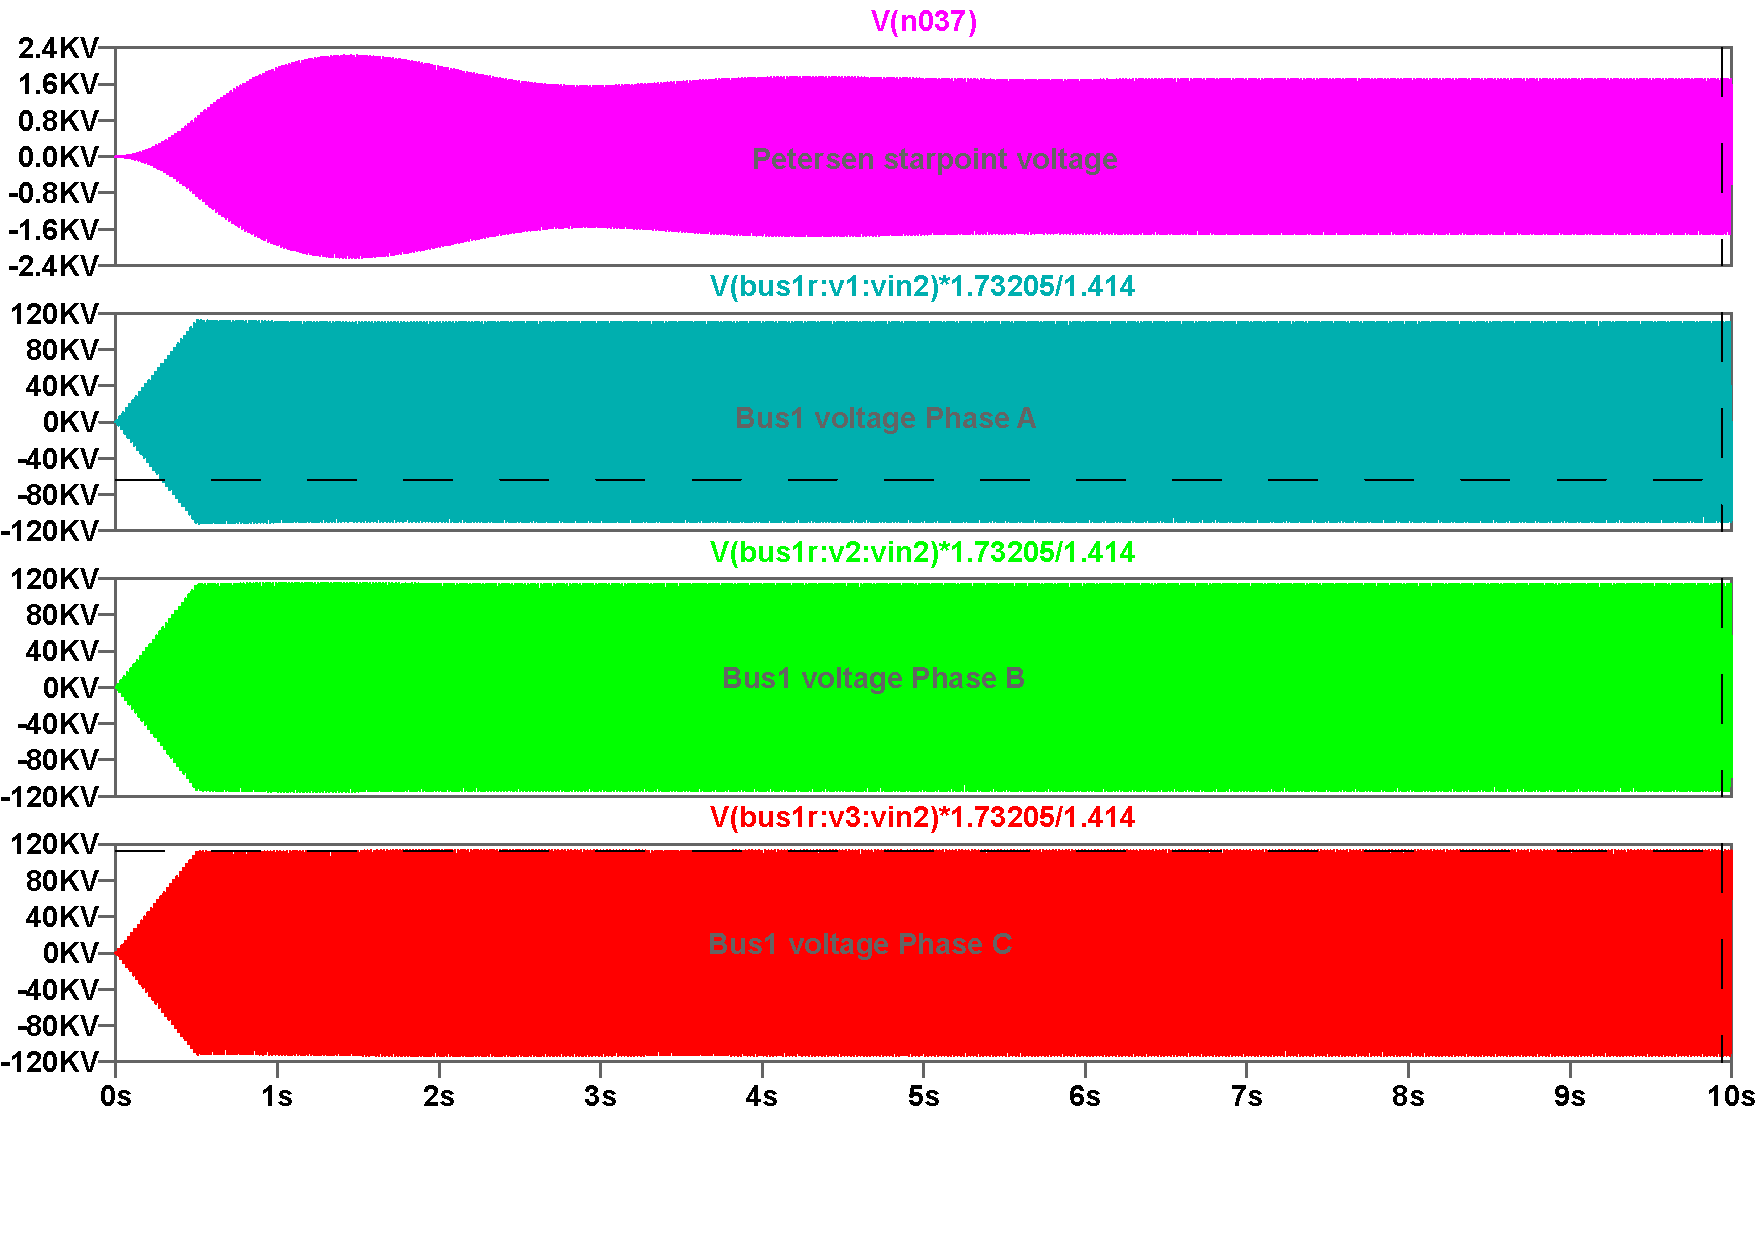
\includegraphics[width=0.90\textwidth]{figures/06_Switching_on_networks/Switching_on_networks_Bus0_Bus1_voltages-case9}
	\caption{Switching on networks voltage-trip, voltages - case9}
	\label{fig:figure625}
\end{figure}

\begin{figure}[H]
	\centering
	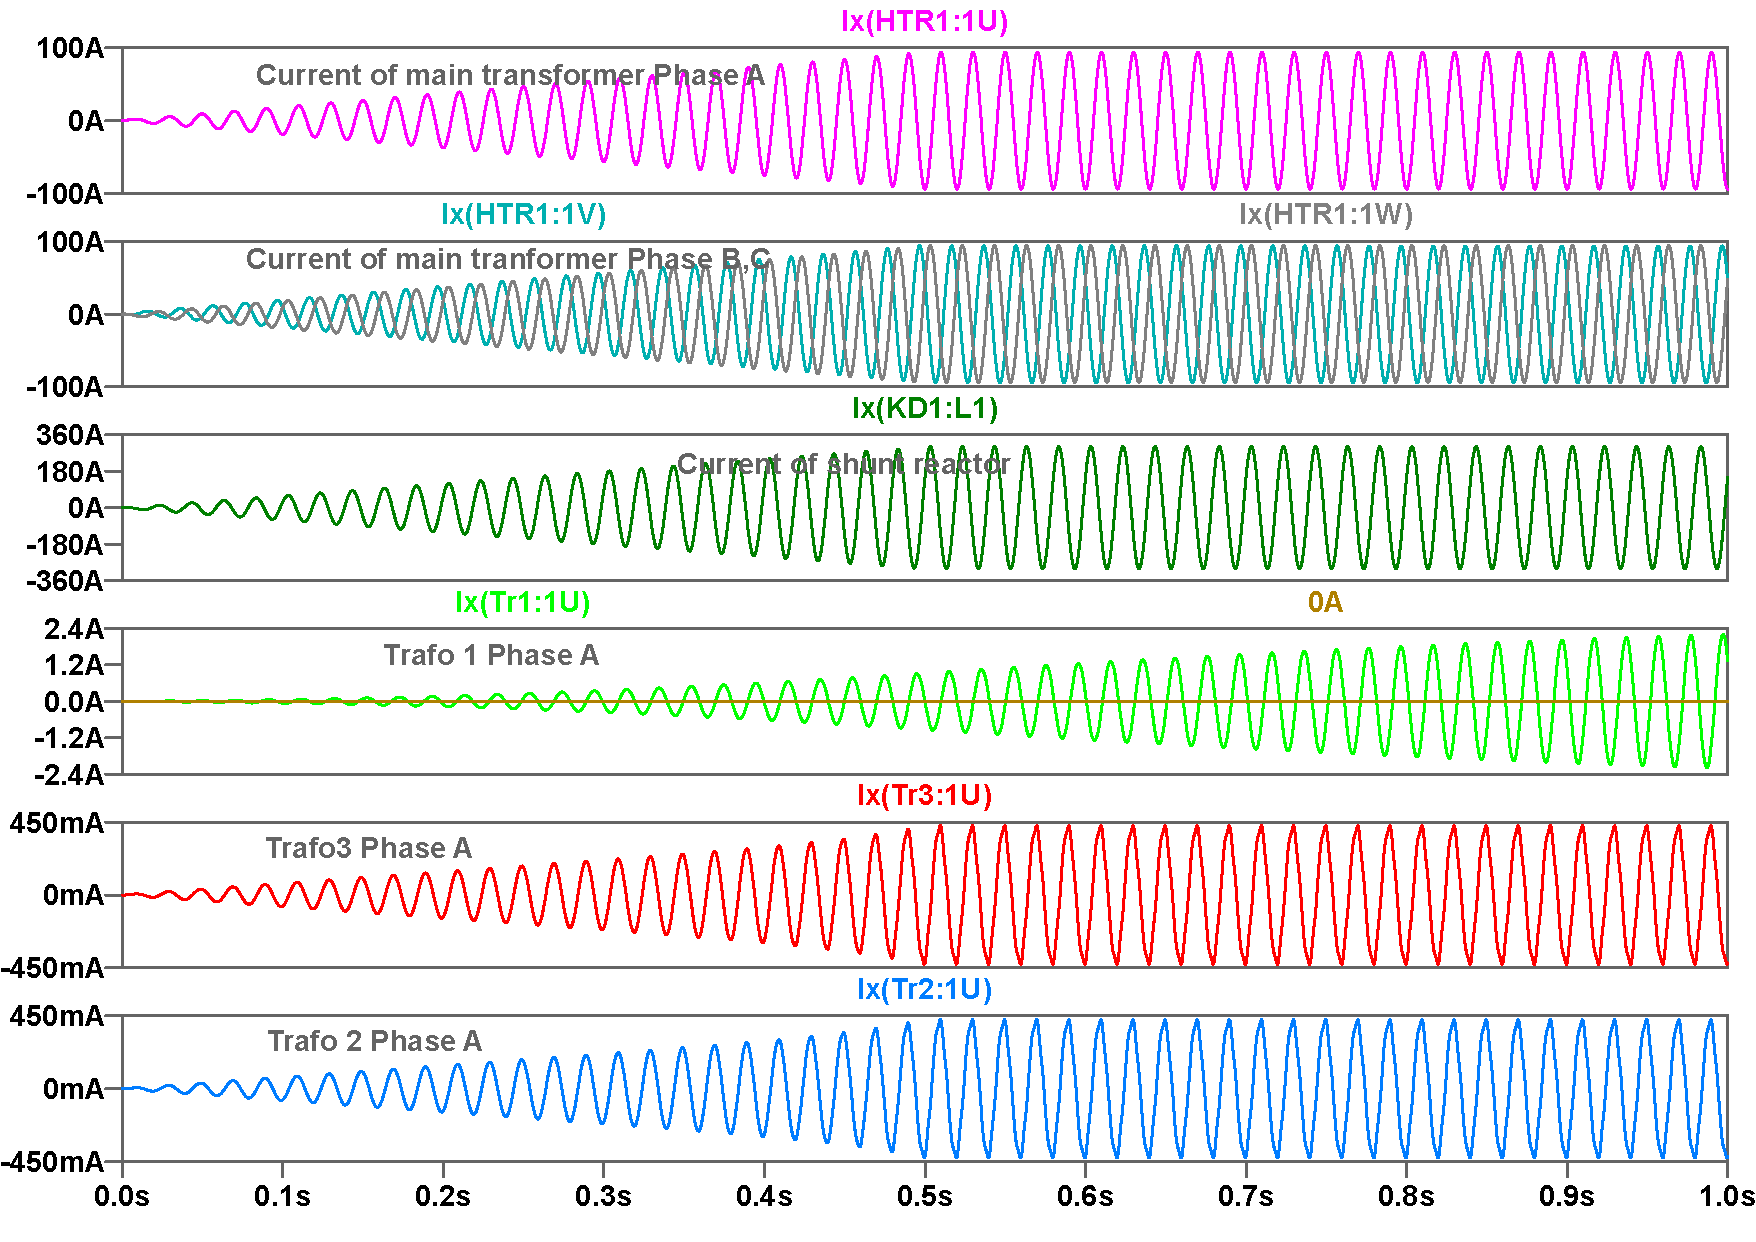
\includegraphics[width=0.90\textwidth]{figures/06_Switching_on_networks/Switching_on_networks_currents-case9}
	\caption{Switching on networks voltage-trip, currents - case9}
	\label{fig:figure626}
\end{figure}

\begin{figure}[H]
	\centering
	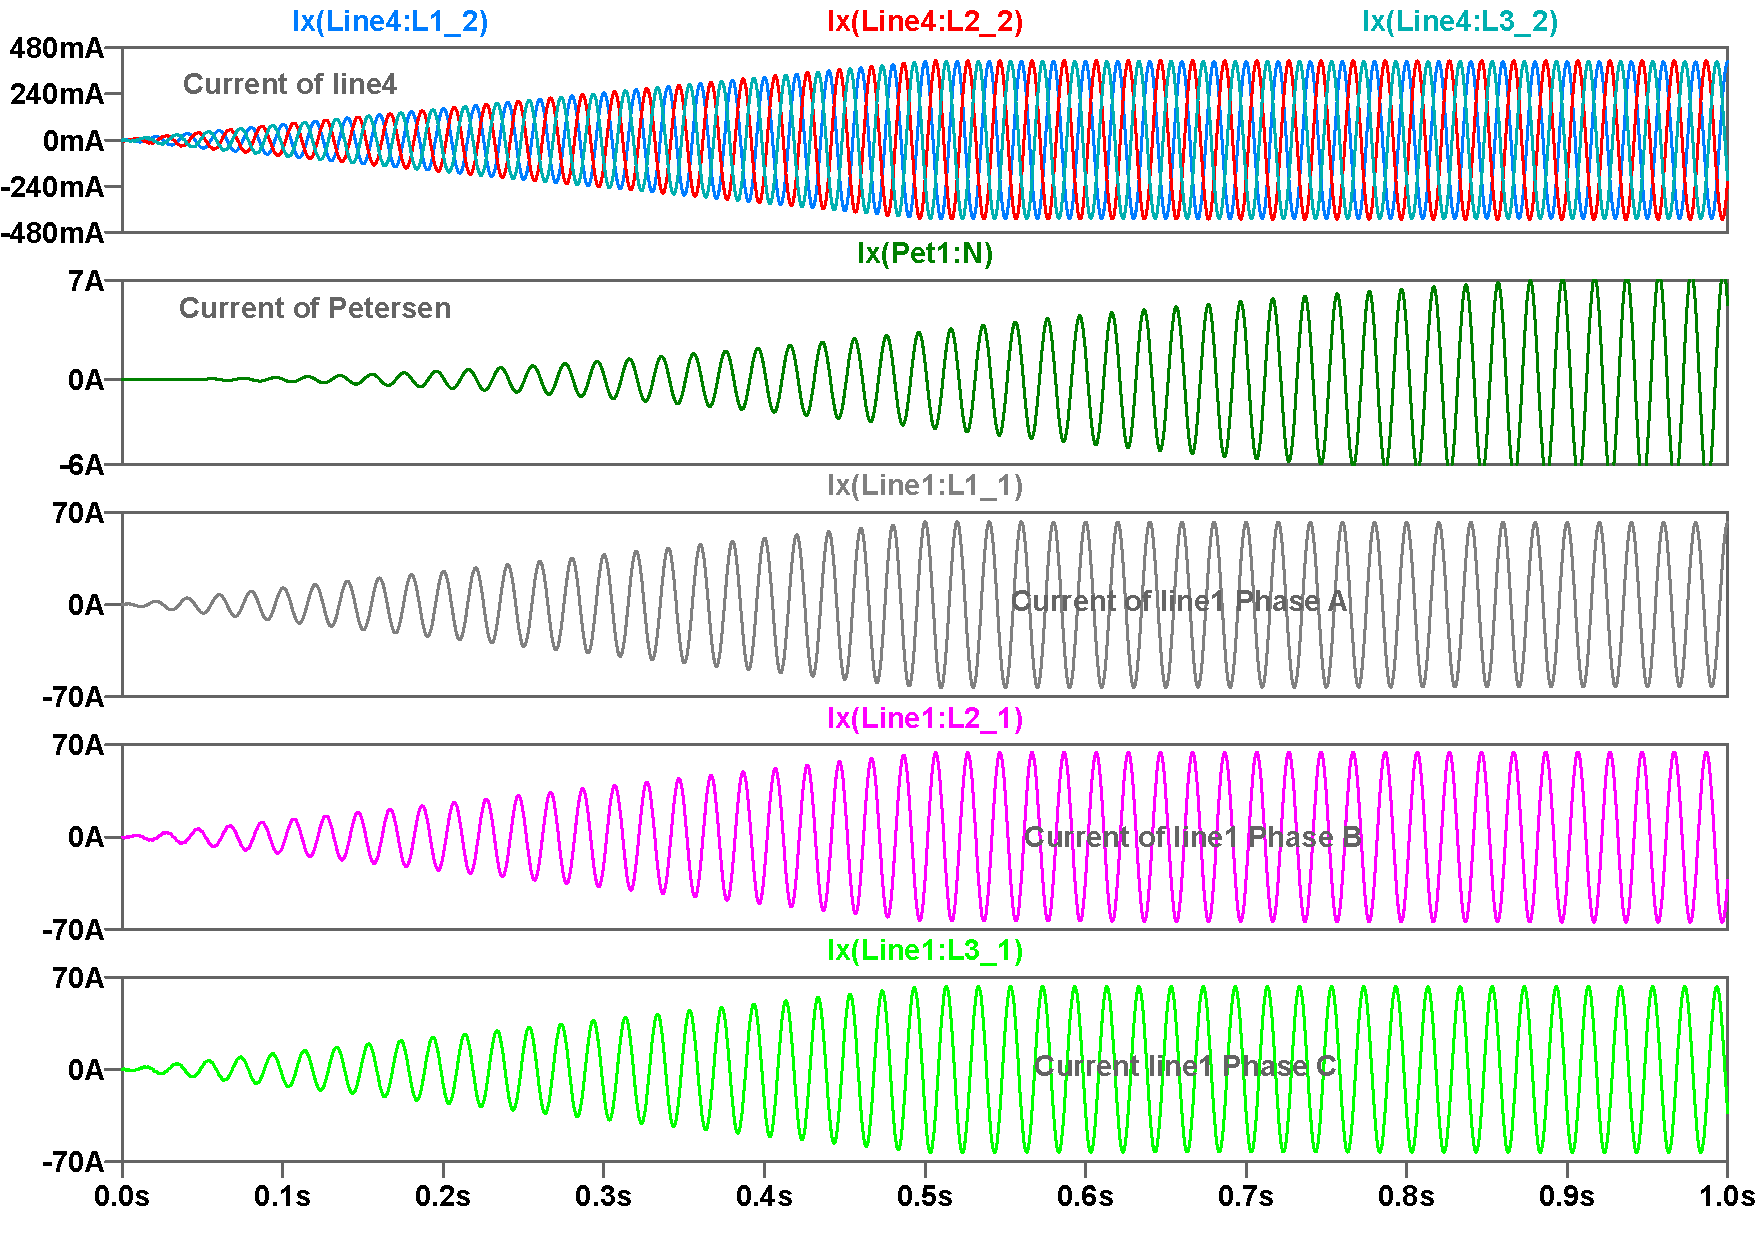
\includegraphics[width=0.90\textwidth]{figures/06_Switching_on_networks/Switching_on_networks_currents_Line1_Line4-case9}
	\caption{Switching on networks voltage-trip, currents line1, line4 - case9}
	\label{fig:figure627}
\end{figure}

\begin{figure}[H]
	\centering
	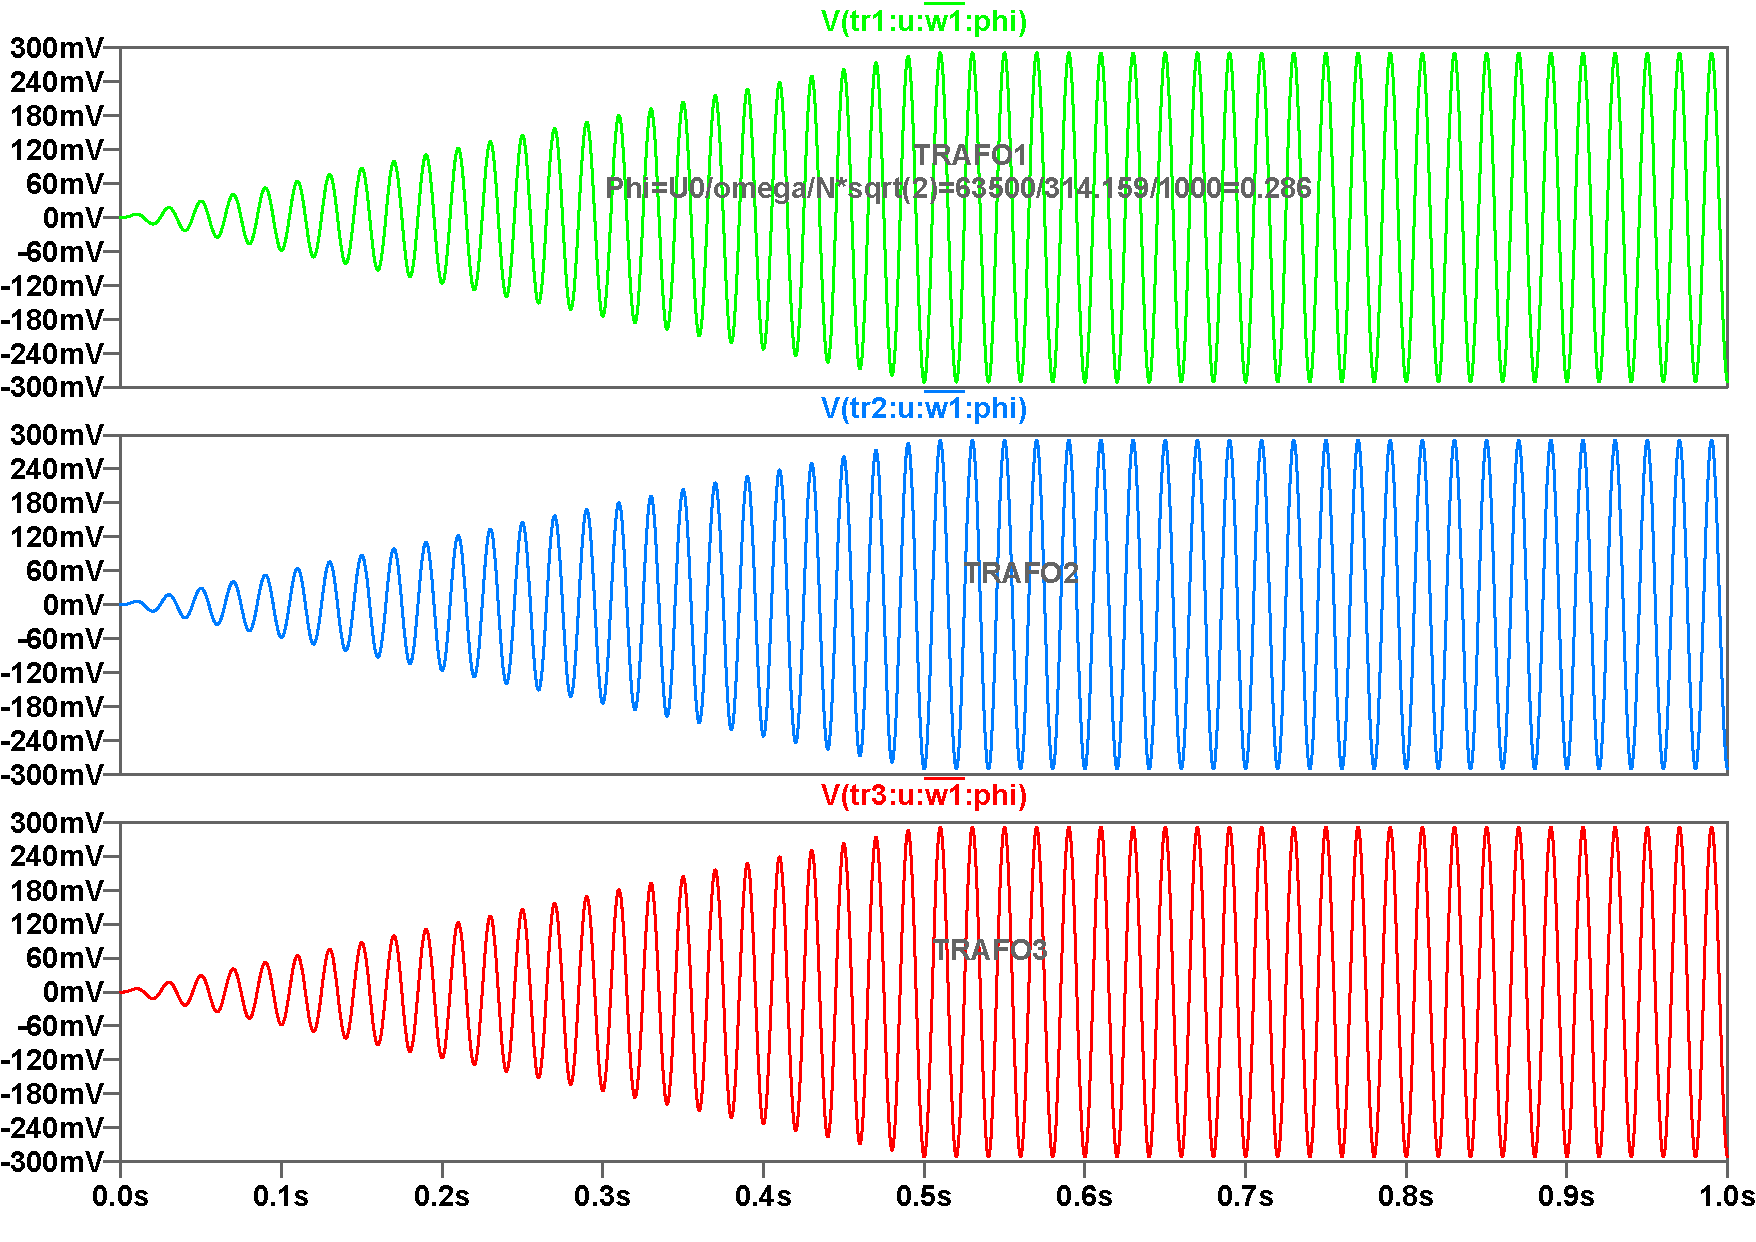
\includegraphics[width=0.90\textwidth]{figures/06_Switching_on_networks/Switching_on_networks_phi-case9}
	\caption{Switching on networks voltage-trip, fluxes - case9}
	\label{fig:figure628}
\end{figure}

\begin{figure}[H]
	\centering
	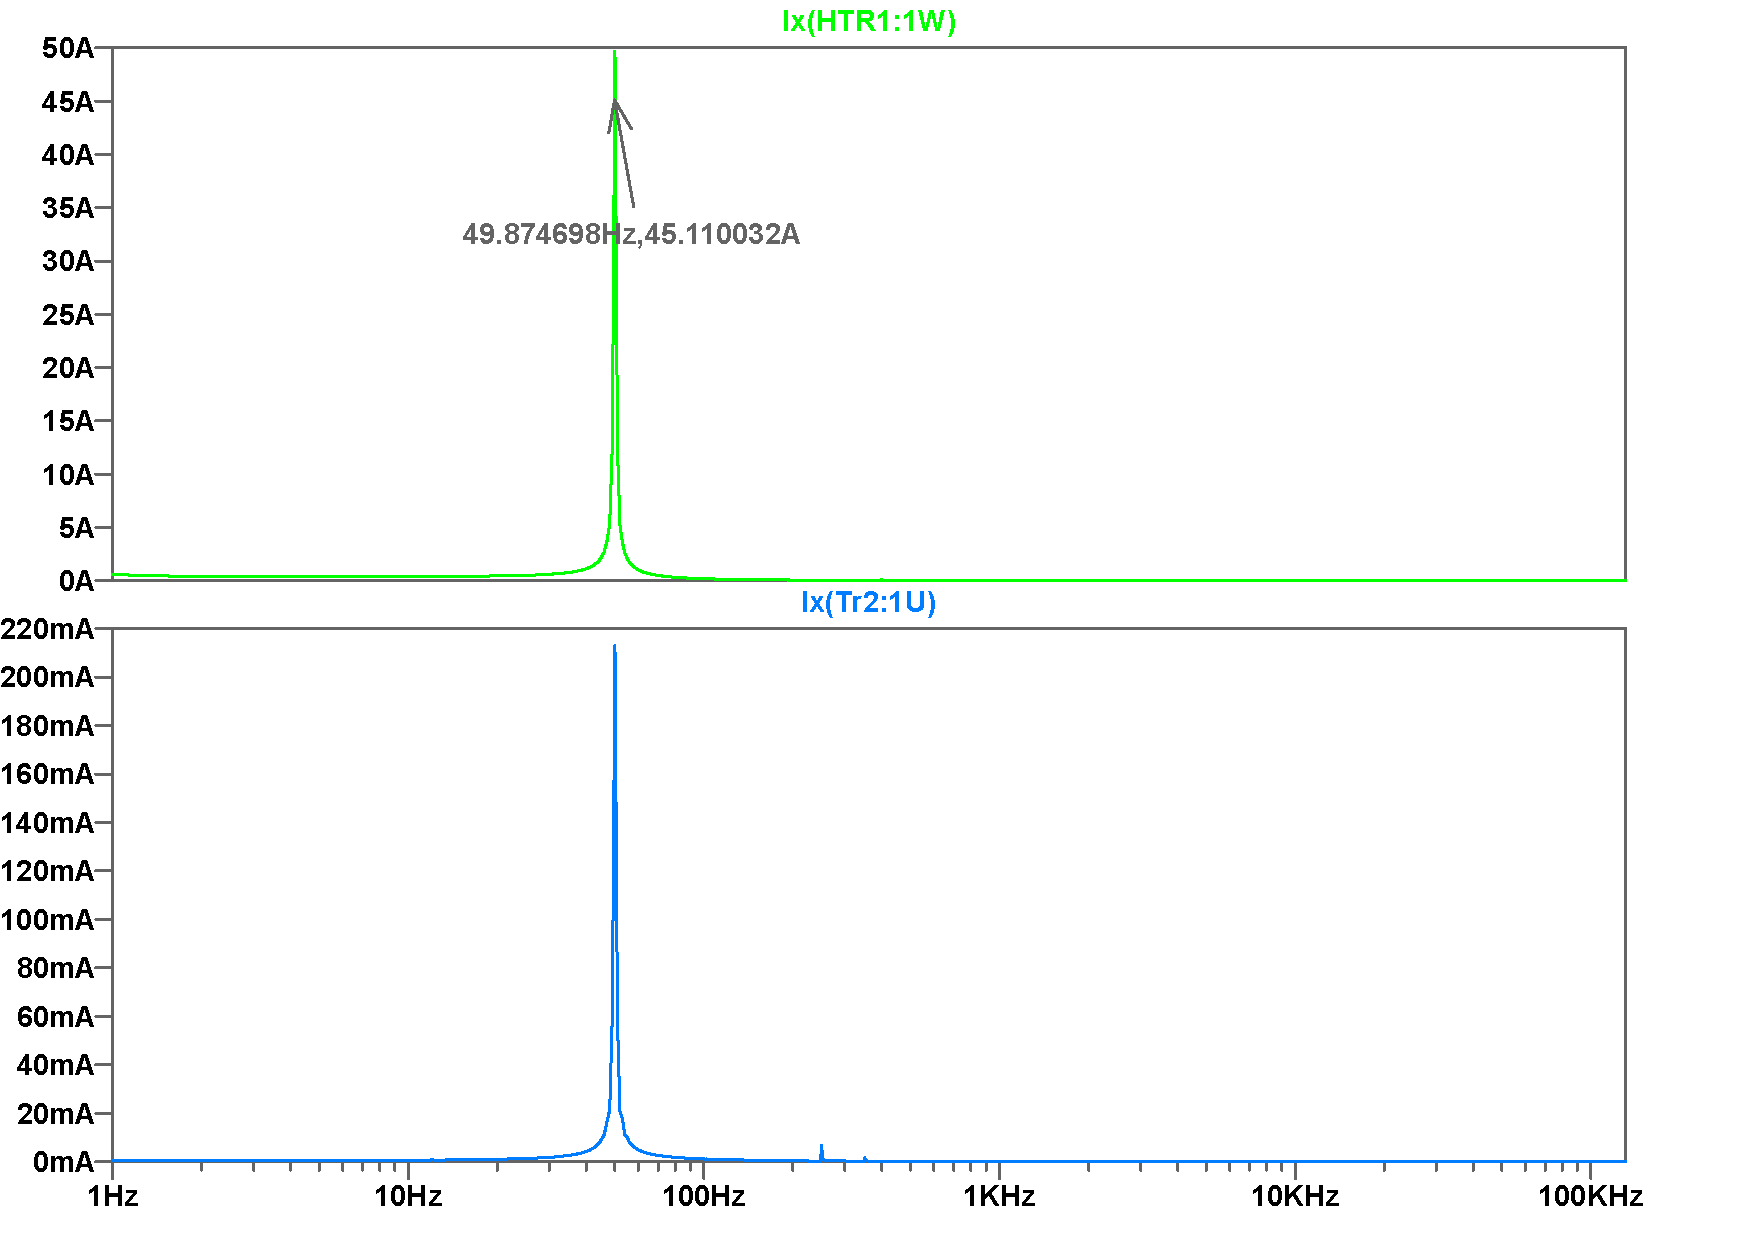
\includegraphics[width=0.90\textwidth]{figures/06_Switching_on_networks/Switching_on_networks_FFT_Transformer-case9}
	\caption{Switching on networks voltage-trip, FFT - case9}
	\label{fig:figure629}
\end{figure}


% Measurement values table for the Power System Simulation book.
% Required packages are already loaded by the central preamble:
% booktabs, tabularx, array, siunitx, xcolor.

\begin{table}[htbp]
  \centering
  \caption{Signal ranges for Case 9. All values are peak values, bus values are multiplied by 1.73/1.414}
  \label{tab:measurement-values-case9}
  \small
  \setlength{\tabcolsep}{3.5pt}
  \renewcommand{\arraystretch}{1.18}
  \begin{tabularx}{\textwidth}{@{}
      >{\raggedright\arraybackslash}p{0.055\textwidth}
      >{\raggedright\arraybackslash}p{0.085\textwidth}
      >{\raggedright\arraybackslash}p{0.095\textwidth}
      >{\raggedright\arraybackslash}p{0.105\textwidth}
      >{\raggedright\arraybackslash}p{0.075\textwidth}
      >{\raggedright\arraybackslash}p{0.075\textwidth}
      Y@{}}
    \toprule
    \textbf{Meas.} &
    \textbf{Grid element} &
    \textbf{Phase} &
    \textbf{Voltage level} &
    \textbf{Min.} &
    \textbf{Max.} &
    \textbf{Notes} \\
    \midrule
    $V$ & Bus0  & Ph A       & \SI{220}{\kilo\volt} & \SI{-229}{\kilo\volt} & \SI{229}{\kilo\volt} & Steady state RMS \\
    $V$ & Bus1  & Ph A       & \SI{110}{\kilo\volt} & \SI{-110}{\kilo\volt} & \SI{110}{\kilo\volt} & Steady state RMS \\
    $V$ & Bus1  & Ph B, C    & \SI{110}{\kilo\volt} & \SI{-113}{\kilo\volt} & \SI{113}{\kilo\volt} & Steady state RMS \\
    $I$ & HTr1  & Ph A       & \SI{220}{\kilo\volt} & \SI{-94}{\ampere} & \SI{94}{\ampere} & Steady state peak \\
    $I$ & HTr1  & Ph B, C    & \SI{220}{\kilo\volt} & \SI{-94}{\ampere} & \SI{94}{\ampere} & Steady state peak \\
    $I$ & KD1   & Ph A       & \SI{110}{\kilo\volt} & \SI{-300}{\ampere} & \SI{300}{\ampere} & Steady state peak \\
    $I$ & Tr1   & Ph A       & \SI{110}{\kilo\volt} & \SI{-2}{\ampere} & \SI{2}{\ampere} & Due to Petersen higher than Tr2,3 \\
    $I$ & Tr2   & Ph A       & \SI{110}{\kilo\volt} & \SI{-450}{\milli\ampere} & \SI{450}{\milli\ampere} & Steady state zero load peak current \\
    $I$ & Tr3   & Ph A      & \SI{110}{\kilo\volt} & \SI{-450}{\milli\ampere} & \SI{450}{\milli\ampere} & Steady state zero load peak current \\
    $I$ & Line4 & Ph A & \SI{110}{\kilo\volt} & \SI{-410}{\milli\ampere} & \SI{410}{\milli\ampere} & Steady state peak   \\
    $I$ & Line1 & Ph A, B, C & \SI{110}{\kilo\volt} & \SI{-62}{\ampere} & \SI{62}{\ampere} & Steady state peak  \\
    $I$ & Pet1 & Ph N & \SI{110}{\kilo\volt} & \SI{-7}{\ampere} & \SI{7}{\ampere} & Steady state peak \\
    $V$ & Pet1 & Ph N & \SI{110}{\kilo\volt} & \SI{-1.7}{\kilo\volt} & \SI{1.7}{\kilo\volt} & Steady state peak \\
    $\Phi$ & Tr1 & Ph A, B, C   & \SI{110}{\kilo\volt} & \SI{0.291}{\weber} & \SI{0.291}{\weber} & Nominal flux: \SI{0.288}{\weber} peak \\
    FFT & HTr1  & Ph C       & \SI{220}{\kilo\volt} & \SI{50}{\hertz} & \SI{50}{\hertz} & only \SI{50}{\hertz} nominal frequ.  \\
    FFT & Tr2   & Ph A       & \SI{110}{\kilo\volt} & \SI{50}{\hertz} & \SI{50}{\hertz} & \SI{50}{\hertz} nominal frequ. \\     
    \bottomrule
  \end{tabularx}
\end{table}





\begin{important}{Preferred energization method}{imp:network-voltage-ramp}
A controlled voltage ramp avoids the abrupt change in applied voltage that
excites cable resonances and transformer flux offsets. The ramp time must be
long compared with the dominant electrical oscillation periods, and load
connection must be delayed until the voltage is established.
\end{important}

\begin{chaptersummary}
Energizing an entire cable-dominated network excites both transformer inrush
and cable-charging transients. The switching instant determines which phases
are dominated by magnetizing current and which by capacitive current. Cable
capacitance, referred transformer inductance, tap position, load, and network
strength determine the natural frequencies and transient amplitudes. Residual
flux can raise transformer currents above rated peak current, while connected
loads add effective damping. In this study, a gradual source-voltage ramp is
the most effective energization method because it suppresses both cable
resonances and transformer inrush.
\end{chaptersummary}
